% Created 2018-04-19 Thu 03:11
% Intended LaTeX compiler: pdflatex
\documentclass[12pt,glossary]{dalthesis}
\usepackage{listings}
\usepackage[a-1b]{pdfx}
%\usepackage[acronym]{glossaries}
\usepackage{algorithmic}
\usepackage[chapter]{algorithm}
\renewcommand{\listalgorithmname}{ }
\usepackage{color}
\usepackage{needspace}
\usepackage{gnuplot-lua-tikz}
\usepackage{multicol,calc,listings}
\lstset{
  basicstyle=\ttfamily,
  keepspaces=true,
  columns=fullflexible,
  escapeinside={(*}{*)}
}
\usepackage{booktabs,url}
%  For formal tables
{\ttfamily \hyphenchar\the\font=`\-} 
\usepackage{makeidx}
\makeindex

\setcounter{secnumdepth}{5}
% Render all text in math sections monospaced
%\everymath{\mathtt{\xdef\tmp{\fam\the\fam\relax}\aftergroup\tmp}}
%\everydisplay{\mathtt{\xdef\tmp{\fam\the\fam\relax}\aftergroup\tmp}}
%\setbox0\hbox{$ $} 

\newcommand\addr[1] {\widehat{#1}}
\newcommand\deref[1] {\breve{#1}}
\newcommand\corn[1] {\ulcorner {#1} \urcorner}
\newcommand\word[1] {$\mathbb{N}^{\,#1}$}

\usepackage[scaled=0.85]{beramono}
\usepackage{quotchap}
\lstset{basicstyle=\footnotesize\ttfamily}
%\makenoidxglossaries
\loadglsentries{glossary}

\usepackage[all]{nowidow}
\usepackage{imakeidx}
\makeindex[title={}]

\widowpenalty10000
\clubpenalty10000

%\fancyhead[L]{}
%\fancyhead[C]{}
%\fancyhead[R]{}
%\fancyfoot[L]{}
%\fancyfoot[R]{}
%%%%%%%%%%%%%%%%%%%%%%%%%%%%%%%%
\usepackage[lmargin=3.81cm,tmargin=2.54cm,bmargin=2.54cm,rmargin=2.54cm]{geometry}

\usepackage{authorindex}
\let\cite=\aicite



\usepackage[utf8]{inputenc}
\usepackage[T1]{fontenc}
\usepackage{graphicx}
\usepackage{grffile}
\usepackage{longtable}
\usepackage{wrapfig}
\usepackage{rotating}
\usepackage[normalem]{ulem}
\usepackage{amsmath}
\usepackage{textcomp}
\usepackage{amssymb}
\usepackage{capt-of}
\usepackage{hyperref}
\date{\today}
\title{}
\hypersetup{
 pdfauthor={},
 pdftitle={},
 pdfkeywords={},
 pdfsubject={},
 pdfcreator={Emacs 25.3.1 (Org mode 9.1.6)}, 
 pdflang={English}}
\begin{document}

\title{Urschleim in Silicon:\\Return Oriented Program\\Evolution with ROPER}
\author{Olivia Lucca Fraser}

\degree{Master of Computer Science}
\degreeinitial{M.C.Sc.}
\mcs
\faculty{Computer Science}
\dept{Faculty of Computer Science}
\supervisor{Nur Zincr-Heywood}
\supervisor{Malcolm Heywood}
\defencemonth{December}
\defenceyear{2018}

\dedicate{This thesis is dedicated to my children, Kai, Nahni, Sophie, Quin, and Faro, and to Andrea Shepard.}
\frontmatter
% \listofalgorithms

\begin{abstract}
Return-orientated programming (ROP) identifies pieces of a process's
executable memory ending in a return instruction (gadgets), and enlists them as
an instruction set in which a new, ``parasitic'' program can be written,
hijacking the process's control flow. Since gadgets are already present in
executable memory, there is no reliance upon memory being mapped as both
writeable and executable, which lets the ROP program (or ``chain'') bypass the
shellcode attack mitigation known as $w\oplus x$. As such ROP represents one of
the most difficult exploit mechanisms to mitigate. This thesis explores
ROP-chain generation as a domain for \emph{evolutionary computation}. It
describes a system called ROPER (Return-Oriented Program Evolution with ROPER),
designed and implemented by the author, which orchestrates the evolution of
ROP-chains towards declaratively specified objectives. The author goes on to
study the behaviour and ecology of the ROP-chain populations generated by ROPER,
and their responses to various environmental pressures.
Issues of importance include: 1) establishing a robust environment for evolution
to discover ROP solutions, 2) the design of variation operators, 3) emergent
strategies for genomic resilience, and 4) the role
of speciation through fitness sharing. Case studies are performed using four very
different tasks representative of: 1) the functional objective of a bare bones
exploit, 2) a supervised learning task, 3) policy discovery for an agent playing
‘Snake’, and 4) an ``unwinnable'' task in which fitness is gauged randomly, so
that the effects of non-selective pressures in the environment can be studied.
Taken together this work represents the first time that ROP evolution has been
explicitly demonstrated (at least in the public domain), and studied across
a range of tasks.
\end{abstract}

\printnoidxglossaries
\clearpage
\addtocontents{gls}{\protect\baselineskip=0.7\protect\baselineskip}

\begin{acknowledgements}
I would like to thank my supervisors, Nur Zincir-Heywood and Malcolm Heywood,
whose support, encouragement, and expertise have been indispensable to me. Thank
you to Andrew McIntyre and Gunes Kayacik for their generous and meticulous
examination of this thesis, and again to Gunes for his original research on the
evolution of buffer overflow attacks, which inspired this project in the first
place. My thanks also go to to John Jacobs at Raytheon SAS, who saw enough
interest and potential in this project to grant it his agency's financial
backing, when it was still in its early stages. Thanks to Rob Pierce at 2Keys
for his encouragement and support for this project. And thanks to all the
friends and colleagues who helped the ideas presented in these pages come to
life in conversation. Without any hope of being exhaustive, these include Andrea
Shepard, Meredith Patterson, Pete Wolfendale, Giancarlo Sandoval, Neha
Spellfish, Pompolic, Petra Kendall, Peli Grietzer, Alice Maz, 0xdeadbabe, Reza
Negarestani, Dominic Fox and others in the Greytribe and Special Circumstances
chat, Julian Rohrhuber at the \emph{Institut f\"ur Music und Medien} in
Dusseldorf, Marcel Mars and Tzuchien Tho of the Jan van Eyck Academie and its
afterlife, Fernando Zalamea, whose lessons on lessons on the mobility of
abstraction have never stopped informing my work, Lee Spector at GECCO, Julien
Savoie in Halifax, Sig Cox at LambdaConf, and the researchers, past and present,
of the NIMS Laboratory, where this project took shape: Chris Watts, Corrie
Watts, Raphael Bronfman-Nadas, Deepthi Rajashekar, Aimee Burrows, Rob Curry,
Robert Smith, and Stephen Kelly. Thanks to Ed Prevost, Gurjeet Clair, Katie
Sexton, Sam Kaplan, Evan Grant, and Nick Miles at Tenable (again, past and
present), and to Lilly Chalupowski at GoSecure. Thanks to Gordon McOuat at
King's, for putting me on the scent of evolutionary theory and epistemology
while I was still an undergrad. Thanks to Amy Ireland, Diann Bauer, Helen Hester,
Katrina Burch, and Patricia Reed, of Laboria Cuboniks, to Virginia Barrett of
VNS Matrix, and to Angus MacGyver, for being inexhaustible sources of
inspiration. (To say the very least, I don't think I would have landed on this
particular title without Amy's influence, but I bear unflinching responsibility
for every trace of \texttt{CYB3rK17Ch}.) A long-overdue thanks goes to Uwe
Petersen and Valerie Kerruish, of the \emph{Altonaer Stiftung für philosophische
Grundlagenforschung}, for their support on an earlier research project on logic
and dialectics, which was aborted due to external circumstances, and of which
the current project remains a distant descendant.

And thank you to my long-suffering parents Marion and Zachary Fraser, for the
countless hours they gave up, looking after my brood, so that I could finish
this thesis while they're still young.

This research is supported by Raytheon SAS. The research is conducted
as part of the Dalhousie NIMS Lab at: \url{https://projects.cs.dal.ca/projectx/}
\end{acknowledgements}

\clearpage
\mainmatter

\begin{savequote}
\textsc{Invisigoth}: Donald wrote an interlocked sequence of viruses 15 years ago. It got loose on the net.

\textsc{Mulder}: Wait, what do you mean, ‘got loose?'

\textsc{Invisigoth}: He let it loose … so it could evolve in its natural environment. Urschleim in silicon.

\textsc{Scully}: ‘Urschleim in silicon?'

\textsc{Invisigoth}: The primordial slime? The ooze out of which all life evolved. Except this time it’s artificial slime – artificial life...
\qauthor{William Gibson, "Kill Switch" (\emph{X-Files}, season 5, episode 11)}
\end{savequote}

\chapter{Introduction}
\label{sec:org25bc1e3}
\label{org6c8478b}
\section{What is the aim of this research?}
\label{sec:org1e28c50}
\label{org0756e93}

This thesis explores the use of evolutionary techniques in \gls{rop}. It details
the design and implementation of an engine called \gls{roper}, which employs the
methods of \gls{gp} to generate declaratively specified \gls{rop} payloads
from scratch, and walks through a series of experiments that establish the
feasibility of this approach. Since this is, to the best of my knowledge, the
first time that evolutionary techniques have been put to work in the field of
return-oriented programming, my intention is only to establish a \emph{proof of
concept}, rather than to advance the state of the art in terms of performance
and precision.\footnote{Unless we cast a null ``state of the art'' to zero, which is bad practice.}

\section{Why is this interesting?}
\label{sec:orgbbec941}

The ``crafted input'' by means of which a hacker controls the execution of
an exploited system is typically best understood as a sequence of instructions
for a previously unknown virtual machine, whose supervenience on the intended
machine is accidental, and often unknown before it is exploited.
These payloads tend to be short, highly constrained by contingent
pressures, and forged from obscure and irregular materials. These factors,
which tend to greatly increase the ratio of difficulty to functionality in
payload implementation, for human programmers, also make the problem
well suited to evolutionary approaches. This, at least, was the intuition
that sparked this project. The hope is that by putting evolutionary techniques
to work in this field, we can better explore and understand the algorithmic
wilderness that supervenes on our machines, and gain a deeper sense of the
possibilities harboured there.

\section{Where can this work be applied?}
\label{sec:orge2de53c}
The techniques developed here can quite viably be put to work in the field of
offensive cybersecurity, and be used to generate swarms of attack payloads whose
diversity is, for all intents and purposes, unbounded. The technology developed
here could, with minor adaptations,\footnote{Discussed in \S \ref{orgca86428}.} used
to test and train \glspl{ids}, or provide one more instrument in the penetration
tester's toolbox.

\section{Who is this for?}
\label{sec:org98f02c8}

I hope that the work presented here may be of interest to newcomers to
both low-level exploit development and genetic programming, and to those
who may have a solid background in one but not the other. The work presented
here shows how problems drawn from the field of application security provide
an extremely fertile ground for evolutionary experimentation, which I believe
is of interest in its own right, independent of applications. 

Of course, there's nothing preventing the use of this technology by malicious
actors, and in this respect \gls{roper} is in the same boat as any other product
of security research -- the only defence against use by blackhats, after all,
would be to ensure that the research is useless. This isn't just an unavoidable
aspect of security research, it's one of its essential motors. Without the endless
arms race between attacker and defender, between whitehat and blackhat, it's
unlikely we'd have even an \emph{sliver} of the understanding of our own
abstractions -- and of all their leaky concretizations -- that the concern for
security demands. The harsh reality that any worthwhile development in security
can be picked up and studied by blackhats seeking to use, abuse, apply, subvert,
and exploit it, isn't something we should shy away from or apologise for. It's the
crucible in which our ideas and their implementations are tested, and a tireless
generator of new ideas in its own right. The economic and political fates of
attackers and defenders may rise and fall in the arena of applied cybersecurity,
but the science ratchets on, day and night.
\footnote{In the immortal words of Pastor Manul Laphroaig:
\begin{quote}
I must warn you to ignore this Black Hat/White Hat nonsense. As a Straw Hat,
I tell you that it is not the color of the hat that counts; rather, it is the
weave. We know damned well that patching a million bugs won't keep the bad guys
out, just as we know that the vendor who covers up a bug caused by his own
incompetence is hardly a good guy. We see righteousness in cleverness, and we
study exploits because they are so damnably clever! It is a heroic act to build
a debugger or a disassembler, and the knowledge of how to do so ought to be
spread far and wide.
First, consider the White Hats. Black Hats are quick to judge these poor fellows
as do-gooders who kill bugs. They ask, "Who would want to kill such a lovely bug,
one which gives us such clever exploits?" Verily I tell you that death is a
necessary part of the ecosystem. Without neighbours squashing old bugs, what
incentive would there be to find more clever bugs, or to write more clever
exploits? Truly I say to the Black Hats, you have recouped every dollar you've
lost on bugfixes to the selective pressure that makes your exploits valuable
enough to sustain a market!
Next, consider the Black Hats. White Hat neighbors are so quick to judge these
poor fellows, not so much for selling their exploits as for hoarding their
knowledge. A neighbor once said to me, "Look at these sinners! They hide their
knowledge like a candle beneath a basket, such that none can learn from it."
But don't be so quick to judge! While it's true that the Black Hats publish
more slowly, do not mistake this for not publishing. For does not a candle,
when hidden beneath a basket, soon set the basket alight and burn ten times as
bright? And is not self-replicated malware just a self-replicating whitepaper,
written in machine language for the edification of those who read it? Verily
I tell you, even the Black Hats have neighborliness to them.
So please, shut up about hats and get back to the code.
\end{quote}}

That said, we should nevertheless take a moment to consider the risks posed
by the introduction of evolutionary malware, or any technology that could facilitate
its development, into the existing information security ecosystem.


I have decided to make the source code for this project available to the public,
warts and all, and place it under the \gls{gpl}. It can be accessed on Github,
at \url{https://github.com/oblivia-simplex/roper}, and freely experimented with. 


\section{Synopsis}
\label{sec:orgd4e2907}
\label{org05fa8af}

In Chapter \ref{orgf46f2d0}, I set up some of the conceptual
background for this study, exploring the broader problems broached by \gls{rop}, 
and why it presents itself as an intriguing problem domain for evolutionary
computation, before surveying a handful of historical efforts to
enlist evolutionary techniques in offensive security and malware
design, in Chapter \ref{orgc224f12}.

Chapter \ref{org1c6df67} introduces my contribution to research in the field of
evolutionary offensive security, with an overview of the design and implementation of
a \gls{rop} evolution engine called \gls{roper}.

Chapter \ref{org8167c36} goes over a handful of experimental studies with
\gls{roper}, and consequent modifications to the design. 

Chapter \ref{orgca86428} lays out some directions for future work and study on this
topic, and brings this thesis to a conclusion.



\begin{savequote}
Between the idea\\  
And the reality\\  
Between the motion\\ 
And the act\\
Falls the Shadow
\qauthor{T.S. Eliot, "The Hollow Men"}
\end{savequote}
\chapter{Weird Machines and Return-Oriented Programming}
\label{sec:org105bc99}
\label{orgf46f2d0}
\label{orgab26eda}
\section{A Fundamental Problem of Cybersecurity}
\label{sec:org46971b6}
\label{org9dfedd1}

At the most elementary strata of computation -- whether we are dealing with the austere
formalism of the lambda calculus, the ideal Von Neumann machine model, or the
various instruction set architectures that concretize it -- the distinction between
data and code, on which so much of practical computing is founded, tends to
fade from view.\footnote{And, as we'll
see, machine models that \emph{appear} to take such a distinction as primitive, such
as the Harvard Bus model, often only succeed in draping a thin and permeable
veil between the two.}

But at any level where one computational system interfaces with another, ``in the
real world'', the problem of imposing and maintaining this distinction is
critical -- even, I would argue, the \emph{fundamental} problem of cybersecurity.
What we call data, generally speaking, is information that one system (A)
receives from another (B), or the result of applying any sequence of
transformations to that information. ``Data'', in other words, is just what
flows from one system to another. Insofar as those systems are meant to be
\emph{distinct} -- with different capabilities, different access rights, and so on --
the notion of data is immediately bound up with those of security and trust. 
If we are to have any assurances at
all about the behaviour of system A, after all, A must, by design, place some constraints
on how it lets itself be steered by the data it receives -- unless, of course,
it is \emph{intended} to be a general programming environment.\footnote{Of course, many programming language environments, usually in hopes
of improving the security of the code developers write with them, \emph{do} seek to
constrain the freedom and power of the programmer, in ways that, according to
taste, range from elegant to irritating.} Data is
\emph{just} data, as opposed to ``code'', only to the extent that such constraints hold.

Nothing makes this clearer than \gls{rce} attacks, each of
which can be seen as a ``proof by construction'' that what we assumed to be
``merely data'' was in fact code for a machine that we didn't understand.\footnote{I
owe this formulation to Sergey Bratus.} In many such cases, the breach occurs
when the attacker slips past the \emph{intended} interface and dispatches
instructions (performs state transitions) on one or more of the system's
``internal'' components. Take the classic \gls{sql} injection attack, for example. The
attack succeeds when the attacker crafts the input data to the system in such a
way that the system interprets some portion of that data as code. In the simplest
cases, this may be done by inserting a single quotation mark in the text
provided to an input field. If this input is not safely parsed by the frontend,
then any text \emph{following} the delimiting quote will be interpreted as additional
\gls{sql} instructions, and executed by the backend. The injected delimiter plays the
role of an unsuspected pivot between data and code, switching the context of the
input string to an \gls{sql} execution environment.
Something similar happens in the classic style of buffer overflow attack
described in Aleph One's famous textfile, ``Smashing the Stack for Fun and
Profit'' \cite{aleph96}. The \emph{pivot}, in that case, is achieved by the attacker supplying an
input string that the vulnerable application writes to a buffer that has not
been allocated enough space to contain it. In many cases, this gives the
attacker the ability to write to stack memory ``beneath'' the ill-measured buffer.
What makes this dangerous is that, according to a certain, widely implemented
abstract machine model, which for lack of a better name,\footnote{I've seen it called ``the C abstract machine model'', which comes close but which
  is overly specific. I'm trying to point to something more concrete than an
  idealization like ``the Von Neumann machine model'', and more abstract than, say,
  ``the System V ABI''.} we could call the ``\gls{spmm}'', the return address of each subroutine is often stored on
the stack as well, just a few words below the space where local variables are
stored. This lets the attacker control the return address, which can be
redirected to \emph{another} region of the input data, where the attacker has encoded
a sequence of machine code instructions for the vulnerable system's \gls{cpu}.
In these cases, and in many, many more, the attacker succeeds in exploiting some
oversight in the design or implementation of the input handler, in such a way
that the vulnerable system treats some portion of the input just as it would
treat its own code. In each of these cases, it's possible to distinguish two
distinct moments:

\begin{enumerate}
\item the delivery mechanism, or ``pivot'', of the attack, where the input
``data'' is transubstantiated into ``code'' of some sort -- the aberrant delimiter in the \gls{sql}
injection, and the corruption of the instruction pointer, in the case of the
buffer overflow, are both instances of this;

\item the ``payload'', through which the hacker exercises fine-grained control
over the vulnerable system. In the case of the buffer overflow attack, this
might be a string of shellcode. In the case of the \gls{sql} injection, a sequence of
one or more \gls{sql} expressions or operations.
\end{enumerate}

This is the general outlook that seems to motivate most defensive tactics in
computer security. Take, for instance, a tactic that has been widely deployed in
an effort to defend against shellcode attacks. These attacks play on the fact
that, to the \gls{cpu}, ``code'' is wherever the \gls{ip} is pointing. The
stack overflow vulnerability detailed by Aleph One is one such delivery
mechanism, but the general strategy of feeding the vulnerable system machine
code instructions in the form of input data, and then redirecting the program
counter so that it points to that data, and executes it as code, has other forms
as well -- such as use-after-free attacks, which may exploit a lack of
coordination in heap memory management to overwrite a virtual function pointer
(an object method, for example) with a pointer to the attacker's shellcode.
Defensive measures against these attacks typically follow one of two
prongs: either they inhibit the \emph{pivot} stage, or they 
inhibit the \emph{payload}.

With respect to the pivot stage, buffer overflow attacks can be prevented,
piecemeal, by carefully constraining the data that's written to fixed-length
buffers on the stack (use \texttt{strncpy()} instead of \texttt{strcpy()}, etc.). The onus,
in this case, falls on the developer, or her linter. They can
also be mitigated by the compiler, by inserting a random string as a sort of
tripwire between the writeable stack buffer and the return address, such that
any attempt to overwrite that portion of the stack would also corrupt this
randomized value or ``stack canary''. Neither of these mitigations prevent a block
of malicious code that the attacker has written to memory from being executed,
should some other means of corrupting the instruction pointer become available.

The sort of attack that Aleph One describes could also be blocked by
obstructing the attacker's ability to pass control to the payload, rather than
their ability to achieve the initial corruption of the instruction pointer. This
is what is achieved, for example, through what Windows natives call ``\gls{dep}'',
and what Unix dwellers call, a bit less
pronounceably, ``\gls{w+x}'', whereby the memory pages of a
running process may be mapped as writeable, or may be mapped as executable, but
may no longer be mapped as \emph{both}.\footnote{When Microsoft first introduced DEP into their products,
with Windows XP Service Pack 2
(\url{https://support.microsoft.com/en-us/kb/889741}), they advertised it as
``Protecting against Buffer Overflows'', confusing a mitigation of the \emph{payload}
of the classical buffer-overflow-shellcode-attack (which they delivered) with a
mitigation of its \emph{pivot} (which they did not). This was before ROP attacks
became well-known. Sergey Bratus points to this confusion as an illustration of
the following principle: we never really understand a security feature until we
understand how to exploit and subvert it \cite{bratus16}.} With this mitigation
in place, the attacker may succeed in corrupting the instruction pointer, and
may succeed in loading their attack code into memory, but is unable to pass
control to the latter -- an instruction pointer dereferenced to a non-executable
location in memory will result in a segmentation fault (as Unixers call it) or
an access violation error (as it's known in Windows). This may succeed in
crashing the program, and thereby carrying out a non-trivial denial-of-service
(DoS) attack, but at no point does the attacker achieve fine-grained control of
the process.

There is another way of looking at all of this, which is both more general and
more fruitful. As hacker folklore is fond of repeating, what we call a system's
``code'' is, in some sense, nothing but \emph{the specification of a state machine
driven by the input data}.\footnote{``Any computing device that accepts input and reacts to this input
by executing a different program path can be viewed as a computing device where
the \emph{inputs} are the program'' (\cite{flake16}).} As Halvar Flake explains, to write a program
is to constrain the virtually boundless potential of a general computer so as to
have it emulate ``a specific finite-state machine that addresses your problem''.
``The machine that address the problem,'' he goes on,

\begin{quote}
is the \emph{intended finite state machine} [\ldots{}]

The security properties of the \gls{ifsm} are 'what we want to be true' for the
\gls{ifsm}. This is needed to define 'winning' for an attacker: He wins when he
defeats the security properties of the \gls{ifsm}. 
\end{quote}



Assuming that there has been no trivial misconfiguration of the \gls{ifsm}, and that
it is, on its own particular level of abstraction, consistent, the
attacker defeats those security properties by ferreting out a leak in that abstraction, and tapping into a reserve of computational power
that the programmer had considered foreclosed by the \gls{ifsm}. This is done by
\emph{first} finding a way to access a state from the \gls{ifsm} that is not accounted
for by the \gls{ifsm's} design. These are what Sergey Bratus \cite{bratus_homepage} calls ``weird
states''. (An example is the state that the \gls{cpu} enters when its instruction
pointer has been overwritten by input.) This is what we have called the
\emph{pivot} of the attack.

``Once a weird state is entered'', Flake continues,
\begin{quote}
many other weird states can be reached by
applying the transitions intended for sane states on them. A new computational
device emerges, the ``weird machine''. The \emph{weird machine} is the computing device
that arises from the operation of the emulated transition of the \gls{ifsm} on weird
states. 

\ldots{}Given a method to enter a weird state from a set of particular sane states,
\emph{exploitation} is the process of:
\begin{enumerate}
\item setup (choosing the right sane state)
\item instantiation (entering the weird state), and
\item programming of the weird machine
\end{enumerate}
so that security properties of the \gls{ifsm} are violated. 
\end{quote}


The concept of a \emph{weird machine} opens onto an extremely versatile and general
theory of exploitation, which will remain the backdrop for much of what follows.

\section{Return and Jump Oriented Programming}
\label{sec:org6998eb3}
\label{org46997d9}

It is due to a leaky abstraction of this nature, and an unswerving view of
the underlying \gls{cpu} \emph{from the perspective of application programmers and
compilers}, blinkered by what Meredith Patterson has called ``boundaries of
competence'' \cite{patterson_2012}, that \gls{w+x} ultimately fails to prevent remote code execution.
It fails because it is built on an insufficiently general concept of \emph{code}.

\subsection{The Structured Programming Machine Model}
\label{sec:orgf3753ad}
\label{org72305b5}



According to this model, computation proceeds by iterating through a buffer of
instructions in a designated segment of memory, using a designated register, the
``program counter'' or ``instruction pointer'', to track the location of the next
instruction to execute (we'll call this the IP when referring to its abstract
role, but its concretization has different names on different architectures --
EIP on x86, RIP on x86\_64, \gls{pc} on \gls{arm}, etc.) Each instruction prompts the
processor to mutate its state (its registers, memory, etc.) in some fashion.
``Code'' is wherever \gls{ip} points, and he instruction set is fixed by the
architecture.

On this basis is implemented the \emph{procedural} layer of abstraction, which the
underlying architecture is largely designed to accommodate. According to this
layer, a program is typically broken up into a collection of \emph{subroutines} (or
``functions''). A subroutine is characterized by two essential properties:

\begin{enumerate}
\item it has a local variable scope, and
\item it can be run, or ``called'', as a cohesive unit, with execution
\emph{returning} to the place it is run from once it completes
\end{enumerate}

Abstractly, both
of these properties rely on the \emph{stack} data structure. Both the scopes, and the
execution flow, of subroutines, is organized in a first-in-last-out fashion.

Interestingly, though they are \emph{conceptually} distinct, the data stack and the
execution stack are typically \emph{interleafed} in practice.

This interleafing is orchestrated, on most modern architectures, by means of
three abstract registers: \gls{sp}, \gls{fp}, and \gls{ip}. On x64\_64,
these are implemented by \texttt{RSP}, \texttt{RBP}, and \texttt{RIP}, respectively. On \gls{arm}, by
\texttt{SP/R13}, \texttt{FP/R12}, and \texttt{SP/R15}. When a subroutine is called, the address of
the next instruction address in the calling routine is typically pushed onto the
stack. (In some cases a special register is used to hold the most recent return
address -- the top of the abstract calling stack -- as an optimization. This is
the role of \gls{lr} on \gls{arm}. For nested subroutine
calls, however, it's necessary to fall back to a stack structure. The \gls{fp} is then
used to mark the base of the scope of stack memory that belongs to the
subroutine. Any memory beyond \gls{fp} is the subroutine's own to make use of,
though this claim is abandoned when the subroutine returns. Returning from a
subroutine, in most cases, is just a matter of popping the return address from
the control stack, and loading it into the instruction pointer. On x64\_64, this
is accomplished by the \texttt{ret} instruction, on \gls{arm}, by \texttt{pop \{pc\}}, and on MIPS
by first loading a register from the top of the stack, and then jumping to that
register.

This is, of course, why an attacker can ``smash the stack for fun and profit''.
Even if they must tailor their attack for a specific architecture, they are
attacking a vulnerability in the C virtual machine: that improperly handled
writes to the data stack can corrupt the control stack with which it is
interleafed. The interleafing makes accessible to the attacker the critical kind
of \emph{weird states} on which their attack pivots. In executing this attack, the
attacker violates the conceptual separation of schematically interleafed control
and data stacks, but otherwise remains within the same basic abstract machine
model. An elegant shellcode payload will even take care to restore any corrupted
registers, clear its own local stack, and return control to the caller, as if
nothing out of the ordinary had happened. The attacker is descending to a lower
level of abstraction, but not an entirely foreign one. It is a level already
implicit, and (leaks notwithstanding) encapsulated in the victim process.

\subsection{The ROP Virtual Machine}
\label{sec:org38d86ab}
\label{org63bfd56}

A \gls{rop} chain can be seen as a program written to run on a weird machine, which just
happens to supervene on the same process mobilized by the programmer's machine
model, the process that is \emph{supposed} to be executing a perfectly normal
program. Let's call this a \gls{rovm}.

Like the programmer's machine model, the \gls{rovm} works by iterating through a
sequence of instructions, tracking the location of the next instruction by means
of a special registerr, and in the process mutates the \gls{cpu} context. But the
instruction set used for this machine is \emph{not} the instruction set targetted by
its host. It is an emergent instruction set, peculiar to the state of
conventionally executable memory at the time of the pivot. These instructions
are called ``gadgets'', and are composed of chunks of data that is:

\begin{enumerate}
\item already mapped to executable memory -- on Unix systems, this
generally means the \texttt{.text} section of the binary;
\item performs some mutation of \gls{cpu} context when conventionally
executed, and
\item returns control of execution flow to the attacker-supplied data
after executing.
\end{enumerate}

Trait \#3 is typically satisfied by chosing gadgets that
end with a \textbf{return} instruction, or some semantic equivalent -- any combination
of instructions that results in a value from the stack being loaded into the
instruction pointer. This can also be accomplished by means of a combination of
\textbf{load} and \textbf{jump} instructions, which gives us ``\gls{jop}'', or
jump-oriented-programming, but the difference between \gls{jop} and \gls{rop} is not
critical here, and for our purposes ``\gls{rop}'' will be used to refer to both
varieties. In general terms, 

\begin{quote}
To be able to build a program from gadgets, they must be combinable. Gadgets
are combinable if they end in an instruction that, controlled by the user, 
alters the control flow. Instructions which end gadgets are named 'free branch'
instructions. A 'free branch' instruction must satisfy the following properties:

\begin{itemize}
\item The control flow must change at this instruction.

\item The target of the control flow must be controllable (free) such that the
input from a register or stack defines the target. \cite{kornau09}
\end{itemize}
\end{quote}

The \gls{rovm} is, in some sense, an essentially parasitic, or supervenient,
creature. Its instruction set is cobbled together from chunks of machine code
whose frequency in the victim process is largely a result of the process's
intended code being crafted with the procedural abstraction in mind.

This point is worth dwelling on for a moment, because it beautifully illustrates
the ingenuity of \gls{rop}. \gls{w+x}, after all, \emph{prevents} the data stack, which
needs to remain writeable by the process, from being used as a code buffer, the
way it is in a shellcode attack. But the schematic idea of \emph{code} that \gls{w+x} 
guards against is code as understood by the programmer's machine model. The
\gls{rovm} \emph{is} able to use the data stack as a code buffer because it represents a
change in perspective regarding what counts as code, what counts as an
instruction, and what counts as an instruction pointer. Even when a strict
separation of ``data'' and ``code'' is in place (via \gls{w+x}, and/or the
hardware restrictions imposed by a Harvard Bus architecture), the \gls{spmm} \emph{expects}
an interleafing of the control and data stacks, and so cannot very well ban the
presence of code segment pointers from its stack, or prevent the loading of the
pointer at the top of its stack into its own designated instruction pointer. But
these two factors are all that are needed in order to superimpose the \gls{rovm} on
top of the \gls{spmm}: we don't need to execute \gls{spmm} level instructions from the stack,
we just need to be able to use \emph{data} on the stack to \emph{influence} the execution
of instructions, in a fine-grained fashion. But this is just what the \texttt{return}
instruction does, in the \gls{spmm}: it fetches data from the top of the stack, maps
that data to an address in its own code buffer, and then executes the
instructions it finds there, until it is instructed to fetch the next pointer
from its stack. In this way, the \gls{spmm} already \emph{implies} the possibility of the
\gls{rovm}, which is its shadow. The \gls{spmm}'s interleafing of control stack and data
stack makes the principled separation of the writeable and the executable all
but futile, since the latter represents a true separation of \textbf{code} and \textbf{data}
only if the abstract machine model stays fixed.

To paraphrase Eliot: Between the programmer's abstract machine model, and the actual behaviour of the
\gls{cpu}, between the specification and the implementation, falls the shadow.

\section{Prior Art: Exploit Engines and Weird Compilers}
\label{sec:orgb27b786}
A handful of technologies have already been developed for the automatic
generation of ROP-chains. These range from tools that use one of several
determinate recipes for assembling a chain -- such as the Corelan Team's very
handy \texttt{mona.py} \footnote{\url{https://github.com/corelan/mona}
which approach the problem through the lens of compiler design, running with the
insight that the set of gadgets out of which we build ROP chains is, in fact,
the instruction set for a virtual machine, which can be treated as just another
compiler target.} -- to tools
We are aware of two such projects at the moment: \emph{Q} \cite{schwartz11}, 
which is able to compile instructions in a simple scripting
language into ROP chains, and which has been shown to perform well, even with
relative small gadget sets, and ROPC, which grew out of its authors' attempts to
reverse engineer \emph{Q}, and extend its capabilities to the point where it could
compile ROP-chains for scripts written in a Turing-complete programming
language. \footnote{\url{https://github.com/pakt/ropc}} The latter has since spawned a fork that aims to use
ROPC's own intermediate language as an LLVM backend, which, if successful, would
let programs written in any language that compiles to LLVM's intermediate
language, compile to ROPC-generated ROP-chains as well.



Another, particularly interesting contribution to the field of automated
ROP-chain generation is \emph{Braille}, which automates an attack that its developers
term ``Blind Return-Oriented Programming'', or BROP \cite{bittau14}. BROP solves the
problem of developing ROP-chain attacks against processes where not only the
source code but the binary itself in unknown. \emph{Braille} first uses a
stack-reading technique to probe a vulnerable process (one that is subject to a
buffer overflow and which automatically restarts after crashing), to find enough
gadgets, through trial and error, for a simple ROP chain whose purpose will be
to write the process's executable memory segment to a socket, sending that
segment's data back to the attacker -- data that is then used, in conjunction
with address information obtained through stack-reading, to construct a more
elaborate ROP-chain the old-fashioned way. It is an extremely interesting and
clever technique, which could, perhaps, be fruitfully combined with the genetic
techniques I will outline here.

Several other tools exist that are intended to be use as \emph{guides} in the
construction of \gls{rop} chains, and among these, PSHAPE stands out as being
of particularly useful and clever design \cite{follner17}. PSHAPE not only
harvests gadgets from a binary, but provides concise, semantic summaries of
in the form of pre- and post-conditions, ranks and filters them according to
very pragmatic criteria of usefulness, and even helps uncover various ``heuristic 
breakers'', designed to evade detection by several common \glspl{ids} -- including
the one developed by PSHAPE's author, ROPocop.\footnote{Though this goes beyond the scope of this thesis, I'm willing to bet that
  the challenge of heuristic breaking is one that \gls{roper} would be able
  to navigate with ease. As we'll see, \emph{even without} introducing heuristic-
  breaking as an explicit fitness goal, \gls{roper} deftly subverts the most
  common \gls{rop} detection heuristics -- \emph{long sequences of short basic blocks}
  are relatively uncommon amongst \gls{roper}'s champions -- and it does this
  as a sheer evolutionary spandrel effect \cite{gould79}, without any explicit adaptive advantage.}

\section{Prospects for Genetic ROP-chain Crafting}
\label{sec:orgf74a62a}

To the best of our knowledge, no attempt has yet been made to bring evolutionary
methods to bear on the problem of ROP-chain generation. For the curious hacker,
this alone is motive enough to try it, but even the most pragmatically minded
offensive security professional may find reason enough to pursue this line of
inquiry. Subtlety and unpredictability are the attacker's allies, and these are
rare qualities to be found in a payload generated by the existing tools, which
either rely excessively on long sequences of short basic blocks, or a simple 
recipe book, in the chains they construct (see \cite{follner17}). The increasing
sophistication of \glspl{ids} and \gls{rce} mitigations is creating a defense landscape
that may prove to be more hospitable to the alien, adaptive tactics exhibited
by evolutionary computation, than to fingerprintable attack recipes and deterministic
compilers. 

The defender may also find value in this line of investigation. Although doing so
falls beyond the scope of this thesis, the interested researcher could follow
Kayacik's lead \cite{kayacik10} and engineer an evolutionary arms race between adaptive
defence and attack systems. Having a means of supplying the defending system with
an endless source of novel attack payloads places the defender system under a far
richer source of selective pressure, and could help stave off the threat of overfitting
and insufficient generalization, leading to a much more intelligent defence system. 

Finally, this field of study may be of great interest to the evolutionary researcher.
It gives us a chance to study the dynamics of evolutionary computation in 
uncooperative terrain, with recalcitrant materials. Absent are the smoothly
carved and task-optimized \glspl{isa} used by most \gls{gp} systems; here, we have a 
chance to observe how evolution fares with irregular and hazardous found materials,
instead. There is great \emph{ecological} interest to be found in observing how evolving
populations of \gls{rop} chains behave, and in seeing how various obstacles are navigated.
This will become clear as we work through Chapter \ref{org8167c36}.










\begin{savequote}
The biological analogy was obvious; evolution would favor such code,
especially if it was designed to use clever methods of hiding itself and using
others' energy (computing time) to further its own genetic ends. So I wrote some
simple code and sent it along in my next transmission. Just a few lines in
Fortran told the computer to attach these lines to programs being transmitted to
a certain terminal. Soon enough -- just a few hours -- the code popped up in
other programs, and started propagating.
\qauthor{Gregory Benford, Afterword to "The Scarred Man"}
\end{savequote}
\chapter{Natural Selection Considered Harmful: A Brief History of Evolutionary Computation in Offensive Security}
\label{sec:org3b90957}
\label{org1582fd6}
\label{orgc224f12}

While evolutionary techniques have been more or less frequently employed in the
field of \emph{defensive} security -- where they are put to work much in the same way
as other machine learning algorithms, and built into next-generation firewalls,
intrusion-detection systems, and so on -- there has been far less exploration of
these techniques in the realm of offensive security. This is not to say,
however, that the idea has never occurred to anyone -- the idea seems to have
captured the imagination of hackers, malware engineers, and cyberpunk science
fiction authors, ever since there have been such things.

\section{Viruses and Evolutionary Computation}
\label{sec:org8000c42}
\label{org48e63d9}
\subsection{1969: Benford}
\label{sec:org731ec06}



The oldest occurrence of the concept of evolving, intrusive code that I was able
to excavate dates to sometime around 1969, in an experiment performed -- and
subsequently extrapolated into fiction -- by the astrophysicist and
science-fiction author, Gregory Benford, during his time as a postdoctoral
fellow at the Lawrence Radiation Laboratory, in Livermore, California. ``There
was a pernicious problem when programs got sent around for use: `bad code' that
arose when researchers included (maybe accidentally) pieces of programming that
threw things awry,'' Benford recalls of his time at the LRL.

\begin{quote}
 One day [in 1969] I was struck by the thought that one might do so
intentionally, making a program that deliberately made copies of itself
elsewhere. The biological analogy was obvious; evolution would favor such code,
especially if it was designed to use clever methods of hiding itself and using
others' energy (computing time) to further its own genetic ends. So I wrote some
simple code and sent it along in my next transmission. Just a few lines in
Fortran told the computer to attach these lines to programs being transmitted to
a certain terminal. Soon enough -- just a few hours -- the code popped up in
other programs, and started propagating. 
\end{quote}

 Benford's experiments
unfolded in relative obscurity, apart from inspiring a short story that he would
publish in the following year, entitled ``The Scarred Man''. As far as we can
tell, however, the invocation of ``evolution'' remained entirely analogical, and
did not signal any rigorous effort to implement Darwinian natural selection in
the context of self-reproducing code. It was nevertheless an alluring idea, and
one that would reappear with frequency in the young craft of virus programming.

\subsection{1985: Cohen}
\label{sec:org88cd984}

Though anticipated by over a decade of scattered experiments, the \textbf{concept} of
``computer virus'' made its canonical entrance into computer science in the 1985
dissertation of Fred Cohen, at the University of Southern California, \emph{Computer
Viruses} \cite{cohen85}. \emph{Computer Viruses} is a remarkable document. Not only does it provide
the first rigorously formulated -- and \emph{formalized} -- concept of computer
virus, which Cohen appears to have discovered independently of his predecessors
(whose work was confined to obscurity and fiction), explore that concept at the
highest possible level of generality, in the context of the Turing Machine
formalism, develop an elegant order-theoretic framework for plotting contagion
and network integrity, leverage language-theoretic insights to subvert
then-hypothetical  anti-virus software through
G\"{o}delian diagonalization, and suggest a number of defenses, such as the
cryptographic signing of executables, which are still used today, it also hints
-- elliptically -- at the potential for viral evolution. At first glance, what
Cohen calls the \emph{evolution} of a virus resembles what would later be called
\emph{polymorphism} or even \emph{metamorphism}
-- the process of altering the \emph{syntactic} structure of the pathogen in the
course of infection, so that the offspring is not simply a copy of the parent.
This is indeed enough to expose the virus to a certain amount of differential
selective pressure, so long as antiviral software (the virus's natural predator)
pattern matches on the virus's syntactic structure (the precise sequence of
opcodes used), or on some low-level features on which the syntax supervenes (one
or more bitwise hashes of the virus, for example). But Cohen goes a step further
than this, and considers a far broader range of infection transformations that
do \emph{not} preserve semantic invariants. That is to say, he considers reproduction
operators -- operators embedded in the virus itself, which, following
Spector \cite{spector01}, we can call ``autoconstructive operators'' -- which
generate semantically dissimilar offspring.

Cohen thus deploys all the essential instruments for an evolutionary treatment
of viruses:

\begin{enumerate}
\item reproduction with variation (the ``genetic operators'')
\item selection (detection by recognizers, or ``antivirus'' software)
\item differential survival (there is no recognizer that can recognize
every potential virus, as a corollary of Rice's theorem \cite{rice53})
\end{enumerate}

He goes no further in systematizing this dimension of the problem,
unfortunately, and nowhere in this text do we find anything that either draws on
or converges with contemporaneous research into evolutionary computation as a
mechanism for program discovery or artificial intelligence.

Cohen can hardly be blamed for this, of course. The dissertation as it stands is
a work of rare ambition and scope. The casual observer of virus research and
development over the past three decades, however, might be surprised by the
impression that so little has been done to bridge the distance that lay between
it and study of evolutionary computation. While the rhetoric surrounding the
study of computer viruses remained replete with references to evolution, to
ecology, to natural selection, and so on,  efforts to actually
integrate the two fields appear to have been rare.

This impression is not wholly accurate, however. Closer study shows us that the
experimental fringe of the \gls{vx} scene has indeed retained an interest in exploring
the use of genetic methods in their work. If this has gone relatively unnoticed
by the security community, this is likely for one or two reasons:

\begin{enumerate}
\item the \glspl{vxer} who have implemented genuinely evolutionary methods in their
work seem to be motivated primarily by hacker's curiosity and not by monetary
gain. The viruses they write are intended to be more
playful than harmful, and it appears that several of the evolutionary viruses
I have found were sent directly by their authors to antivirus researchers, or
published, along with source code and documentation, on publicly accessible
websites and \gls{vxer} ezines.

\item Of course, we should consider the non-negligible selection
effect implied in reason \#1: it's not surprising that the viruses \emph{that I was
able to find} in the course of writing this chapter are those circulated by
the grey-hat \gls{vxer} community, as opposed to those developed, or contracted, by
intelligence agencies and criminal syndicates, who tend to hold somewhat more
stringent views on matters of intellectual property. And so a second,
plausible-enough explanation presents itself: it is possible that far less
playful evolutionary viruses \emph{do} exist in the wild, but that they tend to
either go undetected, are used primarily for targetted operations less
exposed to the public, or that they are not being properly recognized or
reported in the security bulletins released by the major antivirus companies.
\end{enumerate}

\subsection{Nonheritable Mutations in Virus Ontogeny}
\label{sec:org5cfa90e}

For reasons of stealth, virus writers have explored ways of incorporating
variation into their mechanisms of infection and replication. The first trick to
surface was simple encryption, employed for the sake of obfuscation rather than
confidentiality. This first became widely known with the Cascade virus, circa
1988 \cite{szor05}. Viruses using this obfuscation method would encrypt their contents using
variable keys, so that the bytewise contents of their bodies would vary from
transmission to transmission. The encryption engine itself, however, would
remain unencrypted and exposed, and so antiviral software simply looked for
recognizable encryptors instead.

Next came oligomorphic viruses, starting with Whale in 1990 \cite{whale90}.
These would use one of a fixed set of encryption engines, adding some
variability to the mix. This would make the problem of detection some 60 or 90
times harder, depending on the number of engines, but such distances are easily
closed algorithmically.

Next came polymorphic engines, which would scramble and rebuild their own
encryption engine with each transmission, while preserving all the necessary
semantic invariants. The antivirus developers countered by running suspicious
code in emulators, waiting until the body of the virus was decrypted before
attempting to classify it.

The last and most interesting development in this (pre-genetic) sequence rests
with \emph{metamorphic} viruses, which redirected the combinatorial treatment that
polymorphics reserved for the encryption engine onto the virus body as a whole.
There was no longer any need for encryption, strictly speaking, since the
purpose of encryption in polymorphism is to obfuscate, not to lock down, and
this allowed viruses to avoid any reliance on the already somewhat suspicious
business of decrypting their own code before running.

In biological terms, what we're seeing with both polymorphic and metamorphic
viruses is a capacity for ontogenetic variation. While it is possible for the
results of metamorphic transformations to accumulate over generations, in most
cases (unless there are bugs in the metamorphic engine), these changes are
semantically neutral, and do not affect the functionality of the code (though
this raises a subtle point regarding what we are to count as 'functionality',
especially when faced with detectors that turn syntactic quirks and timing
sidechannels into a life-or-death matter for the virus). They are also, in
general, reversible, forming a group structure. So long as they are not
subjected to selective pressure, and complex path-dependencies don't form, the
'evolution' of a metamorphic virus typically has the form of a random walk.

It is nevertheless evident how close we are to an actual evolutionary process.

\subsection{2002: MetaPHOR (W32/Simile, \{W32,Linux\}/Simile.D, Etap.D)}
\label{sec:org69caa68}

In 2002, Mental Driller developed and released a virus that bridged the gulf
between metamorphic viruses and a new variety of viruses that could be called
``genetic''. MetaPHOR is a highly sophisticated metamorphic virus, capable of
infecting binaries on both Linux and Windows platforms. Written entirely in x86
assembly, it includes its own disassembler, intermediate pseudo-assembly
language, and assembler, as well as a complex metamorphic and encryption
engines. Its metamorphic engine mutates the code body through instruction
permutation, register swapping, 1-1, 1-2, and 2-1 translations of instructions
into semantic equivalents, and the injection of 'garbage code', or what we will
later call ``semantic introns''.

But the final touch, which elevates this program to evolutionary status, is the
use of a simple genetic algorithm, which is responsible for weighting the
probabilities of each metamorphic transformation type. As Mental Driller
comments in the MetaPHOR source code:

\begin{quote}
  I have added a genetic algorithm in certain parts of the code to make it
evolve to the best shape (the one that evades more detections, the action more
stealthy, etc. etc.). It's a simple algorithm based on weights, so don't expect
artificial intelligence :) (well, maybe in the future :P). 
\end{quote}

 The way it works is that each instance of the virus carries with it a small
gene sequence that represents a vector of weights -- one for each boolean
decision that the metamorphic engine will make when replicating and transforming
the virus, in the process of infection. These are modified a little with each
replication. The hope is that the selective pressure imposed by
antiviral software will select for strains of the virus that have evolved in
such a way as to favour transformations that evade detection, and shun
transformations that give the virus away. (Descendants of the virus, for
instance, may adapt in such a way as to never use decryption, if that should
turn out to a tactic that attracts the scanners' attention, in a given
ecosystem. Or they may evolve to be less aggressive in infecting files on the
same host, or filter their targets more carefully according to filename.

\subsection{2004-2005: W32/Zellome}
\label{sec:org9c707b9}
The frequent invocation of ecological and evolutionary tropes in virus
literature, combined with the lack of any genuine appearance of evolutionary
malware, has led many to speculate as to its impossibility. The most frequently
cited reason

for the unfeasibility of viral evolution is \emph{computational brittleness} -- the
claim being that the machine languages (or even scripting languages) that most
viruses are implemented in are relatively intolerant to random mutation. The
odds that a few arbitrary bitflips will result in functional, let alone
'fitter', code is astronomically small, these critics reason. This is in
contrast to the instruction sets typically used in GP and ALife, which are
\emph{designed} to be highly fault-tolerant and evolvable.


This is so far from being an insuperable obstacle that it suggests its own
solution: define a more robust meta-grammar to which genetic operators can be
more safely applied, and use those higher-level recombinations to steer the
generation of low-level machine code.

We can find this idea approximated in a brief article by ValleZ, appearing in
the 2004 issue of the \gls{vxer} ezine, \emph{29A}, under the title ``Genetic
Programming in Virus''. The article itself is just a quick note on what the
author sees as interesting but in all likelihood impractical ideas:

\begin{quote}
  I wanna comment here some ideas i have had. They are only ideas\ldots{} these ideas
seems very beautiful however this seems fiction more than reality. 
\end{quote}


ValleZ goes on to sketch out the main principles behind genetic programming, and
then gets to the crux of the piece: ``how genetic programming could be used in
the virus world''.

As already noted, most of the essential requirements for GP are already present
in viral ecology: selective pressure is easy to locate, given the existence of
antiviral software, and replication is a given. However, ValleZ notes, the
descendant of a virus tends to be (semantically) identical to its parent, and
even when polymorphism or metamorphism are used, the core semantics remain
unchanged, and there is no meaningful accumulation of changes down generational
lines.

(Conjecture: If we were to picture the distribution of diversity in the
genealogy of a metamorphic virus, for instance, we would see a hub-and-spoke or
starburst design in the cluster, with no interesting progressions away from the
centre. Take a look at the Eigenvirus thesis to see if there's any corroboration
there.)

ValleZ suggests the use of genetic variation operators -- mutation, and, perhaps,
in situations where viruses sharing a genetic protocol encounter one another in
the same host, crossover -- in virus replication. They would take over the work
that is usually assigned to polymorphic engine, with the added, interesting
feature of generating enough semantic diversity for selective pressures to act
on. But for this to work, they note, it would be necessary to operate not on the
level of individual machine instructions (which are, as noted, rather brittle
with respect to mutation) but higher-level ``blocks'', envisioned as compact,
single-purpose routines that the genetic operators would treat as atomic.

The idea is left only barely sketched out, however, and ValleZ concludes by
reflecting that it seems more an idea ``for a film than for real life, however i
think its not a bad idea :-m''.


In 2005, an email arrived in the inbox of the virus researchers Peter Ferrie and
Heather Shannon. Attached was a sample of what would go on to be known as the
W32/Zallome worm. The code of the worm appeared unweildly and bloated, but its
unusual polymorphic engine captured the analysts' attention.

\subsection{2009: Noreen's experiment on grammatic malware evolution}
\label{sec:org41f4ca1}

At GECCO '09, Sadia Noreen presented a report on her recent experiments
involving the evolution of computer viruses. The approach she adopted was to
first collect samples of several varieties of the Beagle worm (CARO name
W32/Bagle.\{a,b,c,d,e\}@mm), and then define a regular grammar that isolated the
separable components of each variant, and which could be used to recombine and
generate new variants. An initial population of grammatically correct, but
randomly generated, individuals would then be spawned.

The fitness function used in these experiments was, curiously, resemblance to
the existing samples, as judged by a distance metric and then ratified by an
antivirus scanner. The idea was that if an evolved specimen so closely resembled
the original samples they were indiscernibly to a scanner, than this would prove
that viruses \textbf{could} be generated using evolutionary techniques.

This isn't the most compelling use of evolutionary techniques in this realm --
that random sets of parameters can be made to approximate or match a training
sample, when the fitness function depends precisely on the resemblance of the
former to the latter, is not surprising. Genetic algorithms are often introduced
through the use of ``hello world'' exercises posing formally similar problems. But
the framework that Noreen developed could, itself, be put to much more
interesting and creative ends, and the idea of assuring the evolvability and
mutational robustness of viral genotypes by defining and adhering to a strict
grammar is promising.

The idea of taking detection as a goal (in an effort to establish the
possibility of evolution in this context) rather than as an obstacle is a
strange approach, given that several scanners \textbf{also} use grammatical analysis to
detect the code (often limiting themselves to regular expressions and FSAs), and
so it's quite possible that the grammar itself went a long way towards
preserving the invariants that resulted in detection.

If the goal were to evolve viruses that had a chance of being viable in the
wild, and so had to contend with the selective pressures imposed by detectors,
the ideal approach would be to employ a grammar with greater Chomsky complexity,
as the virus writer known as ``Second Part to Hell'' points out in a 2008 post on
his website \cite{spth08}.

\subsection{2010-2011: Second Part to Hell: Evoris and Evolus}
\label{sec:org441c466}

Second Part to Hell's experiments in viral evolution appear to be the most
sophisticated yet encountered. SPTH begins by identifying computational
fragility as the principal obstacle to the the evolvability of virus code as
implemented in x86 assembly. An obvious way to circumvent this problem, SPTH
reasons, is to have the genetic operators operate, not on the level of
architecture-specific opcodes, but on an intermediate language defined in the
virus's code itself.

SPTH designed his IL to be as highly-evolvable as possible, structured in such a
way that an arbitrary bit-flip would still result in a valid instruction, so
that they could be permuted or altered with little risk of throwing an
exception, and so that there would exist a considerable amount of redundancy in
the instruction set: 38 semantically unique instructions are defined in a space
of 256, with the remainder being defined as NOPs, affording a plentiful supply
of introns, should they be required.

``The mutation algorithm is written within the code (not given by the platform,
as it is possible in Tierre or avida)'', SPTH notes, referring to two well-known
Artificial Life engines. \cite{spth10a}

The same is true of the IL syntax. In fact, what's particularly interesting
about this project, and with the problem of viral evolution in general, is that
the entire genetic machinery must be contained either in the organism itself, or
in features that it can be sure to find in its environment. In Evoris, the only
mechanism that remains external to the organism is the source of selective
pressure -- antivirus software and attentive sysadmins. Two types of mutation
are permitted with each replication: the first child is susceptible to bit flips
in its IL sequence, with a certain probability. With the second, however, the IL
instruction set may mutate as well, meaning that the virtual architecture itself
may change shape over the course of evolution. Interestingly, the first-order
mutation operators in the virus are themselves implemented with the viral IL,
and so a mutation to the alphabet -- one that changes the \texttt{xor} instruction to a
\texttt{nop}, for instance -- may, as a consequence, disable, or otherwise change the
functioning of, first-order mutation (as SPTH observed in some early
experiments).

Evolus extends Evoris to include a third type of mutation: ``horizontal gene
transfer'' between the viral code and files that it finds in its environment.
Since the bytes taken from those files will be interpreted in a language
entirely foreign to their source, there's no real reason to expect any useful
building blocks to be extracted, unless, of course, the Evolus has encountered
another of its kind, in which case we have something analogous to crossover.
(Horizontal gene transfer with an arbitrary file would then be analogous to
``headless chicken crossover'', with the random bytes being weighted to reflect
what the distribution found in the files from which the bytes are sourced.)

Though SPTH's results were fairly modest, the underlying idea of having the
virus carry with it its own language for genotype representation, and to take
cares to ensure the evolvability of that language -- and to expose the genetic
language itself to mutation and selective pressure -- is inspired, and turns
SPTH's experiments into valuable proofs of concept.
With them, at least two major obstacles to the use of evolutionary techniques
in the field of offence \textbf{have} been addressed and, to some extent, solved by the
\gls{vx} community: the problem of code brittleness, or the viability of genetic
operators, and the problem of self-sufficiency (unlike academic experiments in
evolutionary computation, the virus must carry an implementation of the relevant
genetic operators with it everywhere it goes -- ``the artificial organisms are
not trapped in virtual systems anymore'', SPTH writes, in the conclusion to the
first of his series of essays on Evoris and Evolus, ``they can finally move
freely -- they took the redpill'' (\cite{spth10a}, 18).


\subsection{Concluding remarks on the history of evolutionary techniques in virus programming}
\label{sec:orgbf16f7a}

Interestingly, even in the virus scene, which is certainly where we find the
most prolonged and serious interest in evolutionary computation among black and
grey hat hackers, the uses to which evolutionary methods are put tend, for the
most part, to be fairly modest, and oriented towards defence (defending the
virus from detection). When genetic operators are employed, they tend to serve
as part of a polymorphic or metamorphic engine, and the force of selection
principally makes itself felt through antivirus and IDS software. 
Outside of science fiction \cite{xfiles-killswitch}, however, we have not seen any
discernable attempt to put evolutionary techniques in the service of malware that
\emph{learns}, in a fashion comparable to what we see with next-generation defence
systems. There is nevertheless a tremendous amount of potential in this
direction, and the threat of unpredictable, evolving viral strains emerging from
this sort of research is one that hasn't failed to capture the imagination.

In a paper presented at the 2008 \emph{Virus Bulletin} conference, two artificial
life researchers, Dimitris Iliopoulos and Christoph Adami, together with malware
analyst Péter Ször of Symantec, outline the threat that such technology may
pose and the extent to which it would be feasible to produce \cite{iliopoulos11}.
The greatest risk, it seems, concerns the possibility of detecting such malware.
Existing obfuscation techniques, they note, all share the same theoretical
limit: though polymorphic and metamorphic variants of a malware strain may evade
literal signature detection, and and syntactic/structural detection, they do
tend to share common \emph{semantic} invariants, and remain vulnerable to detection
by means of a well-tuned behavioural profile. ``Simply put,'' they write,

\begin{quote}
biological viruses are constantly testing new ways of exploiting environmental
resources via the process of mutation. In contrast, computer viruses do not
exhibit such traits, relying instead on changing their appearance to avoid
detection. \emph{Functional} (as opposed to cryptic) variation, such as the discovery
of a new exploit or the mimicry of non-malicious behaviour masking malicious
actions, is not part of the arsenal of current malware. 
\end{quote}

Evolutionary techniques, by contrast, could allow for the generation of malware
instances whose semantic variation is bounded in extremely minimal, abstract,
and subtle fashions, as demanded by the task at hand, offering little to no
foothold for existing detection technologies. If allowed to develop more freely,
moreover, with no selective pressures beyond replication, survival, and the
subversion of the systems intended to stop them -- and if they could incubate
in environments where those particular pressures are gentle enough to allow for
relatively ``neutral'' (non-advantageous, but non-deleterious) exploration of their
environment -- then ``the emergence of complex adaptive behaviors becomes an
expected result rather than an improbability, as long as exploitable opportunities
exist within the malware's environment'' \cite{iliopoulos11}.

Sz\"{o}r, Iliopoulos, and Adami, here, are discussing the use of evolutionary
techniques in virus generation, rather than payload generation, as examined
in this thesis -- and, indeed, as we'll see, despite the relative dearth of concrete
advancements, the theme of evolutionary computation has been a preoccupation
of virus writers ever since the first computer virus was crafted, a phenomenon
we don't see paralleled in other fields of offensive/counter-security. There
are challenges facing the deployment of evolutionary malware ``in the wild'' that
we don't encounter when developing it ``in vitro'' -- that is to say, in a virtual
laboratory, where selective pressures can be fine-tuned with care, rather than
left to external circumstance. Where the research presented here rejoins
Sz\"{o}or, Iliopoulos, and Adami's anticipations is in examining the results of
relatively free and unconstrained exploration of a host environment by
evolutionary malware, where the tether to semantic invariance is intentionally
kept as loose as possible and the specimens have the ability to salvage and
recombine whatever functional code they can from their hosts. This is, after
all, the very nature of a ``code reuse'' or ``data-only'' attack -- terms often
given to \gls{rop} in the literature -- a quality that makes them an especially
appealing subject for evolutionary study. It should nevertheless be emphasized
that we are \emph{not} engineering \emph{viral} malware here -- \gls{roper}'s populations
are not capable of \emph{self}-replication, and do not encapsulate their own genetic
operators. For that, they rely on the \gls{roper} engine. Once generated, they
can certainly be \emph{deployed} in the wild, but we do not expect any such specimens
to be capable of reproduction, there, and so their evolutionary history ends
as soon as they exit the incubator.

The historical lineage that comes closest to what we are doing here, then, is
what we could call \emph{evolutionary payload generation}. 
This lineage is considerably shorter -- we see no comparable fascination with
evolutionary techniques in the exploit-writing world, as compared to the \gls{vx}
scene -- but the achievements that have been made in this direction tend to be
considerably more robust, in terms of evolutionary computation. The most likely
reason for this is simply that payload evolution -- where the malware is \emph{produced}
using genetic techniques, but is not expected to \emph{continue} evolving once ``released''
-- is amenable to laboratory study, and to rapid iterations of the evolutionary cycle,
in a way that virus crafting is not. 


\section{Genetic Payload Crafting}
\label{sec:org6b5c021}

\subsection{Gunes Kayacik and the evolution of buffer overflow attacks}
\label{sec:org0906948}
Gunes Kayacik's 2005-2011 research (see \cite{kayacik06}, \cite{kayacik10}, and \cite{kayacik11}, for instance)
brought evolutionary methods -- specifically,
linear genetic programming (LGP) and grammatical evolution (GE) -- to bear on
the problem of automatically generating shellcode payloads for use in the sort
of buffer overflow attacks already known to us from Aleph One. The aim of that
research is twofold:

\begin{enumerate}
\item it aims to evolve payloads that can evade not just
rudimentary signature-based detection engines, like Snort's, monitoring
inbound packets, but also anomaly-detecting, host-based intrusion detection
systems, such as Process Homeostasis (pH). In this respect, it has much in
common with the uses of genetic algorithms that we start to see in some of
the more experimental corners of the virus scene, in the early years of the
millenium. In fact, the principal means of obfuscation that Kayacik saw
emerging from his attack population was the proliferation of ``introns'', or
what the virus literature refers to as ``garbage code'' when discussing an
analogous tactic of metamorphic engines.

\item the secondary aim of Kayacik's research, however, is to use
these evolving shellcode specimens to better train the same defensive AIs
that the population of attacks is struggling to subvert. The ideal, here, is
to lock both intelligences into an evolutionary arms race. In practice,
however, the attack populations had little difficulty leaving the defenders
in the dust.
\end{enumerate}

Kayacik's research was one of the initial inspirations for the current project,
and remains one of the very few serious attempts to put evolutionary methods to
work in the domain of offensive cybersecurity. I was quite surprised to find --
or, rather, fail to find -- any significant research by others, continuing in this
vein, after 2011. 

\section{The Road Ahead}
\label{sec:orgad54210}

Despite the relative dearth of work being done on the intersection of exploit
research and evolutionary computation -- an intersection which is all but
barren, though flanked by thriving research communities on both sides -- it is
our conviction that this may become extraordinarily fertile terrain for
research. Evolutionary methods are naturally well-suited to the exploration of
the possibility space inhabited by weird machines. This is not least due to the
fact that such machines, whose existence is an emergent and altogether
accidental effect, are in no way designed to be hospitable to human programmers.
Even the most obtuse and ugly programming language -- including the tiramisu of
backwards-compatible ruins that makes up the x64\_64 -- is designed with \emph{some}
aspiration of cognitive tractability and elegance in mind. As much as it may
\emph{seem} that this or that programming environment cares little for the
programmer, this is never truly the case -- until you enter the terrain of weird
machines. These are landscapes that were never intended to exist in the first
place -- they're a wilderness supervening on artifice.

\begin{savequote}
\textbf{The Roper:} This monster appears to be a mass of foul, festering corruption.
\qauthor{\emph{The Strategic Review}, Vol. 1, No. 2 (Summer, 1975)}
\end{savequote}
\chapter{On the Design and Implementation of ROPER: Algorithmic Overview}
\label{sec:org29a23e6}
\label{org1c6df67}
\label{org79f56c8}

What we will establish in the pages that follow is that it is
indeed possible to generate functioning, \gls{rop} chain payloads
through purely evolutionary techniques. By ``purely evolutionary'',
here, we mean that payloads are to be evolved \emph{from scratch},
starting with nothing but a collection of gadget pointers, of
which we have virtually no semantic information, and a pool of
integer values. This stands in contrast to
most previous experiments in the field of offensive
security, where the role of evolutionary techniques is restricted
to the fine-tuning or obfuscation of already existing malware
specimens
or to the recombination of high-level modules into working
programs, following an established pattern.

By ``functioning'', we mean only that we are able to generate
ROP payloads that reliably perform to specification, for a wide
variety of tasks. Some of these tasks are simple and exact
-- such as preparing the \gls{cpu} context for a given system call,
with certain parameters -- whereas others are complex but
vague in nature -- tasks concerning the classification of data
by implicit properties, or interacting with a dynamic environment.
In each case, \emph{all} that is provided to our system by way of
instruction are the specifications of the task, translated into
selective pressures in the form of a ``fitness function''.

It should be emphasized that this system, acronymously named \gls{roper}, is
presented as a \emph{proof of concept}, and not as a refinement of evolutionary
techniques. \gls{roper} is far from being an impressively efficient compiler or
classifier, and no attempt was made to have it be otherwise. What \gls{roper} is, is
the first known use of evolutionary computation in return oriented programming,
and, more generally, the first time that genetic programming has been put to
work at a task for which it seems so obviously suited: the autonomous
programming of state machines that emerge entirely by accident, supervening on
the systems we designed, without our having ever designed them, and having
languages and instruction sets all their own, without having ever been
specified, spontaneously coalescing in the cracks of our abstractions.

\begin{figure}[htbp]
\centering
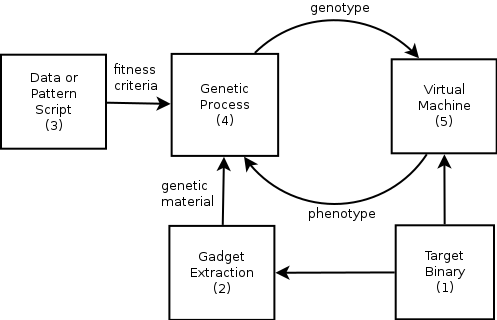
\includegraphics[width=.9\linewidth]{../images/birdseye.png}
\caption{\label{fig:org0448df7}
A bird's eye view of \gls{roper}. Algorithm \ref{alg:rop-sweep} takes us from (1) to (2); algorithm \ref{alg:initpop} takes us from (2) to (4); algorithms \ref{alg:evolve} and \ref{alg:evalgen} cycles us between (4) and (5), and fairly standard loading and parsing algorithms join (3) up with (4) and (1) with (5).}
\end{figure}


\begin{algorithm}
\caption{Population Initialization}
\label{alg:initpop}
\begin{algorithmic}[1]
\REQUIRE $\varepsilon$, ELF binary of the process to be attacked
\REQUIRE $\pi$, the problem set specification
\REQUIRE $n$, the desired population size
\REQUIRE $\iota$, a pool of dwords (random, or informed by domain-specific knowledge)
\REQUIRE $(\frak{R},s)$, a pseudo-random number generator and seed
\STATE {code segments, data segments $\gets$ parse($\varepsilon$)}
\STATE {add interesting pointers from data segments to $\iota$}
\STATE {$\gamma \gets$ harvest-gadgets(code segments)} \COMMENT {see \ref{alg:rop-sweep}}
\STATE {$\Pi \gets$ empty-vector($n$)}
\STATE {$\frak{R}$ $\gets$ seed($\frak{R},s$)}
\FOR {$x \gets 1 $ \TO $n$}
\STATE {$\frak{R}$, $\Pi_x$ $\gets$ 
        make a random chain from elements of $\gamma$ and $\iota$, using $\mathfrak{R}$}
\label{alg:initpop:line:spawn-individual}
\ENDFOR
\RETURN population
\end{algorithmic}
\end{algorithm}


\begin{algorithm}
\caption{Genotype Evaluation (Ontogenesis)}
\label{alg:evalgen}
\begin{algorithmic}[1]
\REQUIRE $E$, the CPU emulator
\REQUIRE $IO: [(in, out, weight)]$, the input/output rules for the problem set
\REQUIRE $\varphi$: a task-specific fitness function, mapping CPU states to floats
\REQUIRE \texttt{SENTINEL}: uint, a fixed-width integer constant (0, e.g.)
\REQUIRE $\mu$: $\mathbb{N}$, the maximum number of execution steps permitted
\REQUIRE acc: $\mathbb{F} \times \mathbb{F} \rightarrow \mathbb{F}$, an accumulator function for fitness scores (running average, for example)
\REQUIRE $\Gamma$, the genotype to be evaluated
\STATE {$\sigma \gets $ serialize($\Gamma$) $\cup$ [SENTINEL]}  \COMMENT {\emph{into a stack of bitvectors}}
\STATE {accumulator $\gets$ ()}
\FORALL {case in $IO$}
\STATE {$E$ $\gets$ prime $E$ with case.in}
\STATE {$E$ $\gets$ load $\sigma$ into stack memory of $E$}
\STATE {$E$ $\gets$ exec($E$, \texttt{"POP PC, SP"})} \COMMENT {\emph{pop stack into program counter}} 
\STATE {$i \gets 0$}
\WHILE {$i < \mu$ \AND program-counter($E$) $\neq$ SENTINEL \AND in-legal-state($E$)}
\STATE {$E \gets$ step($E$)} \COMMENT {\emph{fetch instruction at }\texttt{PC}\emph{ and execute}}
\STATE {$i \gets i+1$}
\ENDWHILE
\COMMENT {We can think of the state of $E$ as the `base phenotype'}
\STATE {fitness $\gets$ acc(fitness, case.weight, $\varphi(E, \text{case})$}
\STATE {$E$ $\gets$ reset($E$)}
\ENDFOR 
\RETURN {fitness}
\end{algorithmic}
\end{algorithm}

\begin{algorithm}
\caption{Evolve Population (Tournament Selection)}
\label{alg:evolve}
\begin{algorithmic}[1]
\REQUIRE $\Pi$, the population \COMMENT {\emph{as initialized by Algorithm~\ref{alg:initpop}}}
\REQUIRE $E$, the CPU emulator
\REQUIRE $\Omega: \Pi \rightarrow \mathbb{B} $, the stop condition (predicate over $\Pi$)
\REQUIRE $\Sigma$, the problem set (labelled exemplars for classification, patterns to match, game states to respond to, etc. -- the precise nature of this set is task-specific)
\REQUIRE $(\frak{R}, s)$, a PRNG and seed
\REQUIRE $n$, the number of individuals competing in each selection tournament
\STATE {$\frak{R}$ $\gets$ seed($\frak{R}, s$)}
\REPEAT
\STATE {$\frak{R}$, candidates $\gets$ using $\frak{R}$, pick $n$ from $\Pi$}
\label{alg:evolve:line:candidates}
\STATE {$\Phi \gets $ empty list of (float, genotype) pairs}
\FOR {$\Gamma$ in candidates} 
\STATE {$\Gamma_\textit{fitness}$ $\gets$ evaluate-genotype($\Gamma, \Sigma, E$)}
\COMMENT {\emph{Algorithm~\ref{alg:evalgen}}}
\ENDFOR
\STATE {$\Phi \gets$ sort($\Phi$, by \emph{fitness})}
\STATE {victors $\gets$ take $m$ from $\Phi$}
\STATE {vanquished  $\gets$ take $k$ of reverse($\Phi$)}
\STATE {$\frak{R}, \textrm{offspring}_{1\dots k} \gets \textit{breed}(\frak{R}, k, \textrm{victors})$}
\label{alg:evolve:line:breed}
\STATE {$\Pi \gets [\textrm{vanquished/offspring}]\Pi$} \COMMENT {replace vanquished with offspring}
\UNTIL {$\Omega(\Pi) = \TRUE$}
\STATE {champion $\gets$ head(sort($\Pi$, by \textit{fitness}))}
\RETURN {champion}
\end{algorithmic}
\end{algorithm}

\begin{figure}[htbp]
\centering
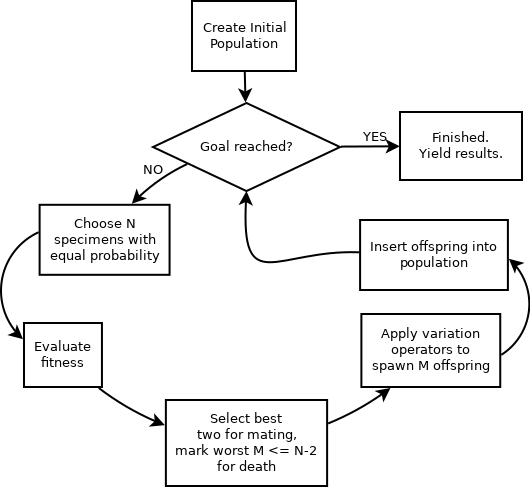
\includegraphics[width=.9\linewidth]{../images/tournament_black.png}
\caption{\label{fig:orgc27bffc}
High-level overview of the tournament selection algorithm}
\end{figure}


Algorithms \ref{alg:initpop}, \ref{alg:evalgen}, and \ref{alg:evolve}
furnish a bird's eye view of \gls{roper}, abstracting away from questions of
implementation, and streamlining away various bits of functionality
aimed at optimization, bookkeeping, and fine-tuning.

\gls{roper} begins with the analysis of an executable binary file (either an
application or a library). For the time being, we are restricting
ourselves to binaries targetting the 32-bit \gls{armv7} architecture, in ELF
format, but there is nothing essential about this restriction, and
\gls{roper} could easily be extended to handed a variety of hardware
platforms and executable formats, if desired. It harvests as many viable
ROP gadgets as it can from the file (within parameterizable limits), by 
means of a linear sweep search, walking backwards through the file's
executable \texttt{.text} section until it hits a return instruction, and then
walking further backwards until it reaches an instruction that would
prevent the execution flow from reaching the return. This isn't the
most thorough or exacting technique for finding gadgets, and a wider
variety of potentially usable gadgets can be uncovered by means of
a constraint-solving algorithm, which is able to detect stack-controllable
indirect jumps other exploitable control-flow artefacts as well. (We experiment
with such an approach in \gls{roper} II, which is still in progress at the time of
writing.) A linear sweep nevertheless suffices to provide us with a fairly
generous number of gadgets for our purposes, and has the advantage of being
both simple and efficient.

The addresses of these gadgets, together with a pool of potentially useful
immediate integer values and data pointers, which can be supplied by the
user, or inferred from the specification of the problem set, supply us with
the primtive genetic units from which the first genotypes in the population will
be composed. With no more abuse of terminology than is customary in evolutionary
computation, we can call this the ``gene pool'' of the population. It should
nevertheless be noted that the biological concept of \emph{gene} presupposes many
structural constraints that have, as of yet, no parallel in our system.

The initial population, as yielded by Algorithm \ref{alg:initpop}, is
little more than an array of variable-length vectors of machine words
 (32-bits, so long as we are restricting ourselves to the
\gls{armv7}, but, again, this restriction matters little so far as the
system's algorithmic structure is concerned). The length of the
initial individuals is left parameterizable, but is upper-bounded by
the amount of stack memory that will be available in the target
process for our attacks to write to. We will complicate this structure
somewhat, in \S \ref{org8dbfd06}, but it remains a useful
simplification. The words making up each individual may be either
gadget addresses or other integers, which the individual's gadgets may
use to populate registers \emph{other} than \gls{pc}. To stack the deck a little,
we may inject various potentially useful integers into the primordial ooze
from which the initial population is spawned. The selection of these depends
on the problem set, and on domain-specific knowledge (or hunches), and they
may include both words intended to be used as immediate integer values, and
words intended to be used as pointers to potentially useful information in
the data segments. 

The main loop, outlined in Algorithm \ref{alg:evolve} and figure \ref{fig:orgc27bffc},
is built around a well-known and widely used genetic programming algorithm
called ``tournament selection''. On each iteration of the loop, \(n\) (typically 4)
distinct candidate genotypes are chosen from the population, with equal
probability. Each is then mapped to its phenotype (its behavioural profile in
the emulated \gls{cpu}), and its fitness evaluated (by applying the fitness
function to that profile). The \(m\) (typically 2) candidates with the best
fitness are selected for reproduction, while the least-fit \(k\) candidates are
culled from the population.

The genotypes selected for reproduction are then passed to our genetic
operators, which will return \(k\) offspring, who will replace the least-fit \(k\)
candidates in the tournament. In the genetic programming literature, these
operators are often referred to as the ``variation operators'', as they ``define the
manner in which the system moves through the space of possible solutions''
(\cite{banzhaf98}, 144). In \gls{roper}, our genetic operators comprise a
single-point crossover function, which maps a pair of parents into a pair of
offspring, and a mutation operator, which maps a single genotype into a variant
thereof. The internals of these operators are detailed in \S
\ref{orgcf8d05c}.

This loop continues until the halting conditions are satisfied. These are most
often set either to a maximum number of iterations, or the attainment of a set
degree of fitness by the population's fittest specimen.

In the following sections, we will explain the finer-grained design decisions
involved in implementing the algorithms specified above. 

In the following sections, I will unfold and justify the decisions that went into
implementing the algorithms surveyed in \S \ref{org79f56c8}.
We can begin with the representation of the genotypes constructed by
the \textbf{spawn-individual()} algorithm, called on line
\ref{alg:initpop:line:spawn-individual} of Algorithm \ref{alg:initpop}.

\section{Gadget Extraction}
\label{sec:org5a86b4d}
\label{org59df2db}

\begin{figure}[htbp]
\centering
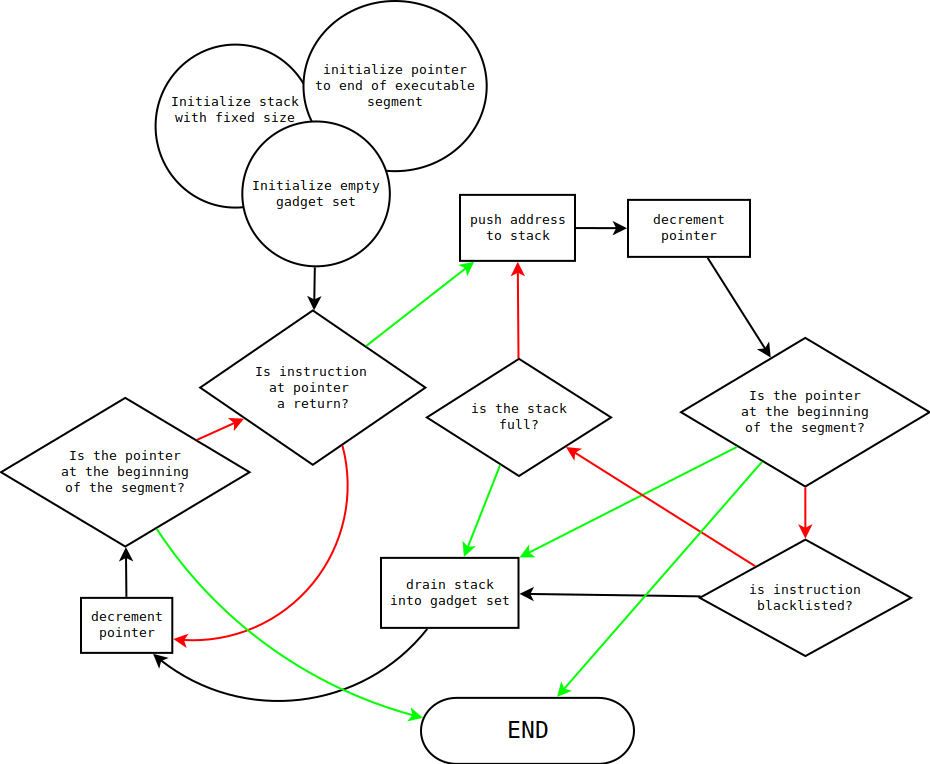
\includegraphics[width=.9\linewidth]{../images/gadget-harvest-dark.png}
\caption{\label{fig:orgd8dd461}
Harvesting gadgets from a \gls{risc} executable segment.}
\end{figure}

Since the aim of \gls{roper} is to foster the evolution of ROP chains, we 
must begin by supplying the engine with a sufficient pool of gadgets, 
harvested from the target executable. 
  \footnote{See \S \ref{org46997d9} for a sustained explanation of how return-oriented
  programming works, and an explanation of the concept of 'gadget'.}

There are several ways that this can be done, but the simplest is just to
scan the executable for a subset of easily recognizable 'gadgets' using a
linear sweep algorithm, shown in Algorithm \ref{alg:rop-sweep} and diagrammed 
in figure \ref{fig:orgd8dd461}. Since we are
dealing only with a RISC instruction set architecture here, we can avoid 
several complexities in our gadget search that we would need to grapple with
were we adapting \gls{roper} to handle CISC instruction sets (such as the x86 and
its ilk) as well. The instructions of a RISC ISA are all of equal length
(with a certain exceptions, and assumping the mode fixed), and so if a
sequence of bytes beginning at address \(i\) is parsed as instruction \(X\)
when beginning the parse \emph{from} \(i\), then it will also be parsed as \(X\)
when beginning the parse from some \(j < i\). To put it another way, the
list of RISC instructions parsed from bytevector \(\mathbf{C}\), beginning
at address \(i\), extends \emph{monotonically} with each decrement of \(i\).
In practical terms, this means that an instruction that looks like a
return from far away will still look like a return by the time you've parsed your
way up to it. This is very different from what we encounter with CISC ISAs,
where the length of instructions is variable, and instructions are not aligned.
Suppose we had the string \texttt{"aabbcc"} of bytes. Suppose that \texttt{aa} parses to
\(\alpha\), \texttt{ab} parses to \(\beta\), \texttt{bb} parses to \(\tau\), \texttt{cc} parses to \(\delta\) and
\texttt{bcc} parses to \(\gamma\). If we begin the parse from the beginning of the string,
we get \(\alpha \tau \delta\). But if we increment our cursor one byte forward
before parsing, then our parse yields \(\beta \gamma\), with \(\delta\) nowhere
to be seen. In order to adapt our gadget harvesting algorithm to CISC ISAs,
therefore, we would have to continually check to ensure that the \textbf{return}
instruction spotted at line \ref{alg:rop-sweep:line:see-ret} of
Algorithm \ref{alg:rop-sweep} is still parseable as a return, and still reachable, from
the address indicated by \(i\) on line \ref{alg:rop-sweep:line:storegadget}. This
would increase the complexity of the algorithm substantially. 

Fortunately, for the time being, we are concerned only with the two main
instruction sets of the \gls{armv7}: the \emph{arm} instruction set, which is aligned
to four-byte intervals, and the \emph{thumb} instruction set, which is aligned to
two-byte intervals. There is no essential difference in the functionality of
these two instruction sets -- both are Turing-complete, and entire operating
systems can get along just fine using one or the other. What the difference in
modes offers are resources for navigating various time/space trade-offs: arm
mode offers greater internal parallelism, semantic nuances (every instruction
offers conditional variants, and ``free'' bitshifting), and register selection,
but its larger instructions make its use more memory intensive and slower in
ROM, while thumb mode offers greater instruction-per-byte density, and may be
favoured in situations where space is at a premium, or where the code bus has
limited bandwidth (the Game Boy Advance, for instance, almost exclusively uses
thumb mode, for this reason \cite{gbaguy} \cite{coranac}). In crafting \gls{rop}
payloads, we're not particularly invested in these costs and benefits, but the
added semantic variety resulting from the ability to switch between \gls{arm} and
\gls{thumb} mode, as we like, and the possibility of parsing arbitrary
instructions in both modes -- regardless of which was \emph{intended} -- is a boon to
the \gls{rop} chainer. A sufficient supply of gadgets can usually be found by
passing our extraction algorithm twice over the executable segments of our
target binary, gathering a pool of both \emph{arm} and \emph{thumb} gadgets. Since the
least significant bit of an instruction address is invariably 0, for this ISA,
the \gls{arm} \gls{cpu} uses this bit to distinguish between \emph{arm} mode and \emph{thumb}
mode. We therefore increment the address of each of our freshly harvested thumb
gadgets by 1.



\begin{algorithm}
\caption{Linear sweep algorithm for gadget extraction.}
\label{alg:rop-sweep}
\begin{algorithmic}[1]
\REQUIRE {$\mathbf{C}$: a contiguous vector of bytes representing instructions}
\REQUIRE {$\ulcorner{X_j}\urcorner: [\mathbf{byte}] \rightarrow \mathbb{N} \rightarrow \textrm{inst}|\Lambda$,
a parsing function, from byte-vectors $X$ and indices $j$ to instructions, or $\Lambda$ in
case of unparseable bytes.}
\REQUIRE {$\rho: \textrm{inst} \rightarrow \mathbb{B}$, predicate to recognize returns}
\REQUIRE {$\varphi: \textrm{inst} \rightarrow \mathbb{B}$, predicate to recognize control instructions,
with $\forall(x)~\rho(x)\Rightarrow\varphi(x)$, but not necessarily the converse. $\varphi$ should
also return \textbf{true} for $\Lambda$ (signalling unparseable bytes).}
\REQUIRE {$\delta$: positive integer,  offset of base virtual address for $\mathbf{C}$}
\STATE {$\Gamma \gets$ empty stack of integers}
\STATE {$i \gets $ length($\mathbf{C}$)}
\WHILE {$i > 0$}
  \STATE {$i \gets i - 1$}
  \IF {$\rho(\ulcorner\mathbf{C}_{i+1}\urcorner)$} \label{alg:rop-sweep:line:see-ret}
    \WHILE {$\neg \varphi(\ulcorner\mathbf{C}_i\urcorner)$ \AND $i > 0$}
      \STATE {push $i$ onto $\Gamma$} \label{alg:rop-sweep:line:storegadget}
      \STATE {$i \gets i - \textrm{length}(\ulcorner\mathbf{C}_i\urcorner)$}
    \ENDWHILE
  \ENDIF 
 \ENDWHILE
\STATE {$\Gamma^\star \gets \textrm{map~}(\lambda x. \delta + x) \textrm{ over } \Gamma$}      
\RETURN {$\Gamma^\star$}
\end{algorithmic}
\end{algorithm}

\section{Genotype Representation: Gadgets, Clumps, and Chains}
\label{sec:org530f933}
\label{org8dbfd06}
\label{sec:clumps}

From a certain perspective -- that of the evaluation engine -- the individual
genotypes of the population are little more than bare ROP-chain payloads:
vectors of 32-bit words, each of which is either a pointer into the executable
memory of the host process, or raw data (the former being a subtype of the
latter, of course). The view afforded to the genetic operators, and to the
initial spawning algorithm, exposes slightly more structural complexity,
which is introduced in response to the following problem:

In the set of 32-bit integers (\(\texttt{0x100000000}\) in all), the subset representing
the set of pointers into the executable memory segments of a given ELF file
tends to be rather small: in the case of \texttt{tomato-RT-N18U-httpd}, an HTTP
server that ships with a version of the Tomato firmware for certain \gls{arm}
routers, which we will be using for a few of the experiments that follow,
we can see that only \(\texttt{0x1873c} + \texttt{0xc0} = \texttt{0x187ec}\) bytes are mapped to executable
memory. Now, the \gls{armv7} \gls{cpu} is capable of running in two different modes, each
with their own instruction set: \emph{arm} mode, which requires the instructions to
be aligned to 4-byte units, and \emph{thumb} mode, which demands only a 2-byte alignment
of instructions. Since the least significant bit in a dword can therefore not be
used to differentiate between instruction addresses, the \gls{armv7} \gls{cpu} uses it to
distinguish between the two modes: any address \(a\) whose least significant bit is 1
(i.e., any odd-valued address) is dereferenced to a thumb instruction
at address \(a \oplus 1\) (rounding down to the nearest even address). 
This gives us a total of \(\frac{\texttt{0x187ec}}{4} + \frac{\texttt{0x187ec}}{2} = \texttt{0x125f1}\) valid
executable pointers -- which, roughly, means that only one in fifty-thousand
of integers between \texttt{0x00000000} and \texttt{0xFFFFFFFF} can be dereferenced to executable
memory in a the ELF executable in question -- a ratio that is seldom increased
by more than one or two orders of magnitude, even when dealing with large,
statically linked ELF binaries.
  \footnote{There's a fair bit of handwaving, here, when referring to a 'typical' ELF 
  executable -- obviously the size of the executable can vary. We're also restricting
  ourselves to the executable memory mapped in the file of a \emph{dynamically linked}
  executable here, ignoring the addresses that may dereference to executable addresses
  where dynamically loaded libraries might be mapped.}

\begin{table}
\scriptsize
\caption{Program Headers of a Typical ELF Executable}
\label{tab:readelf-tomato}
\hrule
\begin{verbatim}
$ readelf --program-headers tomato-RT-N18U-httpd

Elf file type is EXEC (Executable file)
Entry point 0xa998
There are 6 program headers, starting at offset 52

Program Headers:
  Type           Offset   VirtAddr   PhysAddr   FileSiz MemSiz  Flg Align
  PHDR           0x000034 0x00008034 0x00008034 0x000c0 0x000c0 R E 0x4
  INTERP         0x0000f4 0x000080f4 0x000080f4 0x00014 0x00014 R   0x1
      [Requesting program interpreter: /lib/ld-uClibc.so.0]
  LOAD           0x000000 0x00008000 0x00008000 0x1873c 0x1873c R E 0x8000
  LOAD           0x01873c 0x0002873c 0x0002873c 0x0040c 0x005c8 RW  0x8000
  DYNAMIC        0x018748 0x00028748 0x00028748 0x00118 0x00118 RW  0x4
  GNU_STACK      0x000000 0x00000000 0x00000000 0x00000 0x00000 RW  0x4

 Section to Segment mapping:
  Segment Sections...
   00     
   01     .interp 
   02     .interp .hash .dynsym .dynstr .gnu.version .gnu.version_r .rel.dyn 
          .rel.plt .init .plt .text .fini .rodata .eh_frame 
   03     .init_array .fini_array .jcr .dynamic .got .data .bss 
   04     .dynamic 
   05     
\end{verbatim}
\hrule
\end{table}

This means that if we allow the integers composing the genotypes of our
initial population to be randomly selected from the entire 32-bit range,
only a tiny fraction of those integers will dereference to any meaningful
executable addresses in the code -- let alone useful gadget addresses.
Restricting the pool of integers sampled to the set of valid executable 
pointers, let alone gadget addresses, however, may deprive
the population of useful numerical values. 

The execution of these individuals, after all, will be driven by return
instructions, and these, in \gls{arm} machine code, are most often implemented as
multi-pops, which pop an address from the stack into the program counter, while
simultaneously popping a variable number of dwords into other, general-purpose
registers. This means that each \texttt{return} -- each ``tick'' of the ROP state-machine
-- not only steers the control flow of our machine, sending it to a new gadget,
but the data flow as well, furnishing each gadget with a handful (between zero
and a dozen) of numerical values, to use internally. We don't necessarily want
to restrict these numerical resources to the range of gadget pointers -- it would
be better, in fact, if we could tailor the pool of ``potentially useful'' numerical
values to a set of integers (including, perhaps, data pointers) that seems suited
to the problem set at hand. 

This suggests a potentially useful structural constraint that we can
impose on the genotypes, to increase the likelihood that they will be found
useful for the problem space at hand, and greatly increase the probability that
\texttt{.text} pointers will be popped into \gls{pc}, while other 
integers land predominantly in general-purpose registers.
To do this, we calculate the distance the stack pointer will shift
when each gadget executes, the \gls{spd} of \(g\) or \(\gls{spd}(g)\), and then clump together
each gadget pointer \(g\) with a vector of \(\gls{spd}(g)-1\) non-gadget
values. Consider, for example, the instruction,
\[\mathtt{LDMIA!~~~~SP,~~\{R0, R7, R9, PC\}}\]
which pops the stack into registers \texttt{R0}, \texttt{R7}, \texttt{R9}, and \gls{pc}, in sequence,
``returning'' the program counter to the address represented by the fourth dword
on the stack, while at the same time populating three general purpose registers
with the stack's first three dwords. This instruction has a \(\gls{spd}\)
of 4. For a gadget \(g\), we define \(\gls{spd}(g)\) as 
$$\gls{spd}(\pi) = \sum_{i\in \pi} \gls{spd}{i}$$
for some control path \(\pi\) in \(g\) that reaches the return. In practice,
we choose our initial pool of gadgets in such a way that each contains only a basic
block of code, with control flow entirely in the hands of the return instruction
that terminates it, so that the choice of \(\pi\) is unique for each \(g\). If this
condition is relaxed, we suggest generating \(n\) distinct clumps for each
distinct member of \(\{\gls{spd}(\pi)|\pi \textit{ is a control path in } g\}\).
Exactitude isn't strictly necessary, here, however -- as we'll see, the
evolutionary process that follows is robust enough to handle a fairly large
number of gadgets with miscalculated \(\gls{spd}\) values. A good rule of thumb,
here, is that when the approximation of \(\gls{spd}(g)\) is left inexact, in the
interest of efficiency, dump several options into the pool, and let natural
selection sort them out.

Given a gadget entry point address \(\addr{g}\), a ``clump'' around \(g\) can now be
assembled by taking a stack of \(\gls{spd}(g)-1\) arbitrary values, and pushing
\(\addr{g}\) on top of it. By the time \(g\) has run to completion, it will have popped
\(\gls{spd}(g)\) values from the process stack. The first \(\gls{spd}-1\) of
these will populate the general purpose registers of the machine, and the
\({\gls{spd}}^{\textit{th}}\) will pop the entry point of the \emph{next} gadget,
\(g'\), into \texttt{pc}. That entry point, \(\addr{g'}\) will be found at the top of the
next clump in the sequence that makes up the genotype.\footnote{\gls{roper} also handles gadgets that end in a different form of
  return: a pair of instructions that populates a series of registers
  from the stack, followed by an instruction that copies that address
  from one of those registers to \texttt{pc}. In these instances,
  \(\Delta{SP}(g)\) and the offset of the next gadget from \(g\) are
  distinct. But this is a complication that we don't need to dwell on
  here.}

As explained in \S \ref{org63bfd56}, it is often helpful to think of
each gadget as an instruction in a virtual machine -- an emergent machine,
supervening on the host's native instruction set architecture. What we're
calling a clump here maps onto this concept of ``instruction'', but with a
slight displacement: the gadget address can be seen as something
like an ``opcode'' for the \gls{rovm}, and the immediate values in each clump
can be seen as operands -- \emph{but operands of the next instruction}, not of
the instruction whose opcode is represented by their own clump's gadget
pointer.

When the initial population is generated, we take a pool of gadget pointers, 
harvested from the target binary (see \S \ref{org59df2db}), and a
pool of integers and data pointers, supplied by the user as part of the problem
specification. We then form clumps, as described above, using randomly chosen
elements of these two pools, as needed. The clumps are then assembled into 
variable length chains (with the minimum and maximum allowed lengths being
parameterized by the user), which gives us our genotype representation. The
internals of this algorithm are detailed in Algorithm~\ref{alg:spawn}.

\begin{algorithm}
\caption{Spawning an Initial Individual}
\label{alg:spawn}
\begin{algorithmic}[1]
\REQUIRE $\mathbf{G}: [\![\mathbb{N}^{\,32}]\!]$, a set of gadget pointers
\REQUIRE $\mathbf{P}: [\![\mathbb{N}^{\,32}]\!]$, a set of integers and data pointers
\REQUIRE $(\mathfrak{R}, s)$: a PRNG and seed
\REQUIRE $(min, max): (\mathbb{N}, \mathbb{N})$, minimum and maximum genotype lengths
\STATE {$\Gamma \gets $ empty stack of clumps} \COMMENT{\emph{the genotype representation}}
\STATE {$\mathfrak{R} \gets $ seed$(\mathfrak{R},s)$}
\STATE {$n, \mathfrak{R} \gets $ random-int($\mathfrak{R}$, min, max)}
\FOR {$i \gets 0$ to $n$}
  \STATE {$\addr{g}, \mathfrak{R} \gets $ choose$(\mathfrak{R}, \mathbf{G})$}
  \STATE {$C \gets $ empty stack of $\mathbb{N}^{\,32}$}
  \STATE {$\delta \gets \gls{spd}(g)$}
  \COMMENT {\emph{cf. sec. \ref{sec:clumps} for def. of $\gls{spd}$}}
    \FOR {$j \gets 0$ to $\delta$} 
      \STATE {$p, \mathfrak{R} \gets $ choose$(\mathfrak{R}, \mathbf{P})$}
      \STATE {push $p$ onto $C$}
    \ENDFOR
    \STATE {push $\addr{g}$ onto $C$}
  \STATE {push $C$ onto $\Gamma$}
\ENDFOR
\RETURN {$\Gamma$}
\end{algorithmic}
\end{algorithm}

\section{Genetic Operators}
\label{sec:org8f6f8a8}
\label{orgcf8d05c} 

In order for our population of loosely structured but otherwise random
ROP chains to explore the vast and uncharted space of possible combinations
and (on the side of phenotypes) their associated behaviours, we need a
means of moving from a given subset of our population to ``similar'' genotypes
in the neighbourhood of that subset, which may not yet belong to the population.
This is accomplished by the genetic operators, which allow our population to
search the genotype space through reproduction and variation.

\gls{roper} makes use of two such operators: a crossover operator, which operates 
on genotypes as lists of clumps, and a mutation operator, which operates on
clumps internally. 

\subsection{Mutation}
\label{sec:org11f1f7d}
     \label{org0b80a57}
The mutation operator selects, randomly, from a set of transformations,
which it then applies to one or more words contained in one or more randomly
selected clumps. The choice of operation is constrained by the word slot being
operated on: the word that is (probabilistically) fated to be loaded into the
instruction pointer isn't subject to the same range of modifications that the
other words in the clump are. The reason for this is that the performance of an
individual will, in general, be more sensitive to modifications to its gadget
pointers than to its immediate values, and so it makes sense to afford the
mutation operator a greater degree of freedom when dealing with a value that is
unlikely to be used to directly control the instruction pointer. It is
relatively safe to increment or decrement a pointer by a word size or two, but
almost always hazardous to negate or shift it, for example.

The rest of the words in the clump can be mutated much more freely. The
operations currently available include:

\begin{enumerate}
\item arithmetically, by applying either numerical operations such as addition and
subtraction;
\item bitwise operations, such as shifts, rotations, sums, and products by
a randomly selected constant value;
\item the pointer operations of dereference (interpreting a value as a pointer,
when possible, and replacing it with the value found at the corresponding
address in the process's memory) and indirection (the somewhat more
costly (\(O(n)\) over the size \(n\) of the memory space) operation of
searching through memory for an instance of the value, and replacing
it with a pointer that dereferences to it). When a value cannot be
dereferenced as a pointer, or a pointer to a word cannot be found in
memory, the operation collapses to the identity function;[fn::
Putting \(\&\) for raw indirection and \(*\) for raw dereference, as in C,
our pointer operators \(\&'\) and \(*'\) are defined as endomorphisms in
\(\mathbb{2}^{32}\), where \(\&'(x) = \&x\) when \((\exists y) *y = \&x\),
and \(\&'(x) = x\) otherwise. \(*'\) is the dual of \(\&'\). Unlike the
familiar C operators, our pointer mutations therefore have algebraic
closure.
\item a permuation operation, by which two randomly selected machine words in a clump exchange
places;
\item a combination of 3 and 4, where two randomly selected words in a clump are chosen,
and one is replaced with their bitwise sum, the other with their bitwise product;
\end{enumerate}

What the four mutation operations have in common is that
they share a certain minmal algebraic structure. Within each set, each
operation -- which, formally, is a endomorphism over \(\mathbf{[2^{32}]}\) --
has an inverse: 
\[
(\forall M\in S)(\forall x)(\exists y) M(x) = y \Rightarrow 
(\exists M'\in S) M'(y) = x
\]
and an identity:
\[
(\forall M\in S)(\exists x) M(x) = x
\]
What this means is that over each set of mutation operators -- and
therefore over their union -- the concatenation or succession their
application forms a cyclic group.\footnote{The proof is left as an exercise for the author.}

In practical terms, this is a generally beneficial property for genetic
operators to possess: all else being equal, they should be designed with
an eye towards neutrality with respect to an arbitrary choice of fitness
functions. By ensuring that the mutation operators are involutive, or, more
generally, that they form a cyclic concatenation group, involution just being
the smallest nontrivial form of such a structure, with a cycle of two, we
(imperfectly) guard against a situation where they ratchet the population into a
small corner of the genotypic (and, consequently, the phenotypic) landscape,
\emph{independent of the fitness function}. (Identity is less significant, in this
context, and is introduced into the mutation operators only
as a way of ensuring closure.) Ratcheting occurs when the genetic
operators are not properly balanced. In the situation where the algebra defined
by concatenation over the mutation operators does \emph{not} form a cyclic group --
when there is ``no way back'' from some mutation \(M\) by any succession of further
mutations -- ratcheting is inevitable. This problem is distinct from, but
related to, the problem of genetic drift, which it exacerbates. Involutive pairs
of operators, selected with equal probability, provide some safeguard against
this. The \emph{ideal}, in some sense, would be to select genetic operators that
would engender an \emph{ergodic} system under a null fitness function:\footnote{Thanks to
Andrea Shepard for this insight.} one whose behaviour is evenly distributed
over the probability landscape it inhabits. In practice, even with fitness
anulled, evolutionary systems rarely exibit such regularity, which has some very
interesting effects on the paths that evolution pursues. We will study some of
these consequences in Chapter \ref{org8167c36}.


\subsection{Crossover}
\label{sec:orge8ce370}
\label{orgdda015b} 

At a slightly higher structural level, the reproduction
algorithm may apply a crossover operation to the list of clumps, taking the
clumps as opaque units.

I chose single-point crossover over two-point or uniform crossover to favour
what I judged to be the most likely form for gene linkage to take in this
context: A single gadget can transform the \gls{cpu} context in fairly complex
ways, since it may include any number of architectural instructions. The
prevalence of multipop returns in \gls{arm} code further increase the odds that
the work performed by a gadget \(g\) will be clobbered by a subsequent gadget
\(g'\), and this risk increases monotonically as we move down the chain from \(g\).
This means that adjacent gadgets are more likely to achieve a combined,
fitness-relevant effect, than non-adjacent gadgets. Lacking any reason to
complicate things further, we restricted the number of parents involved in each
mating event to two. \footnote{One of the limitations of \gls{roper} is that the mating
algorithm, and the genetic variation operators in general, are assumed fixed. In
\gls{roper} II, we will experiment with a technique for opening this, too, to
genetic exploration and selective pressure, which Lee Spector calls
``autoconstructive evolution''.}


In single-point crossover between two genotypes, \(\mu\) and \(\varphi\), we
randomly select a link index \(\mu_i\) where \(\mu_i < |\mu|\), and \(\varphi_i\)
where \(\varphi_i < |\varphi|\). We then form one child whose first \(\mu_i\) genes
are taken from the beginning of \(\mu\), and whose remaining genes are taken from
the end of \(\varphi_{\mu_i\dots}\), and another child using the complementary
choice of genes. The only modification I make to this well-known algorithm, in
\gls{roper}, is to weight the choices of \(\mu_i\) and \(\varphi_i\), using a
parameter we call ``fragility'', whose calculation I explain in \S
\ref{org7016026}. The details of the algorithm itself can be found in
\ref{alg:crossover}.

\begin{algorithm}
\caption{Single-Point Crossover, with Fragility} \label{alg:crossover}
\begin{algorithmic}[1]

\REQUIRE $(\vec{\mu}, \vec{\varphi})$: ([\![ \textbf{clump} ]\!], [\![\textbf{clump} ]\!]), the parental genotypes 
\REQUIRE \emph{Fragility}: [\![\textbf{clump} ]\!] $\times$ [\![ \textbf{clump} ]\!] $\times$ lineage $\to \mathbb{F}$ 
\REQUIRE $(\mathfrak{R}, s)$: a PRNG and seed \REQUIRE $n$: $\mathbb{N}$, brood size


\STATE {$\mathfrak{R} \gets \textit{seed}(\mathfrak{R}, s)$} 
\STATE
{splice-points $\gets ()$} \COMMENT {the indices at which the parental genes
will be recombined} \FOR {$\vec{\alpha} \in (\vec{\mu }, \vec{\varphi})$} 
\STATE
{$t \gets \sum_{\alpha \in \vec{\alpha}} 1.0 - \textit{Fragilty}(\alpha)$}

\STATE {$p, \mathfrak{R} \gets \textit{random-float}(\mathfrak{R}, t)$} \COMMENT
{$p$ is more likely to fall on a highly fragile link} 
\STATE {$x \gets 0$}

\STATE {$i \gets 0$} \WHILE {$x < p$} 
\STATE {$x \gets x +
\textit{Fragility}(\alpha_i)$} 
\STATE {$i \gets i + 1$} \ENDWHILE 
\STATE {push
$(\vec{\alpha}, i)$ onto splice-points} \ENDFOR 
\STATE {\textbf{let} $\mu^a,
\mu^b = $ split $\mu$ at splice-points.lookup($\mu$)} 
\STATE {\textbf{let}
$\varphi^b, \varphi^a = \textit{split} \varphi \textit{at}
\textit{splice-points.lookup}(\varphi)$} 
\STATE {\textbf{let} $\chi^a = \mu^a
\cup \varphi^a$} 

\STATE {\textbf{let} $\chi^b = \varphi^b \cup \mu^b$} \RETURN
{$\chi^a, \chi^b$} \COMMENT {the offspring}
\end{algorithmic} 
\end{algorithm}

Crossover, so defined, has certain algebraic properties that allow it
to interact harmoniously with the forms of mutation specified in 
Section \ref{org0b80a57}. If we abstract away from the information loss
enabled by the possibility of dropping of genes with low link fitness, a
probabilistic parameter that can be tuned, in \gls{roper}, then, under the
assumption of a maximum genome length -- an assumption that holds in \gls{roper},
and which is imposed quite naturally by the practical limits of stack space in
the target process -- the crossover function, too, can be shown to form a cyclic group
under concatenation. Let \(a\) and \(b\) be two chains selected for crossover, and 
\(C(a,b)\) the set of \emph{possible} offspring that may emerge from their mating. If
we restrict the splice index of the crossover to be nonzero, then \(a,b \not \in C(a,b)\).
But if we then take the set \(\mathbb{C}(C(a,b))\) of all possible offspring resulting
from an inbreeding of members of \(C(a,b)\), then we \emph{do} find that both \(a\) and \(b\)
appear in this set. There is provable possibility for a chain, identified only by
its packed composition and without considering its genealogical metadata, to be its
own grandpa. 

Crossover is therefore associative, and since the crossover operation is symmetrically
defined -- one of the two offspring that are \emph{actually} produced by a mating of \(a\) 
and \(b\) will begin with clumps from \(a\), the other with clumps from \(b\), with the other
parent providing the tail -- we can show that the mutation operators defined in
Section \ref{org0b80a57} commute with and distribute over crossover, if we consider
them as functions that take probability distributions of offspring as their codomain. 

This is still some distance from rigorously establishing that \gls{roper}'s populations
will, asymptotically, approximate an ergodic system -- a system where any states that
are reachable at the outset remain reachable, by an arbitrarily long but
finite path of genetic operations, from any point in that system's evolution -- but
it does at least establish the plausibility of ergodicity. In practice, however,
convergence and evolutionary deadends may remain commonplace, and it is only a very
slight reassurance to know that such states of affairs are not irreversible or 
eternal, in principle.\footnote{For a rigorous discussion of ergodicity in genetic algorithms, as a consequence of the algebraic structure of the genetic operators -- and, in particular, of the commutativity of mutation and crossover -- see \cite{schmitt01}.}


\subsubsection{Fragility and Gene Linkage}
\label{sec:org97bba6e}
\label{org7016026}

As a way to encourage the formation of complex 'building blocks' -- sequences of
clumps that tend to improve fitness when occurring together in a chain -- we
weight the random choice of the crossover points \(\mu_i\) and \(\varphi_i\),
instead of letting them be simply uniform. With each each adjacent pair of nodes
is associated a ``fragility'' value, representing the likelihood of that
pair being split by a crossover operation. The fragility of each link in \(A\) is
derived from the running average of fitness scores exhibited by the sequence of
ancestors of \(\mu\) who shared the same linked pair. Links that have a genealogical
track record of appearing in relatively fit ancestors (i.e., ancestors with anumerically 
\emph{low} fitness rank) will have a correspondingly low fragility score, while links
from weaker genealogical lines will have a respectively greater fragility.

Following a fitness evaluation of \(\mu\), the link-fitness of each clump \(f(\mu_i)\)
(implicitly, between each clump and its successor) is calculated on the basis of
the fitness of \(\mu\), \(F(\mu)\): $$ f(\mu_i) = F(\mu)$$ if the prior link fitness
\(f'(\mu_i)\) of \(\mu_i\) is \texttt{None}, and $$ f(\mu_i) = \alpha F(A) + (1-\alpha)
 f'(\mu_i) $$ otherwise. The prior link-fitness value \(f'(\mu_i)\) is inherited from
the parent from which the child receives the link in question. If the
child \(\mu\) receives its \(i^{th}\) clump from one parent and its \((i+1)^{th}\) clump
from another, or if \(i\) is the final clump in the chain, then \(f'(\mu_i)\) is
initialized to \texttt{None}.

Fragility is calculated from link-fitness simply by substituting a default value
(50\%) for \texttt{None}, and taking the link-fitness score, otherwise.

In the event of a crash -- where the emulation of a specimen terminates
prematurely, due to a \gls{cpu} exception, such as a segmentation fault or division by
zero -- the link-fitness of the clump prior to the one responsible for the
crash-event is severely worsened (raised) and the fragility adjusted
accordingly. Attribution of responsibility is approximate at best -- all we do
is lay the blame at the feet of the last clump to execute before the crash event
-- but the penalty is ultimately probabilistic. A clump whose successful
execution is highly dependent on the existing \gls{cpu} context should be seen as a
liability, in any case, regardless of whether or not that same clump may have
behaved normally in other circumstances. (An example of such a clump would be
one that reads from a memory location specified by a register that it does not,
itself, set.) This penalty in link-fitness makes connections to the
crash-liable clump highly fragile, and so the weighted crossover employed here
becomes much more likely to set a splice point just prior to that clump.
This has the effect of weeding particularly hazardous genes out of the genepool
fairly quickly, as we will see.

\section{Ontogenesis and Evaluation}
\label{sec:orgd4d268b}
\label{orgf6f5d44}

\begin{figure}[htbp]
\centering
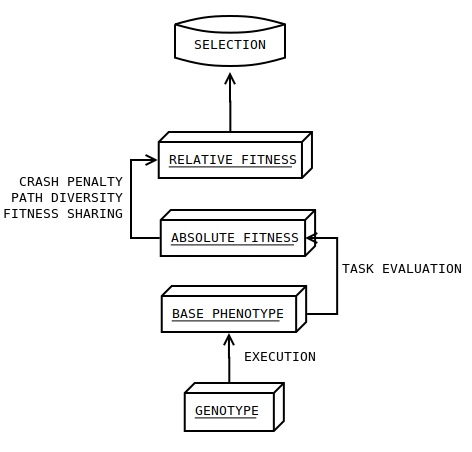
\includegraphics[width=.9\linewidth]{../images/evaluation_model.png}
\caption{\label{fig:orga003938}
High-level overview of the ontogenesis and evaluation process. The ``path diversity'' component will not be introduced until we reach \S \ref{org204263f}.}
\end{figure}

The algorithms explained above all depend, either directly or in the way they
hang together, on having a way to evaluate the ``fitness'' of arbitrary genotypes.

The genetic programming literature often enlists the biological distinction
between \emph{genotype} and \emph{phenotype}.

\subsection{From Genotype to Phenotype}
\label{sec:org9e7583f}
\label{org52d2781}

``Genotype'' is used to refer to the immediate representations of the individuals
in the population, as sequences of semantically uninterpreted instructions. It
is, in a sense, a purely \emph{syntactic} concept. The genotype is the genetic syntax
of an individual in the population, and belongs to the domain of the genetic
operators -- crossover, mutation, and so on, all of which operate on syntax alone,
at least in principle.\footnote{It could be argued that the fragility mechanism described above leaks some
  amount of semantic/phenotypic information into our genetic operations, but
  this is no cause for concern -- the distinction is simply descriptive, and
  carries no prescriptive force.}

\emph{Selection}, however, does not directly operate on genotypes but \emph{phenotypes}.
In the context of genetic programming, ``phenotype'' is the name given to the semantic
interpretation of an individual's genetic code. If the genotype is a sequence of
instructions, then the phenotype is the behaviour expressed when that sequence is
\emph{executed}. 

One could argue \footnote{And, if memory servers, this \emph{has} been argued\ldots{} but memory seems unable to serve either source or citation.}  that the notion
of phenotype should be constrained further still, to refer not just to the semantic
interpretation of the genome, but to \emph{the result of applying the fitness function
to that interpretation}. 
While this distinction does bring some clarity to the issue, and give the engineer
a better view of \emph{what}, exactly, is the subject of selection, it does deprive us
of a nice term for the \emph{intermediate representation}, between genotype and fitness
value. In \gls{roper}, in particular, the semantic image of the genotype is complex
enough that it's worth distinguishing from its later collapse into a fitness value,
for some purposes. We have, moreover, set things up in such a way that it is possible
to vary the \emph{fitness function} while keeping the semantic image -- what we call the
phenotype -- constant. It is simpler, in this case, to ``carve nature at the joints'',
and define the fitness function as a function \emph{from phenotypes to floats}, rather
than as much more complex function from genotypes to floats. The floats, in this
case, will be called ``fitness values'', rather than phenotypes, as Bahnzaf would have it.

As for the function from genotypes to phenotypes -- the semantic evaluation function
-- we might as well keep on pilfering biology textbooks for our terminology, and
refer to it as \emph{ontogenesis}.

\subsection{Ontogenesis of a ROP-chain}
\label{sec:org454c5a7}

Our definition of ontogenesis in \gls{roper} should be no suprise: it is simply the
execution of the ROP-chain payload encoded in the genotype in the ``womb'' 
of the host process. 

If we strip away the clump structure, and associated metadata, such as fragility
ratings, with which we saddled our genotypes in order to provide better traction
to our genetic operators, what remains is just a stack of fixed-width integers.
Some of these integers index ``gadgets'' in the host process, while others are
there only to provide raw numeric material to register and memory operations. If
we take this stack, pack it down to an array of bytes, and write it to the stack
memory of the host process, we should be able to evaluate it simply by popping
the first item on the stack into the instruction pointer -- which is precisely
what would happen when a \texttt{pop \{ip\}} return instruction is executed.

From that point on, we only need to sit back at watch as the ensuing cascade of
returns executes our payload. This is no different from what takes place in
a ROP-chain attack in the wild -- aside from a few simplifications: for the time
being, we are abstracting away from any particular attack vector or preexisting
machine state. The registers of the virtual machine are all initialized to arbitrary,
constant values, and we don't bother to ask \emph{how} the ROP payload happened to get
written to the stack. The stack is of fixed size, and restricted to the region
of memory that the ELF program headers precribe for it -- thereby placing an upper
bound on the effective size of individuals in our population -- but the exact
address of the stack pointer at the moment of inception is not based on any
observed process state, just set, conveniently, to the centre of the available
stack segment. No consideration, as of yet, has been given to avoiding ``bad
characters'' in our payloads, though introducing this restriction would be fairly
trivial. Execution is terminated as soon as any of the following conditions obtain:
\begin{enumerate}
\item the value of the instruction pointer is 0;
\item the \gls{cpu} has thrown an exception (a segmentation fault, a bad instruction,
division by zero, etc.);
\item some fixed number \(n\) of instructions has been executed.
\end{enumerate}

The first outcome is treated as a ``well-behaved'' termination, as though the
payload had reached its proper conclusion. Null bytes are written to the
stack just beneath each payload, with the intention of having \texttt{0x00000000}
popped into the instruction pointer by the final return statement. This condition, 
of course, can easily be gamed by an individual that finds another means of
zeroing out its instruction pointer, with something like
\begin{verbatim}
xor r3, r3, r3
mov ip, r3
\end{verbatim}
for example. 

The second and, to a lesser extent, the third outcome both result in a variable
penalty to fitness, the details of which will be discussed in \S \ref{org5272f96}.

The execution of the ROP chain payload is, in the context of \gls{roper}, our
ontogenesis function: it gives us the phenotype, the behavioural, semantic
profile of the genotype. It is to this structure that the fitness functions
are applied. 

\subsection{Fitness Functions}
\label{sec:orgdb1bd75}
\label{org5272f96}

Each of the fitness functions with which we've experimented begin with a partial
sampling of the individual's behavioural profile, generally restricted to just
a few features:
\begin{enumerate}
\item the state of the \gls{cpu}'s registers at the end of the individual's execution;
\item the number of gadgets executed, as determined by the number of \texttt{return}
instructions evaluated;
\item whether or not a \gls{cpu} exception has been thrown.
\end{enumerate}

This behavioural synopsis is then passed to a task-specific fitness function. We
experimented with three types of task : 
  a. reproduction of an specific register state, such as we might try to achieve
     in order to prepare the \gls{cpu} for a specific system call, for example;
  b. classification of a simple data set, using supervised learning techniques;
  c. participation in an interactive game, where the evaluation of the payload
     makes up the body of the game's main loop.

The task-specific function maps the behavioural synopsis onto a double-width float,
between 1.0 and 0.0, with better performance corresponding to lower values. 
The exact nature of the tasks and performance of the system will be discussed in
detail in Chapter \ref{org8167c36}. For the time being, the matter of \gls{cpu}
exceptions deserves closer comment.

\subsubsection{Failure modes and crash rates}
\label{sec:orgce57c49}

Our population of random ROP-chains begins its life as an extraordinarily noisy
and error-prone species. The old problem of \emph{computational brittleness}  resurfaces here in full force: the odds of a
randomly generated chain of gadgets executing without crashing is extremely
small  -- under 5\%, on average, at the
beginning of a run.  If we were to let each crash count as unconditionally
lethal, this would impose such a tremendous selective pressure on the population
as to make it virtually unevolvable. What few islands of stability exist in the
initial population would be cut off form one another by an inhospitable ocean of
segfaults, leaving little room for exploration.

Fortunately, our chains have the luxury of being raised in the safety of a
virtual nursery, and nothing obliges us to make crashes unconditionally fatal.
We have at least two alternative possibilities:

\begin{enumerate}
\item apply a fixed penalty to fitness in the event of a crash,
\item make the crash penalty proportionate to the ratio of
the chain that executed prior to the exception, measured in gadgets
\end{enumerate}

\Gls{roper} takes the second approach, and implements it by
trapping the return instructions in the Unicorn emulator. This lets us smooth an
abrupt cliff in the fitness landscape down to a gentle slope, incentivizing
adaptations that minimize the likelihood of crashing while at the same time
leaving room to reward specimens that do a good job of solving the
problems posed to them, even if they botch the landing. This prevents us from
sacrificing a number of useful genes, and gives them a chance to decouple from
their pathological counterparts, through crossover, or to be repaired through
mutation.

With this modification to the fitness function in place, the percentage of
chains that crash before completing execution has a tendency to drop to less
than 10\% within a few hundred generations.  What's
particularly interesting is what happens when the average fitness of the
population hits a plateau: the crash rate begins to rise again, until the
plateau breaks, and the error rates begin to drop again. A plausible explanation
for this behaviour is that we are seeing the genetic search start to explore
riskier behaviours as the competition between combatants in each tournament
slackens. As soon as a new
breakthrough is discovered in the problem space, the competition once again
hardens, and crash-prone behaviour becomes a more severe liability. In this way,
he fitness landscape, as a whole, becomes elastic.

\subsection{Fitness Sharing}
\label{sec:org2e2d7b5}
\label{org48435b5}

The most serious problem that \gls{roper}'s populations appear to encounter, particularly
when dealing with relatively complex problem spaces -- classification problems or
interactive games -- is the depletion of diversity. 

As a population becomes increasingly homogenous, the exploratory potential of the
genetic operations becomes more and more constricted. There are two distinct, but
closely related, forms under which diversity should be considered here: genotypic
diversity and phenotypic diversity. At the beginning of the evolutionary process,
when the population consists entirely of randomly-initialized specimens,
genotypic diversity is likely at its historic peak: the sum of genetic
differences between each specimen and every other is maximal, with no
discernible ``family resemblance'' between them, beyond those afforded by chance.
Behavioural, or phenotypic, diversity, however, is typically rather meager at this
point. Unless the problem is extremely simple, and likely to be solved by random
search, the odds are that almost every specimen behaves in an effectively similar
fashion: near-total failure. Nevertheless, if sufficient genetic material exists, however, and if
the fitness function is sufficiently subtle, \emph{some} phenotypic gradients will 
distinguish themselves from the white noise of failure, and it is these minor differences
that selection will accentuate. As a result, the population will often experience a
``Cambrian Explosion'' of some form in the early phases of the evolutionary process: a
tremendous flowering of phenotypic diversity, paid for by a reduction in genotypic
diversity (at least insofar as we can measure genotypic diversity in terms of raw
hamming distances or bitstring similarity, without giving any consideration to structure).
The danger is that some particular family of phenotypes will be so strongly favoured
by selection that its corresponding genotypes \emph{consistently} replicate faster than any
others, squeezing their rivals out of the population altogether. This can lead us to a
point where the exploratory power of recombination is nearly exhausted: the only remaining
sources of novelty, now, is the slow trickle of random mutation or the creation of new,
random individuals \emph{ex nihilo}. The likelihood of this situation being disrupted by
sheer randomness, however, is as small as that of discovering competitive solutions to
the problem set through random search. The result is that evolution stagnates, if not
eternally, at least for much longer than we, as experimenters and engineers, would care
to wait.

When the problem set we are dealing with is plural -- as it is in the second and third types
of fitness function, listed in \S \ref{org5272f96} -- one way that diversity depletion often
occurs is through \emph{hypertelia}, or an adaptive fixation on low-hanging fruit.\footnote{The notion of hypertelia used here has been borrowed from Gilbert Simondon. See,
  for example, the discussion in Chapter II, Section I, of 
  \emph{On the Mode of Existence of Technical Objects}, which begins, ``The evolution of technical objects manifests certain hypertelic phenomena which
  endow each technical object with specialization, which causes it to adapt badly
  to changes, however slight, in the conditions of its operation or manufacture.''} 
It is common for some subset of the problem set to be considerably simpler than the rest,
or for distinctions between certain classes in a classification problem to be more computationally
tractable than distinctions between other, more ambiguous or complexly defined classes. 
It is consequently likely that the population will produce specimens that are capable of
handling those simpler problems and clearer distinctions before anything exhibits comparable
skill in handling the ``harder'' problems. So long as the fitness function remains static,
selection will magnify this discrepancy, and the simple-problem-solvers will enjoy a persistent
reproductive advantage over any specimens that may be still fumbling their way through the
more complex regions of the fitness landscape. Once the bottomfeeders reach such numerical
dominance that they start to appear in the majority of tournaments, there remains very little
selective advantage in tackling any other aspect of the problem space, and the population
suffers a rapid loss of phenotypic diversity. Whatever tacit grasp on the problem
space's more challenging terrain may have emerged in the population up to that point is
quickly eclipsed and snuffed out. In the evolutionary computation literature, this dynamic
is referred to as ``premature convergence''. 

What guards natural ecosystems against this development are the merciless
pressures of crowding, scarcity, competition, which introduce a dynamic selective
pressure for phenotypic diversity. The fitness rewards provided by low-hanging
fruit are no longer boundless, but diminish in proportion to the number of
individuals that reap them. At a certain point, the selective advantage no longer
lies with those individuals that exploit the same, simple regions of the problem
space, but with those who discover a niche that hasn't yet been picked thin by
crowds of competitors.

A similar tactic can be adopted in evolutionary computation, where it goes by
the name of ``fitness sharing''. At least two implementations of this strategy
have become canonical in the literature: \emph{explicit} fitness sharing, introduced
in \cite{deb89}, and \emph{implicit} fitness sharing, introduced in \cite{smith92}.

The underlying idea in both is that \emph{selective advantage should be diluted by
nondiversity}. Explicit fitness sharing ``relies on a distance metric to cluster
population members,'' writes R.I. McKay in \cite{mckay00}. ``Implicit fitness sharing,''
by contrast, ``differs from the explicit form in that no explicit distance metric
is required. Instead, all population members which correctly predict a particular
input/output pair share the payoff for that pair.'' 
In \gls{roper} we adopt a variation on the latter approach. The implementation is as
follows:

\begin{enumerate}
\item each problem is initialized with a baseline
\texttt{difficulty} score. It doesn't much matter which value is used for this,
but setting it to the inverse of the probability of solving the problem 
by random guess works well, when dealing with classification problems;

\item each problem is also allocated a \texttt{predifficulty} vector, which begins empty.
Every time an individual responds to the problem, its (its fitness assessment
for that particular problem) score is pushed into its \texttt{predifficulty} vector.

\item after a one ``season'' of tournaments has elapsed -- where the length \(N\) 
of a season is defined as
$$N \gets \frac{\texttt{population\_size}}{\texttt{tournament\_size} * (1 - x)}$$
where \(x\) is the probability of ``headless chicken crossover'' (cf. Algorithm
\ref{alg:headless}), we iterate through the problem set. 
Each problem \(e\)'s \texttt{difficulty} field is set to the mean of the predifficulty
vector. More difficult problems, at this point, are associated with a higher
difficulty score, which is always a float between 0.0 and 1.0.

\item once difficulty scores are available for each problem, the relative fitness of
each individual responding to it can be assessed: it is just the base, or ``absolute'',
fitness score, multiplied by the inverse of the difficulty. If, for instance, 
\(X\) receives 0.75 on a problem for which the average performance has been
0.1, then \(X\)'s relative fitness is \(0.75 * (1.0 - 0.1) = 0.75 * 0.90 = 0.675\).
If, on the other hand, it receives 0.2 on a problem for which the average performance
is a miserable 0.98, then its relative fitness comes to 0.004, reflecting the
rarity of its talents.
\end{enumerate}

\subsubsection{Mechanisms of Selection}
\label{sec:org56d9222}
This brings us back to where our algorithmic overview began: to the tournament
algorithm used to select mating pairs. In the interest of bolstering the diversity
of the population, and staving off premature convergence, we incorporated two
fairly well-known modifications into the steady-state, tournament selection
scheme described in Algorithm \ref{alg:evolve}: the partitioning of the population
into ``islands'' or ``demes'', with rarefied points of contact, and the occasional use of 
``headless chicken crossover'' as ongoing supply of novelty to the gene pool.

\paragraph{Islands}
\label{sec:org77555e3}
The mechanism used to isolate \gls{roper}'s subpopulation or ``demes'' is extremely simple:
when we go to select our candidates for each tournament, we do so by choosing 
\(n\) random indices \(\vec{i}\) into the general population array, but each time we
choose, we restrict ourselves to choosing integer between 0 and some constant, 
\(\text{island\_size}\), decided in advance. The index \(j\) of the candidate is then
set to \(j \gets i * \text{island\_size} + \text{island\_id}\). So long as this 
restriction is in place, each individual will only directly compete with its
compatriots, throttling the speed at which the population is likely to converge
on a single dominant genetic strain. This throttle is modulated by allowing the
selection of every \(m^{th}\) candidate to be chosen from the general population,
without any regard given to island of origin. The migration rate, \(m\), can be
easily adjusted to experiment with more and less genealogically interconnected
populations.

\paragraph{Headless Chicken Crossover}
\label{sec:orgb6b403c}
As a means of supplying the gene pool with an additional spring of novelty,
we also make use of a simple technique called ``headless chicken crossover'',
which amounts to a small patch to Algorithm \ref{alg:evolve}: we replace
line \ref{alg:evolve:line:candidates} with Algorithm \ref{alg:headless}.

\begin{algorithm}
\caption{Headless Chicken Patch}
\label{alg:headless}
\begin{algorithmic}[1]
\REQUIRE {$H$: float, with $0.0 < H < 1.0$}
\REQUIRE {$\mathbf{G}, \mathbf{P}, \text{min}, \text{max}$: the parameters needed for
Algorithm \ref{alg:spawn}: the gadget pool, the integer pool, and the minimum and maximum
length of new individuals}
\STATE {$\frak{R}, i \gets \frak{R}$, {pick a random float} $0 < i < 1$}
\IF {$i < \textrm{headless\_chicken\_rate}$}
\STATE {$\frak{R}, \textrm{candidates} \gets$ using $\frak{R}$, pick $n-1$ from $\Pi$}
\STATE {$\frak{R}, \textrm{candidates} \gets \textrm{candidates} \cup \textit{spawn}(\frak{R},
\mathbf{G}, \mathbf{P}, \texttt{min}, \texttt{max})$}
\COMMENT {Using Algorithm \ref{alg:spawn}}
\ELSE
\STATE {$\frak{R}$, candidates $\gets$ using $\frak{R}$, pick $n$ from $\Pi$}
\COMMENT {As before}
\ENDIF
\end{algorithmic}
\end{algorithm}


\section{Remarks on Implementation}
\label{sec:org35d3f11}

The system described above has been implemented using the Rust programming
language, and the Unicorn emulation engine \cite{unicorn} \cite{nguyen15}. 

Rust was chosen for its speed, type-safety, and functional niceties, 
though this decision wasn't entirely unarbitrary -- prototypes of the
system in Lisp, Haskell, and OCaml are still strewn about my hard drives
and Git repositories in various states of incompleteness. The decision
to make use of the Unicorn framework remained somewhat more constant.
Evaluating arbitrary \gls{rop} chains on bare metal turned out to be
every bit as hazardous and messy as it sounds, and so the need to find
a suitable virtualization framework became apparent very early in the
project. Spinning up full-fledged \gls{qemu} \glspl{vm} for each evaluation
-- or even for each evaluation that ended in a fatal system state --
would bring with it a prohibitive amount of overhead. I needed something
that would let me evaluate thousands upon thousands of individuals within
a reasonable timeframe. 

Unicorn, which its authors describe as, ``a lightweight multi-platform,
multi-architecture \gls{cpu} emulator framework'', exposes the \gls{cpu}
emulation logic of \gls{qemu}, while abstracting away from \gls{io} devices and any
interface with the operating system, along with all their associated overhead.
The machine state of the emulator remains transparent, and is easily
instrumented by the user. This makes Unicorn ideal for performing a fine-grained
semantic evaluation of \gls{rop} chains, under the assumption of a given \gls{cpu}
context. The evaluation, that is to say, is strictly ``concrete'' -- it will tell
us only how a given chain will behave, \emph{assuming that the \gls{cpu} context and
memory space is in such and such a state}. This can be seen as an limitation of
\gls{roper}, as compared to procedurally deterministic but symbolically
indeterministic \gls{rop} compilers like \emph{Q} \cite{schwartz11}, which makes use of symbolic
execution (via \gls{bap}) to precisely determine the semantic valence of each
available gadget so as to \emph{explicitly} fashion them into the \gls{isa} targetted
by \emph{Q}'s own compiler. What \gls{roper}'s procedurally stochastic and
semantically concrete (i.e. ``deterministic'') approach loses in semantic
precision and robustness, however, is made up for with a singular cunning when
it comes to exploiting the \emph{particular}, concrete state of its host process. Its
task, after all, is not to craft a portable, reusable \gls{rop} payload that can
be cut-and-pasted, off-the-shelf into arbitrary attack contexts, but to craft
payloads that are as idiosyncratically adapted to the peculiarities of its
chosen target as a moth to its orchid.

\subsection{Initialization of the environment}
\label{sec:orgaec825a}
In the discussion of the algorithmic specification of \gls{roper}, above,
we have, for the most part, abstracted away from the environment in which
the evolutionary process occurs. Setting up this environment is the first
task of the engine, and it proceeds as follows.

It begins by parsing and analysing the target binary -- either a standalone
executable, or a shared library file. \footnote{Or, in principle, any region of
executable memory. I am planning to have ROPER handle core dumps, for instance}   \Gls{roper} is currently 
only prepared to handle \gls{elf} binaries targetting 32-bit, little-endian
\gls{arm} architectures, and though there's no \emph{essential} reason for any of these
restrictions, and the system could be fairly easily adapted to handle other
\gls{abi} formats (such as Apple's \gls{macho} or Window's \gls{pe} formats), or
other architectures (some tenative work on adapting \gls{roper} to \gls{mips}
is already underway, and it turns out to be fairly straightforward to 
take on other \gls{risc} \glspl{isa}; \gls{cisc} \glspl{isa} pose a few more
challenges, but tend to make for extremely fertile gadget sets -- the
\gls{x86} instruction set is so vast and intricate, for example, that
it can be a challenge to find a string of bytes that \emph{can't} be parsed
as a series of \gls{x86} machine instructions!). 

\Gls{roper} reads the \gls{elf} program headers and loads the program data into the
memory of a cluster of Unicorn emulator instances, at the appropriate addresses,
and with the appropriate permissions, just as the Linux kernel would do when
launching the executable on the metal. While doing this, \gls{roper} (optionally)
can ensure that \gls{w+x} is enforced, even if not strictly required by the
binary. (In all of the experiments documented in Chapter \ref{org8167c36},
\gls{w+x} \emph{has} been enforced.)

Since \gls{roper}, like any genetic programming system, relies heavily on
randomness, a word or two about its \gls{PRNG} is in order. The \gls{prng}
used is supplied by Rust's default \texttt{std::rand::thread\_rng} function, which,
as of version 0.5 of the \texttt{rand} library, rests on an implementation of
the cryptographically secure \gls{hc-128} algorithm \cite{wu08}, seeded on a per-thread
basis by the operating system's entropy pool. In the current implementation,
the seeds passed to this generator are not logged, and cannot be manually specified
by the user, which makes the exact replication of a run impossible. I hope to
address this shortcoming in a future overhaul of the codebase. The salient point
about the \gls{prng}, for now, is that it is of fairly high quality, and \emph{should}
not be vulnerable to being exploited by the populations. 





\begin{savequote}
\textsc{Dr. Ian Malcolm} John, the kind of control you're attempting simply is... it's not possible. If there is one thing the history of evolution has taught us it's that life will not be contained. Life breaks free, it expands to new territories and crashes through barriers, painfully, maybe even dangerously, but, uh... well, there it is.

\textsc{John Hammond} [sardonically] There it is.

\textsc{Henry Wu} You're implying that a group composed entirely of female animals will... breed?

\textsc{Dr. Ian Malcolm} No. I'm, I'm simply saying that life, uh... finds a way. 
\qauthor{Michael Crichton, \emph{Jurassic Park}}
\end{savequote}

\chapter{Experimental Studies}
\label{sec:orgdb92958}
\label{org8167c36}

\begin{figure}[htbp]
\centering
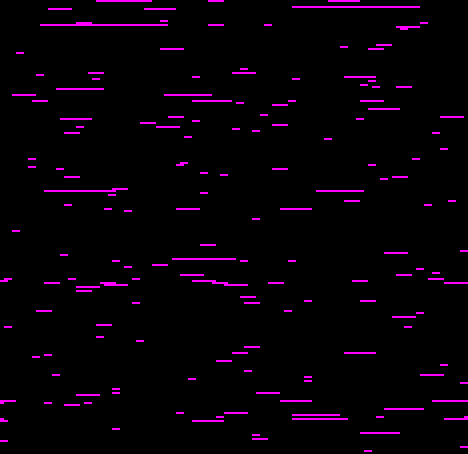
\includegraphics[width=.9\linewidth]{../images/tomato-RT-N18U-httpd_heatmap.png}
\caption{\label{fig:orga2f0b1d}
Bitmap representation of the gadget distribution in the tomato-RT-N18U-httpd \gls{elf} binary}
\end{figure}

\section{Overview}
\label{sec:org1605fcf}
\label{orge9e076e}

As of the time of writing, I have experimented with four distinct classes of
fitness functions in \gls{roper}, with a handful of variations within each class.
Though \gls{roper} has been tested with numerous executable \gls{elf} binaries,
compiled for the 32-bit \gls{arm} architecture, for the sake of consistency, 
unless otherwise noted, all of the experiments discussed here make use of
a web server binary blob, pulled from the \texttt{tomato-RT-N18U} router firmware
image \cite{tomato-RT-N18U}. The distribution of gadgets harvested from this
binary's \texttt{.text} section are plotted in figure \ref{fig:orga2f0b1d}, to which
I will make frequent reference in the subsequent heatmap overlay images.

In the following subsections (\ref{org127143f}, \ref{org86f0f05},
\ref{orgce1b46b}, and \ref{orgece58eb}), I will outline each task set that
\gls{roper} was given to perform, and specify the way in which each was
incorporated into \gls{roper}'s fitness function.

In \S \ref{org1f9fea0}, I will walk through some of the more interesting results
gleaned from each experiment, and in \S \ref{orgd92d702}, I will lay out certain
conjectures that address an enigma in the observed results, and set out another
series of experiments to test it. 

\subsection{The null task}
\label{sec:org890f2f5}
\label{org127143f}

As discussed in \S\S \ref{org0b80a57} and \ref{orgdda015b}, when designing a genetic
system, a question that naturally arises as to what constraints are brought into
play by the shape of the system itself, in its genotypic and phenotypic topography,
independent of any particular fitness function that could be applied to it. In the
case of simple and unilateral genetic algorithm systems -- where there is no distinction
between phenotype and genotype (the genetic syntax of individuals and their 
operational semantics), it is possible for the system to be strongly \emph{ergodic}.
Under less harmonious conditions, however, there may exist various attractors in
the genotypic and phenotypic landscapes, and in their interaction, that incline
the system to converge in ways that are relatively independent of any specific
fitness function. 

One way to empirically study these dynamics is to define an
effectively uninformative fitness function, one that metes out rewards arbitrarily
and inscrutably, without any detectable pattern. A cryptographically secure
random number generator is well suited to this particular sort of absurdity, and
this is how \gls{roper} implements its null task.\footnote{In the current implementation, this task can be chosen by setting the 
  problem type to \texttt{kafka}, in the configuration.} 

And since, in each of the other experiments, I enforce some form of crash penalty
as a component of the fitness function (see \S \ref{org5272f96} for details),
it would make sense to study what effects this pressure alone, abstracted from
the others, has on the population dynamics. For this reason, I will introduce
a second series of null task runs, in which the only non-random variable used
in reproductive selection will be the crash penalty. 

\subsection{Preparing the parameters for a system call}
\label{sec:orge95a280}
\label{org86f0f05}

This task is the most immediately practical of the set, and comes the closest to
a practical, ``real world'' application of \gls{roper} in the domain of application
security. One of the most common use cases for a \gls{rop} chain is to prepare
the \gls{cpu} context for a particular system call, permitting the attacker to
read or write to a file, open a socket, execute a program, or any other task
that requires the cooperation of the operating system. To do this in assembly
or machine code, the programmer needs to set certain registers to contain and
point to the relevant values. To call \texttt{execv("/bin/sh", ["/bin/sh"], NULL)}, 
for instance, and spawn a shell process, on the \gls{arm} architecture, she needs
to set register \texttt{R0} to point to the null-terminated string \texttt{"/bin/sh\textbackslash{}0"}, 
register \texttt{R1} to point to a pointer to that string, set \texttt{R2} to zero, and
set \texttt{R7} to the code for this particular system call. Once this is done, dispatching
the call is just a matter of executing the \texttt{SVC} instruction. To perform this
operation with a \gls{rop} chain, the same requirements must be met, but in a more
roundabout fashion, since the \gls{rop} hacker isn't able to execute any instructions
directly, but must conduct the processor to execute a series of gadgets whose
cumulative effect is to prepare just this machine state. The final gadget in the
chain, however, is trivial: it is just the address of an \texttt{SVC} instruction, followed,
perhaps, by whatever series of gadgets is necessary to clean up the process and 
restore the normal flow of execution, if stealth is desired. (Though it's entirely
possible, in most cases, to simply let the host process crash after performing the
desired call -- it's just a bit sloppier, and can bring about other problems in the
context of a real-world attack.)

The task we assign \gls{roper} is to carry out the preparation stage of this operation,
but it can easily be extended to complete the call -- it is, after all, just a matter
of appending a single, trivial gadget to the chain, which can almost always be found
in binary, since the \texttt{SVC} call is perfectly generic and does not embed any of its
arguments in the instruction itself. This step is omitted in our experiments only
because Unicorn abstracts away from any interaction with the operating system, and
doesn't handle system calls in a meaningful way. The cleanup stage is more context-sensitive
and complex, but something I may experiment with in the future, in order to prepare
fully deployable payloads with \gls{roper}.

The fitness function defined for this task aims to be a gauge of the distance between
the register and memory state resulting from an individual chain's execution, and
the state required for the call. ``Distance'', here, however, is a tricky concept, and
it isn't at all obvious how it should be defined in such as way as to both track
material progress towards the goal in view, and remain efficiently calculable. Ideally,
it would be defined as edit distance in the Markov chain that represents a genotype's
trajectory through probability space: how many generations, or applications of the
genetic operators, are required to achieve the target state, and how probable are each
of those genetic pathways? In practice, we make do with a very loose approximation of
this ideal:

\begin{itemize}
\item For each target immediate value, we first check the execution result in the target register,
and take the hamming distance between the two values (the number of 1s in 
\(\text{target} \oplus \text{result}\)), and divide it by the maximum hamming distance
(32, on this architecture), storing the quotient in the variable \texttt{nearest};
\item If \(\texttt{nearest} \neq 0\), we iterate through the remaining result registers,
and calculate the hamming quotient with the target for each value found there. We
then apply a ``wrong register'' penalty to the quotient, and if the result is still
less than \texttt{nearest}, we rebind \texttt{nearest} to the result.
\item We then pass to our memory samples from the execution -- one for each register that
could be validly referenced in the machine state at the end of execution, each holding
\(n\) bytes (currently, \(n\) is set to 512, but this may undergo tuning) from the
engine's memory, starting with the address in the register. We scan the memory
sample for the desired value, and, if found, we return the quotient of the value's
offset by the length of the sample (e.g., if we find it at offset 256, then we
return \(\frac{256}{512} = 0.5\)). If the index of the register dereferenced to
that memory sample is the same as the target's, then we consider this quotient
as a new candidate for \texttt{nearest}, after applying a ``right value, but needs to be
dereferenced'' penalty. If there is a mismatch in the register index, we also 
apply the ``wrong register'' penalty, and do the same.
\item After completing these iterations for a particular target register, 
we push the final setting of \texttt{nearest} into an error vector, to be considered later.
\item \texttt{nearest} is then reset to the maximum value of \(1.0\), and we repeat the process for
the next immediate target register.

\item We then move on to the indirect targets in our target vector, and repeat more or
less the same process, first scanning the memory samples returned from the
individual's execution in the emulator, recording any findings, and then passing
on to consider the immediate values in the register, where we calculate the hamming
quotients, applying the same penalties as above wherever there occur mismatches 
between target and resultant register index, or mismatches between desired indirection
and resultant immediacy. At the end of each check, the final value of \texttt{nearest} is
pushed to the error vector.
\item Finally, we take the mean of the values in the error vector, and return it as a float
between \(0.0\) and \(1.0\): this is the fitness value for that particular evaluation.
\end{itemize}

The function used for the ``wrong register'' and ``needs to be dereferenced or indirected''
penalties was, like most details in \gls{roper}, arrived at through a great deal of
trial and error, and at the time of writing has settled into \(1 \sqcap \sqrt{x+0.1}\),
which seems to generate a reasonable amount of pressure while still maintaining
a traversable gradient in the fitness space. Restricting the primary distance measure
to hamming distance and forward linear scans feels like a fairly crude approximation,
but seem serviceable enough for now.

This is quite a bit to keep in mind at once, and so a visual simplification
might help the reader form an intuition of how this function works: if we
imagine the state of the CPU after execution as a point \(p\) in
(\(|\text{registers}|*2\))-dimensional space -- using an immediate and an indirect
dimension for each register, using different metrics -- then the target pattern
is just an \(n<16\) dimensional hypersurface \(S\) in that space, and the fitness
function is simply the distance from \(p\) to \(S\), given a suitable metric, and
scaled to a float between 0.0 and 1.0.

\subsection{Classification problems}
\label{sec:orgc3fe6f7}
\label{orgce1b46b}

\Gls{roper}'s pattern-matching capabilities allow it to automate tasks commonly
undertaken by human hackers. The end result may not \emph{resemble} a ROP-chain
assembled by human hands (or even by a deterministic compiler), but its function
is essentially the same as the ones carried out by most human-crafted
ROP-chains: to prepare the \gls{cpu} context for this or that system call, so that
we can spawn a shell, open a socket, write to a file, dump a region of memory,
etc.

In this series of experiments, we'll see that \gls{roper} is also capable of
evolving chains that are, in both form and function, entirely unlike anything
designed by a human. Though it is still in its early stages, and its
achievements so far should be framed only as proofs of concept, \gls{roper} has
already shown that it can evolve chains that exhibit learned or adaptive
behaviour. To illustrate this, we will set \gls{roper} the task of classifying, first,
a toy data set, designed for simplicity, and, second, Ronald Fisher and Edgar
Anderson's famous \emph{Iris} data set.

The Iris data set is a well-worn benchmark for training elementary
machine learning systems,\footnote{``This is perhaps the best known database to be found in the pattern
  recognition literature,'' reads the data set information note at \cite{iris}.} and to the machine learning specialist, there is
nothing particularly interesting about yet another classifier churning out
results for such a relatively unchallenging set.
But, with these experiments, we enter essentially uncharted waters as far as
return-oriented programming -- or even, to the best of my knowledge, any form of
low-level ``weird machine'' exploitation -- is concerned. There is no real
precedent for having anything like a \gls{rop} payload implement even a basic and
rudimentary machine learning benchmark, and so this task is introduced here
entirely as a proof of concept.\footnote{If you're interested in developing an
 intelligent classifier, you're unlikely to consider doing so using the unweildy
 scraps of hijacked process's memory, and if you're interested in crafting a
 low-level attack payload, a reverse shell probably seems like a more sensible
 goal than a moderately clever flower sorter -- unless, of course, what you're
 really after in either field are ways of making machines do strange, strange
 things.} The interest, here, isn't in building a better mousetrap. It's in
showing that one can be built -- or bred -- out of utterly alien materials.


The Iris data set comprises series of four measurements -- sepal length,
sepal width, petal length, and petal width --
for 50 specimens belonging to three different species of iris flower, 150
specimens in all. The task of the classifier is to predict the species when
given the measurements. ``One class is linearly separable from the other 2,''
the documentation on the UCI Machine Learning Repository advises, ``the latter
are NOT linearly separable from each other.'' 
The fitness of each competing \gls{roper} individual, in this context, will
depend on its ability to correctly classify the sample of specimens presented
to it. Since this is a balanced data set, detection rate alone is a sufficient
proxy for accuracy. The four attributes of each specimen will be cast and
normalized as integers, and, for each evaluation case, loaded into four of
the Unicorn \gls{cpu}'s general purpose registers. The candidate chain is then
executed, as described above, and at the end of execution we read the values
contained in three distinct registers, designated as ``output registers'' for
this purpose. Each register represents a ``bid'' for one of the three possible
iris species. The values they contain are cast as signed integers, and the
register containing the largest value is interpreted as a winning bid for
its corresponding species. 

As we will see in a moment, experimentation has shown that an accurate and, if not
altogether efficient, at least timely\footnote{Meaning: you will receive the results before you die.} classification of the set can be achieved by
\gls{roper}, so long as the fitness sharing mechanism discussed in \ref{org48435b5}
is made available to it. 

The base fitness function used in the classification experiments is based on
register-bids: a subset of general purpose machine registers are designated
as ``output registers'', and another, as ``input registers''. At the beginning of
each evaluation case (each exemplar in the training set), the input registers
are loaded with values from the attribute fields. At the end of execution,
data is read from the output registers. Each output register is interpreted
as a signed integer, and taken to represent a bid on a class. The register
with the highest bid decides the individual's ``guess'' at which class the
attributes passed to it represent. In the event of a tie or an incorrect
guess, no points are awarded (the fitness value of this case is set to 1.0,
which is the poorest rating). In the event of a correct guess, 0.0 points
are awarded. That point value is then duplicated into a pair. The first
remains untouched, and is factored into the detection rate or ``absolute
fitness'' of the chain. The second is passed to subsequent modifications.
If the chain threw an exception during execution, for instance, then the
score is raised by a certain factor (which is tunable, and in some experiments,
dynamically variable in response to population trends), but it is constrained
to remain between 1.0 (worst fitness) and 0.0 (best fitness) at every point.
If fitness sharing is in effect, then the modifiable component of the score
has the inverse of the exemplar's difficulty added onto it. (If the chain
scored a 0.0 on an exemplar for which the mean performance is 0.85, for instance,
then it receives an additive boost of 0.15.)



\subsection{``Would you like to play a game?''}
\label{sec:org0f893c1}
\label{orgece58eb}

Naturally, the first question that comes up when you find a way of eliciting
rudimentary, intelligent behaviour from an exploited process is whether it
can play any games. This brings us to our fourth fitness function: we want
to train \gls{roper} to evolve \gls{rop} chains that can play a game of Snake.\footnote{I'm reserving tic-tac-toe for emergencies.} For this purpose, I wrote a simple, machine-friendly implementation of the
classic arcade game in Lisp,\footnote{The code is freely available at \url{https://github.com/oblivia-simplex/snek}.} and set it up to communicate with \gls{roper} over
a TCP connection. \Gls{roper}'s task, here, is to evolve a \gls{rop} chain that,
when run in a loop, can play a more or less competent game of Snake. The \gls{rop}
chain is fed an array of first-person sensor readings, from the snake's perspective,
which indicate the relative distances of objects in the playing field: \emph{apples},
which increase the snake's length, \emph{cacti}, which kill the snake on contact, 
segments of the snake's own body, which are similarly dangerous to collide with,
and the walls of the field, which, again, result in death on contact. 
Points are awarded to the player relative to the number of unique grid coordinates
visited, and the number of apples consumed, before dying. 




\section{A few notes on terminology}
\label{sec:org6205a65}
\label{org0aa24d2}

\subsection{Problems, patterns, and exemplars}
\label{sec:org4aa9972}
\label{org2c1fe05}

\Gls{roper} is designed to handle a variety of tasks, and having a generic term
to refer to the basic units of each task is helpful, in discussing the experiments
that follow. I use ``problem'' for this purpose. 

When the task is a classification task, the ``problems'' may also be referred to as
``exemplars''. When the task deals with preparing a CPU state, I sometimes use the
term ``pattern'' to refer \emph{specifically} to what I \emph{generically} call a ``problem''. 
In interactive tasks, the role of ``problem'' may be filled by a game-space configuration. 

\subsection{Iteration, generation, and season}
\label{sec:org76dfcd3}
\label{org0b70616}

\Gls{roper} employs a steady-state selection model in all of the experiments
discussed in this thesis, and so it's important to distinguish what we mean
by \emph{generation} from what we mean by \emph{iteration}. The notion of ``iteration'',
here, is for the most part external to the actual evolutionary process -- it's 
an artefact of implementation, in a sense, representing only a cycle through
the ``main loop'' of the program, during which one or more tournements are thrown
in parallel. (I say ``artefact of implementation'' with a very large grain of
salt. If there are any fields of study that demand a healthy skepticism towards
what counts as essential to the specification, and what counts as ``mere
implementation details'', they're computer security and evolutionary computation!)
An ``iteration'', in this context, becomes a meaningful evolutionary unit
(modulo abstraction leaks) through a mediating notion that, in \gls{roper},
I've called a ``season'': a season is defined as a sequence of iterations that
is just long enough for it to become highly probable that more or less 
every member of the population has had their shot at a tournement (and, therefore,
a shot at reproduction). In concrete terms, the length of a ``season'' is a
function of tournement size and population size. 

\subsection{Naming scheme for populations}
\label{sec:orga6f6b9e}
\label{org5b4b838}

Mentally keeping track of numerous, varying artificial populations is a challenge at the
best of times, and I've found that assigning short,
pronounceable names to each batch is a useful mnemonic device. For this purpose,
I've borrowed a trick from the designers of \emph{Urbit}, and used strings of six
random letters, following the pattern ``\texttt{consonant vowel consonant consonant vowel consonant}''\footnote{This superficially resembles the namespace that Yarvin and Wolff-Pauly allocate
  to ``stars'' in \emph{Urbit}, but is a bit less constrained: their namespace has room
  for \(2^{16}-1\) names, ours accommodates \((20 * 6 * 20)^2 \approx 2^{11.2}\).}. Using these labels over the course of this chapter lets me avoid circumlocutions
like ``as seen in the second population discussed in \S \$N'', and has the
further advantage of setting up a self-documenting correspondence between the
analyses in this chapter and my system of log files. 


\section{Initial Findings}
\label{sec:orgb70740a}
\label{org1f9fea0}

\subsection{Surveying the landscape with the null task}
\label{sec:org6da1ee2}
\label{org87dcb5a}

Before looking at the behaviour of \gls{roper} under the influence of and constraints
of the semantically nontrivial fitness functions described above, let us first try
to get a sense of how the system behaves \emph{without} receiving any meaningful fitness
information, and then move on to a constraint that is incorporated into each of the
fitness function considers, and acts as their common factor: the one imposed
by the crash penalty.

\subsubsection{Arbitrary selection with no crash penalty}
\label{sec:org48c0934}
\label{orgb694cd1}

\begin{figure}[htbp]
\centering
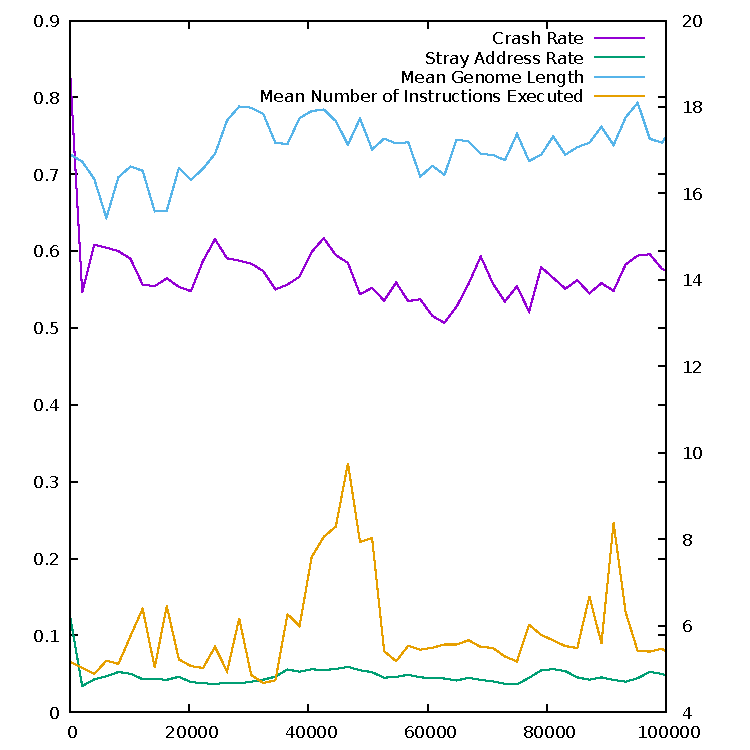
\includegraphics[width=.9\linewidth]{../images/plots/kurlig_kafka_performance.pdf}
\caption{\label{fig:org00ef387}
Performance metrics over \emph{Kurlig} population of 2048, evolving under the absurd fitness function. Crash rate and stray address rate map to left vertical axis, while mean genome length and mean instructions executed map to the right.}
\end{figure}

\begin{figure}[htbp]
\centering
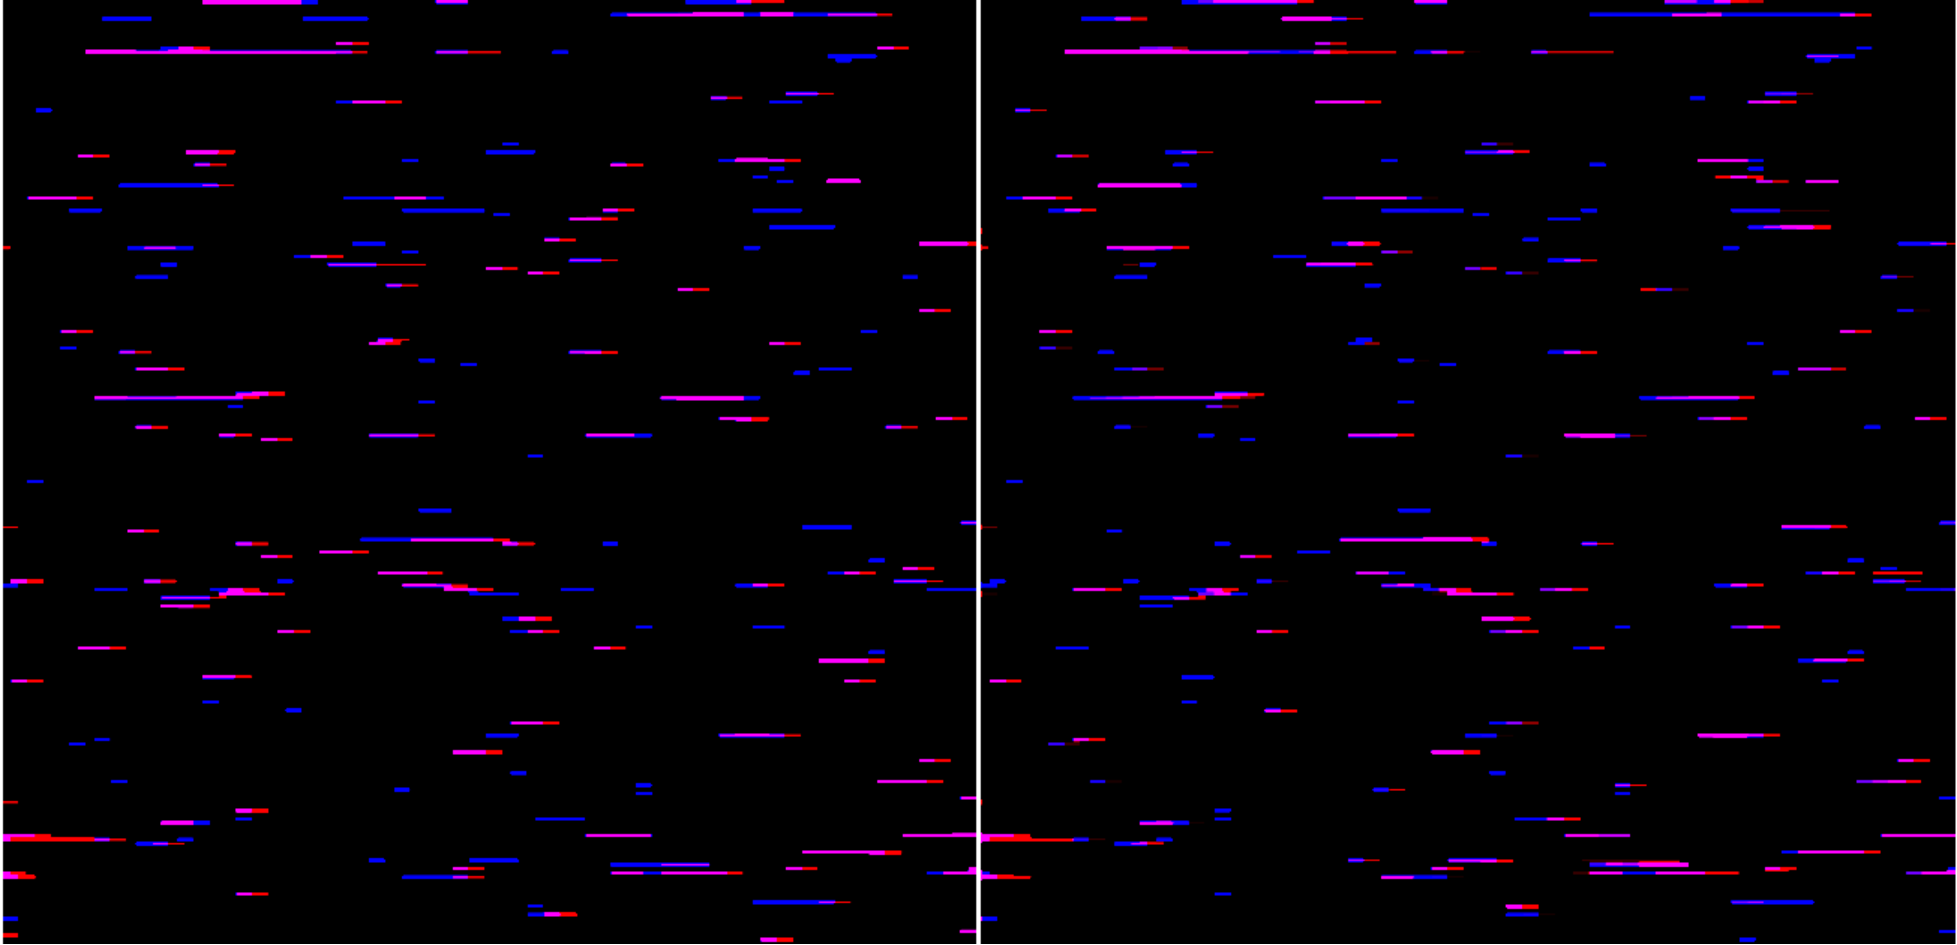
\includegraphics[width=.9\linewidth]{../images/plots/kurlig_heatmap_4_212_montage.pdf}
\caption{\label{fig:orgaaeefc2}
Address visitation heatmap over the tomato-RT-N18U process memory, by the \emph{Kurlig} population, evolving under the absurd fitness function with no crash penalty. Season 4 heatmap displayed on the left, season 212 on the right.}
\end{figure}


The first thing that we wish to learn about how our populations behave under
randomized selection pressure is whether there are any discernible 
trends in the distribution of behaviours in those populations over time. 
One useful view on this distribution is the heatmap of addresses visited over the
course of the run, sampled seasonally. Though not a precise or statistically
significant representation of behaviour, it does, at least, serve to convey a
general impression, at let the eye pick out the more obvious skews in distribution. 

In figure \ref{fig:org8be3697}, we see heatmaps of the the \emph{Xeqcyv} population's
phenotypic distribution sampled at seasons 4 and 212. Qualitatively speaking, the
two maps appear almost identical. There has been no collapse of phenotypic diversity,
and the system even gives the impression of being ergodic.\footnote{See \cite{schmitt01} for a detailed discussion of the conditions under which genetic algorithms exhibit ergodicity.} Acting freely, with
no systematic selective constraints, the mutation operators appear to be successfully
counteracting the pull of genetic drift. 


\subsubsection{Arbitrary selection with crash penalty}
\label{sec:org307b681}
\label{org51cf4aa}

\begin{figure}[htbp]
\centering
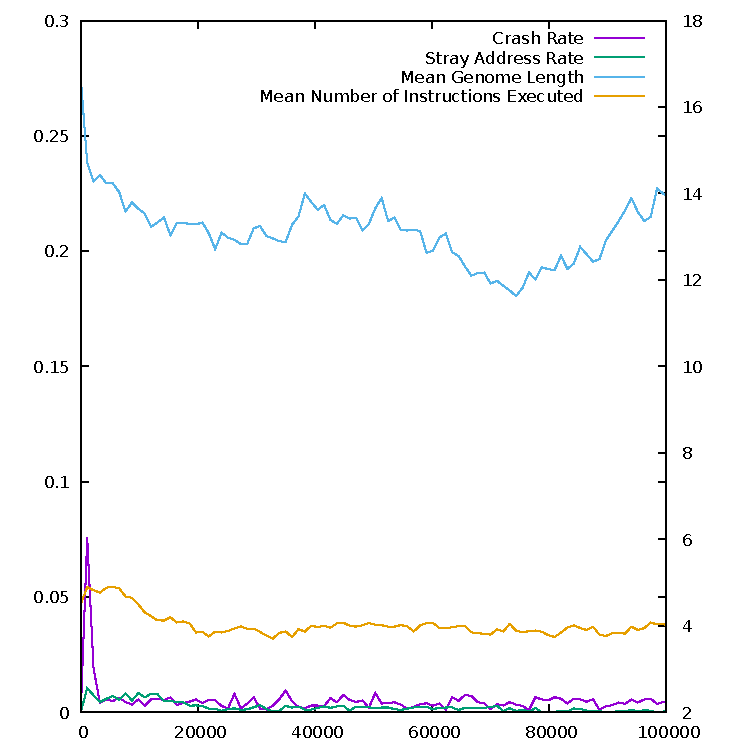
\includegraphics[width=.9\linewidth]{../images/plots/xeqcyv_kafka_performance.pdf}
\caption{\label{fig:org3b7bb3b}
Performance metrics over \emph{Xeqcyv} population, evolving under absurd fitness function with crash penalty. Crash rate and stray address rate map to the left vertical axis, while mean genome length and mean instructions executed map to the right.}
\end{figure}


Surprisingly, even with the crash penalty in place, the distribution of execution
path frequency remained strikingly consistent, at least to a distant and qualitative
inspection. The heatmap snapshots of the population's execution habits at Season 4,
and again at Season 212, showed such little difference that I had to check carefully
to make sure that I had not placed them in the wrong order, in figure
\ref{fig:org8be3697}. 

\begin{figure}[htbp]
\centering
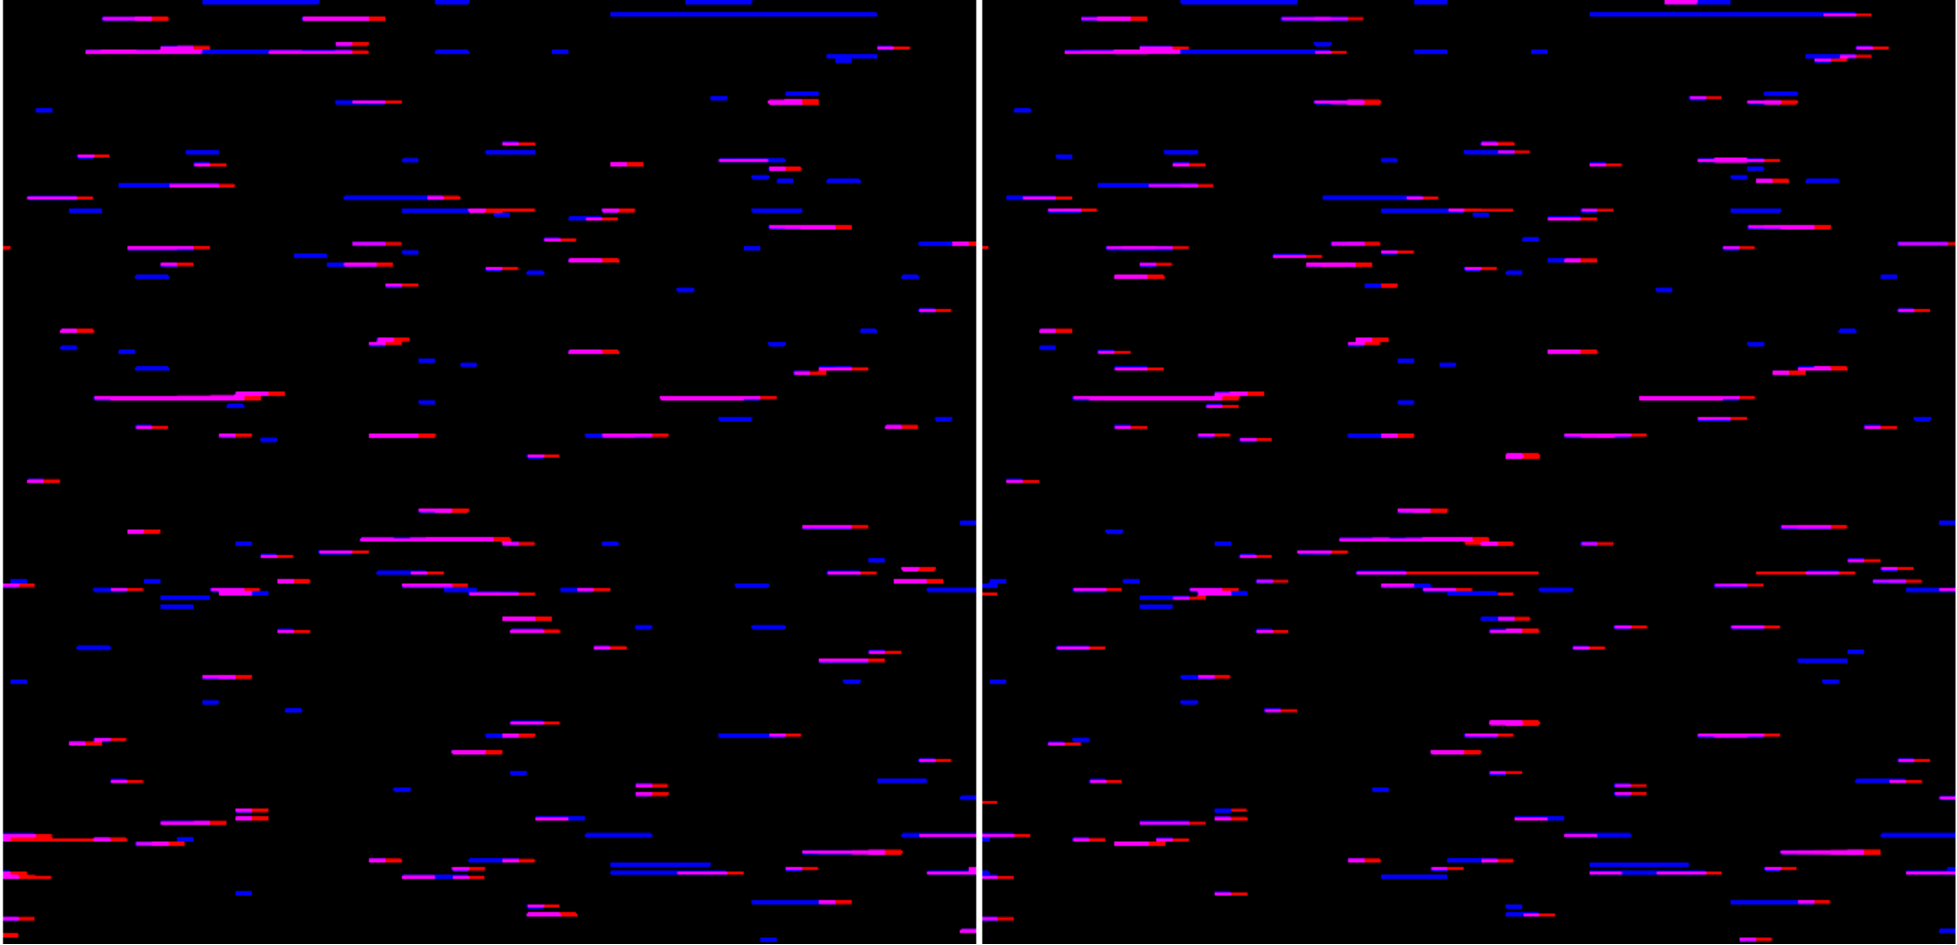
\includegraphics[width=.9\linewidth]{../images/plots/xeqcyv_kafka_heatmap_beginning_end.pdf}
\caption{\label{fig:org8be3697}
Address-visitation heatmap over the tomato-RT-N18U-httpd process memory, by the \emph{Xeqcyv} population, under the ``Kafkaesque'' fitness function: Season 4 on the left, Season 212 on the right. Blue swaths indicate where the harvested gadgets lie, red and magenta swaths indicate addresses visited by creatures in the population in execution.}
\end{figure}


The tendency of these populations to shrink from execution, as shown in figure
\ref{fig:org3b7bb3b}, is not at all surprising. The longer they spend in
execution, the greater their risk of crashing. Since crashing is the one \emph{sure}
way to draw selection's wrath, the population is highly disincentivized to spend
any longer than they have to in execution. There is simply nothing for an
individual under such selective pressures -- and only those -- to gain by
running code on the \gls{cpu}. There is no ``task'' to be completed in this setup,
after all. Computation, for the creatures of \emph{xeqcyv} and \emph{kurlig}, it essentially
vestigal, and rapidly atrophies. And so execution times contracted to as little
as 4 instructions on average, with much less variation than seen in the
\emph{Kurlig} population.

\subsection{Preparing an execv() system call in the Tomato web server}
\label{sec:org050fe87}
\label{org753cc2a}

In the experiments discussed here, we targetted the \gls{http} daemon extracted from
the firmware binary of a popular, open-sourced \gls{arm} router, with the filename
\texttt{tomato-RT-N18U-httpd}, and focussed on preparing a call to \texttt{execv()}. This binary
has the fortunate (for us) property of not only containing a considerable number
of gadgets, but several hardcoded path strings as well. \texttt{\#!/bin/sh} sits comfortably
at address \texttt{0x0001bc3e}, for example -- though it is terminated by a newline (\texttt{0x0a}),
and not by a null byte. Another interesting string that we can find there, residing
at address \texttt{0x0001f62f}, is \texttt{"/tmp/flashXXXXX"} -- just a few hundred bytes below an
apparent error message, reading \texttt{"Unable to start flash program"}. It appears that
the \texttt{XXXXXX} suffix is overwritten at runtime, at some point, yielding a valid path
to an executable, which, presumably, reflashes the router and restores factory
settings\footnote{This conjecture warrants a bit more reversing than I've carried out so far,
  but in the meantime this works as a plausible scenario, which is all we need
  for this PoC of \gls{roper}.}. And, just as we'd expect, the pathname, along with \texttt{/bin/sh}, resides in 
\emph{writeable} memory. The resources for exploitation are numerous here, and the
situation is ripe for \gls{roper}'s exploration.

To get our proof of concept underway, we'll set out \gls{cpu} state pattern string,
which \gls{roper} will parse and use to parameterize its fitness function, to
\begin{verbatim}
0001f62f,&0001f62f,00000000,_,_,_,_,0000000b
\end{verbatim}
Each comma-separated cell in the string represents a register. The underscores indicate
registers that we don't care about for the purpose of this task, and they will be
ignored by the fitness function. The ampersand is the indirection operator, as in C, 
and it tells \gls{roper} that \texttt{R1} should contain a \emph{pointer} to the address of the
string, ``/tmp/flashXXXXXX'', which, for its part, is known to reside at \texttt{0x1f62f}. 

A satisfactory \gls{cpu} pattern was soon produced by an individual in the \emph{wiwzuh} 
population, seventeen genealogical steps from the initial population. This specimen
isn't particularly complex, once you factor out a few of the detours it takes. 
It essentially works by just popping the necessary values from the stack to the
registers -- all evolution needed to do here was to find the values that 
hadn't been provided in the initial integer pool (such as the pointer\texttt{0xfff8} to the
value \texttt{0x1f62f}) and to place them in the necessary order. All that's needed in order
to actually launch this syscall is to place a single \texttt{SVC} instruction pointer
at the end of the packed chain shown in table \label{fig:wiwzuh}. The Tomato binary
has 859 to choose from, and the choice is more or less arbitrary. 

Even with so simple a task, the fitness landscape traversed by \gls{roper} displays
a surprising degree of ruggedness, as we can see in figure \ref{fig:org5ddc0d4}. 

\begin{figure}[htbp]
\centering
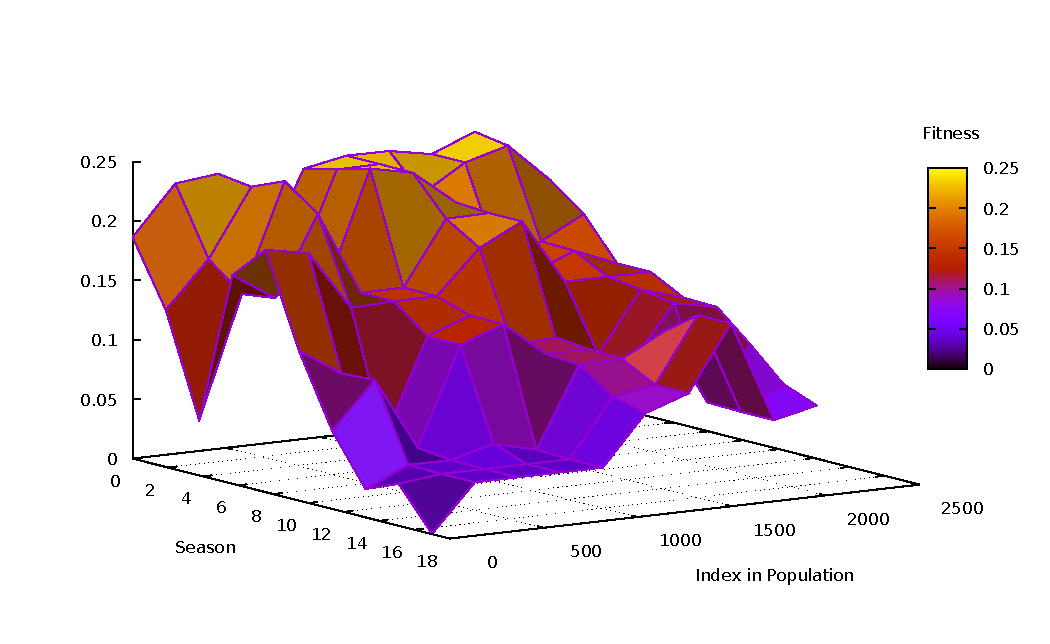
\includegraphics[width=.9\linewidth]{../images/plots/wiwzuh_syscall_gaussian_3.pdf}
\caption{\label{fig:org5ddc0d4}
Gaussian approximation of the fitness landscape across the population and over evolutionary time, for the \emph{Wiwzuh} population, evolving \texttt{execv("/tmp/flashXXXXXX", ["/tmp/flashXXXXXX"], NULL)} syscall \gls{rop} chains in tomato-RT-N18U-httpd, yielding a specimen with perfect (0.0) fitness.}
\end{figure}

\needspace{32}

\begin{table}
\label{fig:wiwzuh}
\begin{lstlisting}
(*\textbf{Clumps:}*)
[*] 0000b4ac   00000000   00000b17   0000000b   0000000b   00000000  
[*] 0000d1a0   0001f62f   0001f62f   0001f62f  
[*] 00016654   706d742f  
[*] 0001706c   0001f62f   0000fff8   0001f62f  

(*\textbf{Packed:}*)
ac b4 00 00  00 00 00 00  17 0b 00 00  0b 00 00 00  
0b 00 00 00  00 00 00 00  a0 d1 00 00  2f f6 01 00  
2f f6 01 00  2f f6 01 00  54 66 01 00  2f 74 6d 70  
6c 70 01 00  2f f6 01 00  f8 ff 00 00  2f f6 01 00  

(*\textbf{Execution Trace:}*)
0000b4ac        pop {r4, r5, r6, r7, r8, pc}

0000d1a0        cmp r0, #0
0000d1a4        popeq {r3, r4, r5, pc}

00016654        cmp r0, #0
00016658        ldr r3, [pc, #4]
0001665c        moveq r0, r3
00016660        pop {r3, pc}

0001706c        ldm sp, {r0, r1}
00017070        add sp, sp, #0x10
00017074        pop {r4, r5, r6, pc}

(*\textbf{Registers:}*)
R0:  1f62f->706d742f  R8:  0->68732e00 
R1:  fff8->1f62f      R9:  0->68732e00
R2:  0->68732e00      R10: 0->68732e00
R3:  706d742f         R11: 0->68732e00
R4:  0->68732e00      FP:  0->68732e00
R5:  0->68732e00      SP:  2b053->0   
R6:  0->68732e00      LR:  0->68732e00
R7:  b->746e692e      PC:  0->68732e00
\end{lstlisting}
\caption{A perfected \texttt{execv()} payload on \texttt{tomato-RT-N18U-httpd}, from the \emph{Wiwzuh} population, generation 17.}
\end{table}


\label{orgc1126db}
I must make a correction to a report stemming from this series of 
experiments that I had previously published and presented (\cite{fraser17_gecco}, 
\cite{fraser17_atlseccon}). I had initially set the target pattern for these attacks
to \texttt{02bc3e,02bc3e,0,\_,\_,\_,\_,0b}, where I had identified \texttt{02bc3e} as the address
of the string \texttt{"/bin/sh"} in the httpd binary. This was inaccurate on three counts:
first, the address was off by\texttt{ 0x10000} bytes, as a more careful inspection of the
program headers -- and subsequent improvement of \gls{roper}'s \gls{elf} loader --
revealed. Second, that string is not null-terminated, and so we'd have trouble
passing it as-is to \texttt{execv()} -- though it is newline-terminated, sitting at
the beginning of an embedded shell script, and residing in writeable memory, so 
it's still likely of some use, with a bit of manoeuvering. Most seriously, though,
was a rookie mistake I had made in relaying \texttt{execv()}'s signature: the second
parameter requires another degree of indirection, and so this particular payload
would have immediately resulting in a segmentation fault, if deployed in a real
scenario. These errors all stand corrected in the current document, and \gls{roper}'s
handling of pointer indirection and dereference has been vastly improved, along
with its \gls{elf} loader.


Some good nevertheless came from that oversight, as it called to my attention an
extraordinarily interesting and counterintuitive pattern in the behaviour of
many of \gls{roper}'s strongest specimens, which was thrown in sharp relief by
the champion chain of that particular run, system call bugs notwithstanding.
The specimen that caught my interest is reproduced here, in table
\ref{tab:labyrinthine}.


\subsection{Results of the classification problem}
\label{sec:org2625b05}
\label{org16c7cdd}

In what follows I describe some of the findings arrived at by experimenting
with assigning classification tasks to \gls{roper}. Two different datasets are
considered: an artificially simple and linearly separable dataset consisting
of two classes, and the well-known ``iris dataset'' by Fisher. But first, a few
remarks on the character of the problems we're looking at seem worth making. 


\subsubsection{Particular challenges imposed by ROPER's phenotypic landscape}
\label{sec:orga2d3d43}
\label{orga829c38}

Studying \gls{roper}'s handling of simple classification problems, where the
odds of success by any standard classification algorithm can be more or less
anticipated, throws into relief certain challenges that are peculiar to \gls{roper},
owing to the unusual terrain of the phenotypic landscape that it is forced to
traverse. The routes that it tends to carve out between problem and solution
are often extremely indirect and circuitous, due to pressures that are external
to the shape of the problem space, as specified in the data set, for example, but
internal to \gls{roper}'s operational semantics.

To begin with, of course, there is the constant threat of segfaulting, which is
never a concern for genetic programming systems that have been designed, from the
ground up, with their intended purpose in mind (assuming there are no bugs in the
implementation). \Gls{roper} must not only find a solution to each problem in the
problem set, but do so without throwing the \gls{cpu} into an exceptional state. At
the beginning of a run, \emph{most} execution paths lead to a crash, as may be expected
when executing randomly assembled \gls{rop} chains, on which very little prior
sanitization has been performed. A great deal of \gls{roper's} evolutionary time
appears to consist in winnowing useful components out of their unviable, crash-prone
encasings.\footnote{This is a conjecture based on indirect evidence, such as the frequency with which
  the ``minimum fitness'' measurement (the best performer, crashing aside) outpaces
  the ``best fitness'' measurement (the best, non-crashing performer), but more
  fine-grained collection of genealogical data, and further experimentation, is
  necessary for us to be sure that this is, indeed, a common tendency.} 


Furthermore, even without considering the probability skews caused by genetic drift,
there is an unevenness in the space of possible outcomes -- represented, for example,
by register states -- that is imposed by the materials that the host binary makes
available. Consider, for instance, the distribution in the frequency of register
usage shown in figure \ref{fig:orgd9bb420}. If the output registers
used for the bid-based classification function are, say, \texttt{R0}, \texttt{R1}, and \texttt{R2}, then,
all else being equal, we can expect to see the class designated by \texttt{R0} receive 
more attention, until the population calibrates itself.\footnote{At some point, this needs to ascertained through experimentation. For that, we'll
  need finer-grained information on the classification confusion matrices than the
  current version of \gls{roper} provides (since the focus has been on balanced data
  sets, the detection rate data has remained fairly coarse grained), but this should
  be simple enough to implement.}

\begin{figure}[htbp]
\centering
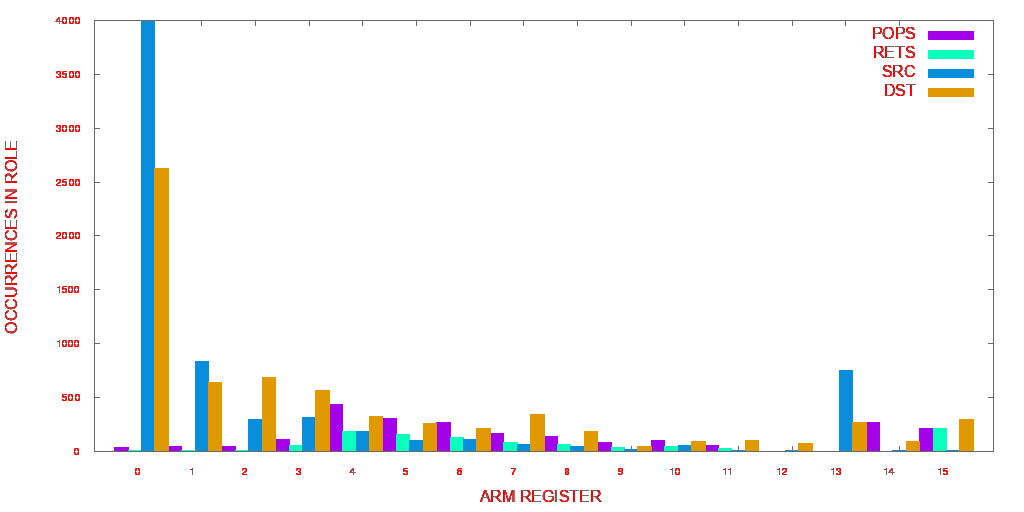
\includegraphics[width=.9\linewidth]{../images/plots/tomato-register-histogram.png}
\caption{\label{fig:orgd9bb420}
Register use histogram for the tomato-RT-N18U-httpd \gls{arm} \gls{elf} binary, used in many of the experiments documented here. The general shape of this distribution is representative of all of the \gls{gcc} compiled \gls{arm} \glspl{elf} I have looked at. The height of each bar represents the frequency with which the register, indexed on the X-axis, appears in pop-type instructions, in returns, and in the source and destination of data manipulation instructions.}
\end{figure}

At the present time, no explicit adjustment is made to the fitness functions
to account for this uneveness, though the \emph{difficulty} mechanism and its use in
fitness sharing (see \S \ref{org48435b5}) provides a means for the evolutionary
process to, eventually, gain some traction on it.

These qualities should be borne in mind when assessing \gls{roper}'s performance
on the following classification tasks. Its performance is in no way impressive,
when compared to any standard classifier implementation, and these results are
not intended to showcase \gls{roper}'s merits \emph{as} a classifier. They're put
forward as a proof of concept, demonstrating, by construction, that anything as
strange and improbable as \emph{training a population of \gls{rop} chains to recognize
patterns in data} is possible.

\subsubsection{Classification of a simple, linearly separable dataset}
\label{sec:orgcc99359}
\label{orgbae8b45}

As a way of establishing the minimal feasibility of performing classification
tasks with \gls{roper}, I tested the system with an extremely simple, linearly
separable dataset that I had generated artificially, with just two attributes
and two classes (see figure \ref{fig:org60e6ba3}).

\gls{roper} had very little difficulty with this problem set, and was able to
generate fairly good classifications of the data in the initial trials (figure 
\ref{fig:org6efa3be}). Its best specimen clearly relied on a single
attribute in forming their classifications -- basing them, it appears, on the
sign of the \(x\) parameter -- but it seems likely that some fine-tuning of the
(currently very naive) fitness function should be able to encourage a subtler
approach. A fine-tuning of the fitness sharing parameters would perhaps be
sufficient to draw selective pressure's attention to the two blue points
misclassified as red.

\begin{figure}[htbp]
\centering
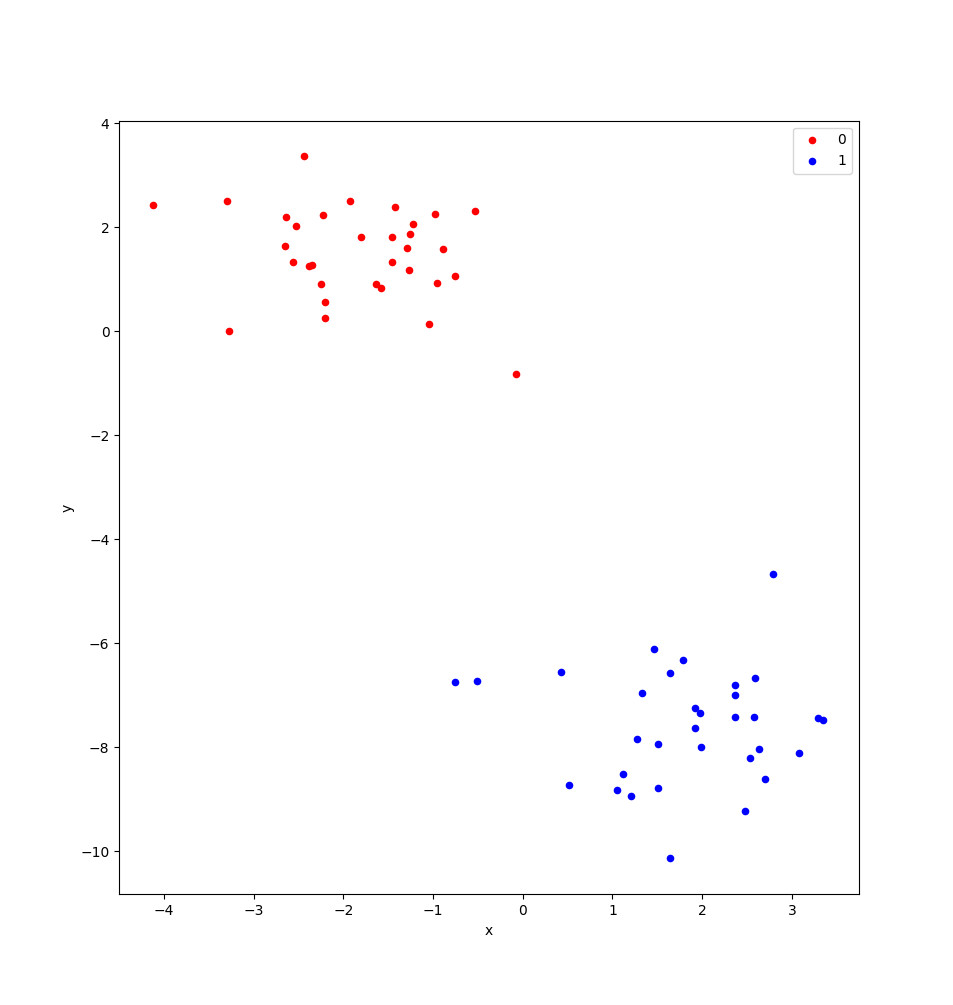
\includegraphics[width=.9\linewidth]{../images/plots/2_simple_blobs.png}
\caption{\label{fig:org60e6ba3}
An extremely simple, artificial data set, with two linearly separable classes determined by two points.}
\end{figure}

\begin{figure}[htbp]
\centering
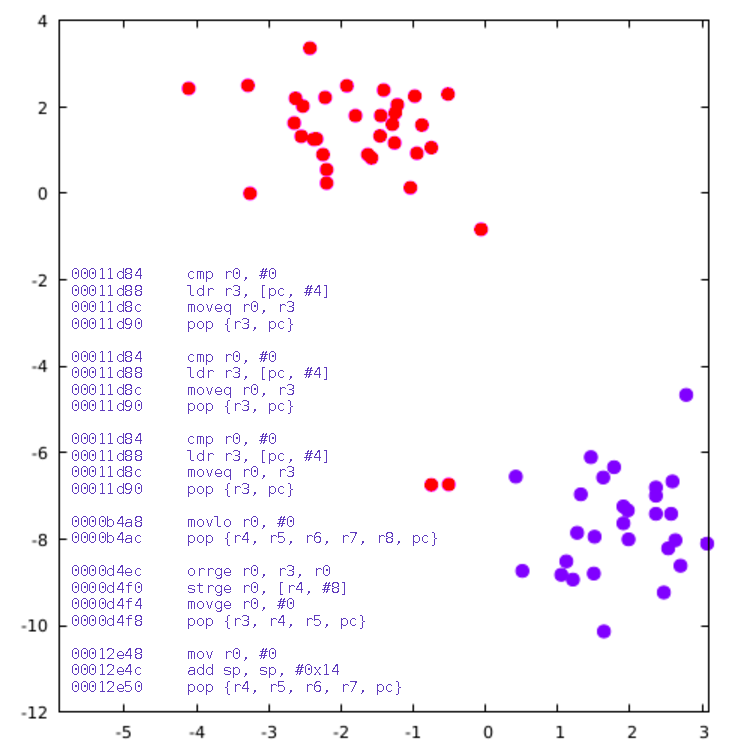
\includegraphics[width=.9\linewidth]{../images/plots/kathot_champion_18916_blobs_disas.pdf}
\caption{\label{fig:org6efa3be}
The classification on the data displayed in figure \ref{fig:org60e6ba3} performed by the best specimen in the \emph{Kathot} population, 35\(^{\text{th}}\) generation (execution trace inset).}
\end{figure}

\begin{figure}[htbp]
\centering
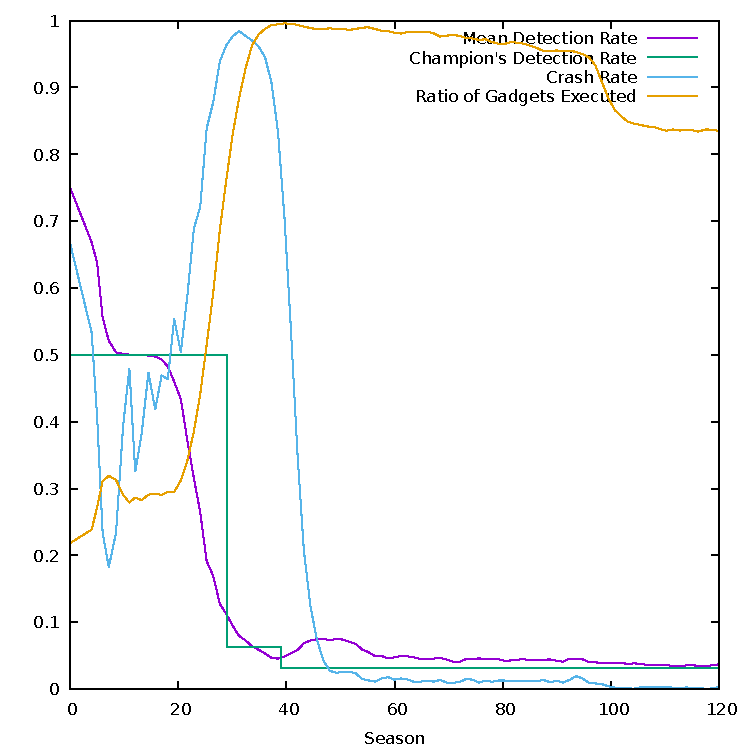
\includegraphics[width=.9\linewidth]{../images/plots/kathot_fitness.pdf}
\caption{\label{fig:org8b1417d}
Performance profile of \emph{Kathot} population, with gadgets in tomato-RT-N18U-httpd, on the ``two simple blobs'' classification problem.}
\end{figure}

\paragraph{A case study of malignancy in the \emph{Fizwej} population}
\label{sec:orga2a0047}
\label{orgc22774b}

Meanwhile, in the \emph{Fizwej} population, a genetic strain emerged that had found
a way to classify the simple dataset flawlessly -- or nearly so. Though it 
had achieved an error rate of 0.0, it terminated its execution, every time, 
with an instruction that caused the \gls{cpu} to crash with a write access violation.
This specimen illustrates a difficulty encountered often in \gls{roper} populations:
the offending instruction was part of the same gadget that did most of the work
in solving the classification problem, which can be reduced to the following sequence
of instructions, given some loose constraints on the constant popped into \texttt{R4}:
\lstset{language=asm,label= ,caption= ,captionpos=b,numbers=none}
\begin{lstlisting}
0000acf4    lsr r2, r4, #5            ;; a    := r4 << 5
...
0000acac    add r3, r3, r2, lsl #2    ;; Blue := Blue + (a << 2)
0000ad00    and r2, r4, #0x1f         ;; Red  := r4 & 0b11111
\end{lstlisting}

After solving the classification problem with these instructions, the phenotype
has no possibility of avoiding the next instruction in the gadget:
\lstset{language=asm,label= ,caption= ,captionpos=b,numbers=none}
\begin{lstlisting}
0000ad04    stmib r1, {r4, sl}
\end{lstlisting}
This instruction increments the value in \texttt{R1}, dereferences it, and then attempts to write
the contents of \texttt{R4} and \texttt{R10} (i.e., the stack-limit register, \texttt{SL}) to that
address. In the memory space mapped for \texttt{tomato-RT-N18U-httpd}, however, the
only legally writeably region of memory is the space allocated to dynamic memory
(where the heap resides) and to the stack,
from addresses \texttt{0x28000} to \texttt{0x28fff} and from \texttt{0x29000} to \texttt{0x2cfff}, respectively.\footnote{A sneaky ``gotcha'' that crops up when converting permission flags between ELF
  binaries and Unicorn or QEMU images is that while ELF's permission bits have
  the same semantics as the Unix file permissions: \texttt{100} for read, \texttt{010} for write,
  and \texttt{001} for execute, Unicorn encodes its permissions the other way around:
  now, \texttt{100} is execute and \texttt{001} is read, while \texttt{010} is still write.}
In the 7289 different specimens recorded
from the \emph{Fizwej} population, by the time of its 64\(^{\text{th}}\) season, that had this
particular gene and that had activated it to achieve a perfect detection rate 
on ``two simple blobs'', not a single one had managed to reliably dereference
\texttt{R1} to a writeable address at the time it dispatched that fatal instruction. 
To do so, indeed, they would have had to had changed their calculation strategy
entirely -- their entire \emph{modus operandi} consisted in setting \texttt{R1} to a negative
value when the exemplar belonged to the \textbf{red} class, and to a positive value when
it belonged to the \textbf{blue}, leaving \texttt{R0} more or less constant. All of the writeable
addresses in the process space, however, fall within the positive range mentioned.
The crash rate of this population rapidly reached 100\%, driving itself into an
evolutionary dead end. 


\begin{center}
\begin{tabular}{lll}
Start Address & End Address & Protections\\
\hline
\texttt{ 0x00000000} & \texttt{ 0x00000fff} & READ\\
\texttt{ 0x00008000} & \texttt{ 0x00020fff} & READ \(\vert{}\) EXEC\\
\texttt{ 0x00028000} & \texttt{ 0x00028fff} & READ \(\vert{}\) WRITE\\
\texttt{ 0x00029000} & \texttt{ 0x0002cfff} & READ \(\vert{}\) WRITE\\
\hline
\end{tabular}
\end{center}


\begin{figure}[htbp]
\centering
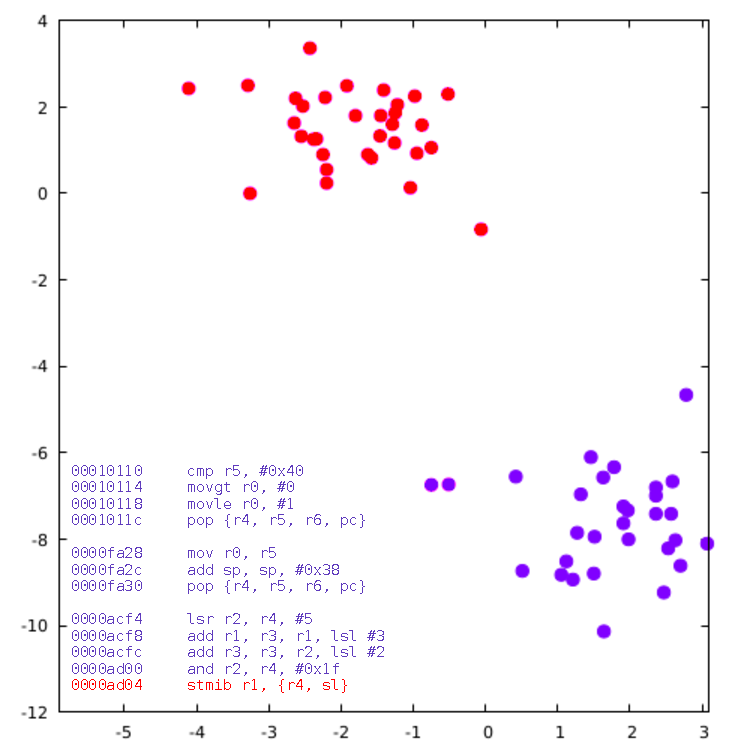
\includegraphics[width=.9\linewidth]{../images/plots/fizwej_perfect_crash.pdf}
\caption{\label{fig:org35724ba}
A genetic union of a harmful phenotypic trait with an advantageous one, in the \emph{Fizwej} population. As before, gadgets are separated by blank lines.}
\end{figure}

\begin{figure}[htbp]
\centering
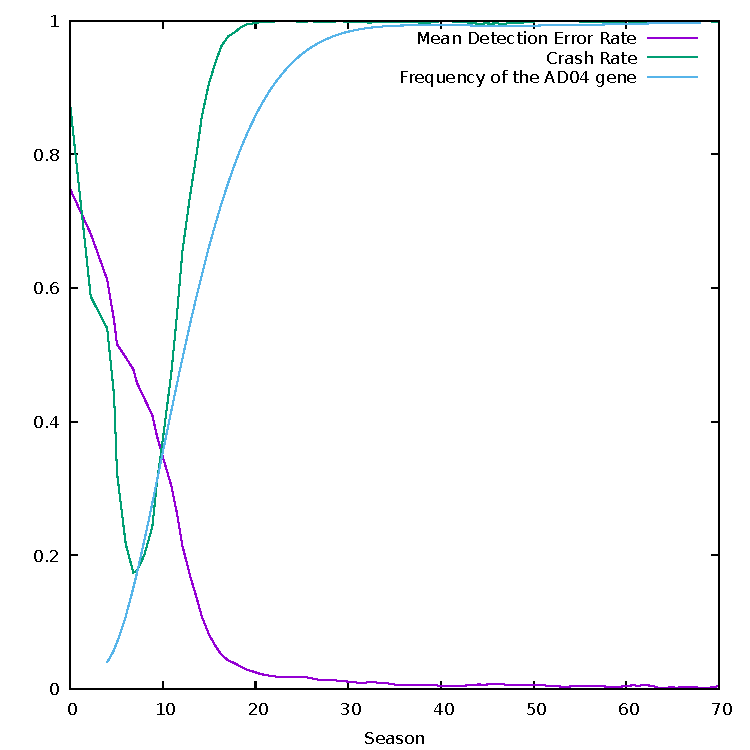
\includegraphics[width=.9\linewidth]{../images/plots/fizwej-badgenes.pdf}
\caption{\label{fig:org4d43759}
The evolutionary dead-end of the \emph{Fizwej} population, with the spread of the ``\texttt{0000ad04 stmib r1, \{r3, sl\}}'' gene.}
\end{figure}

\begin{figure}[htbp]
\centering
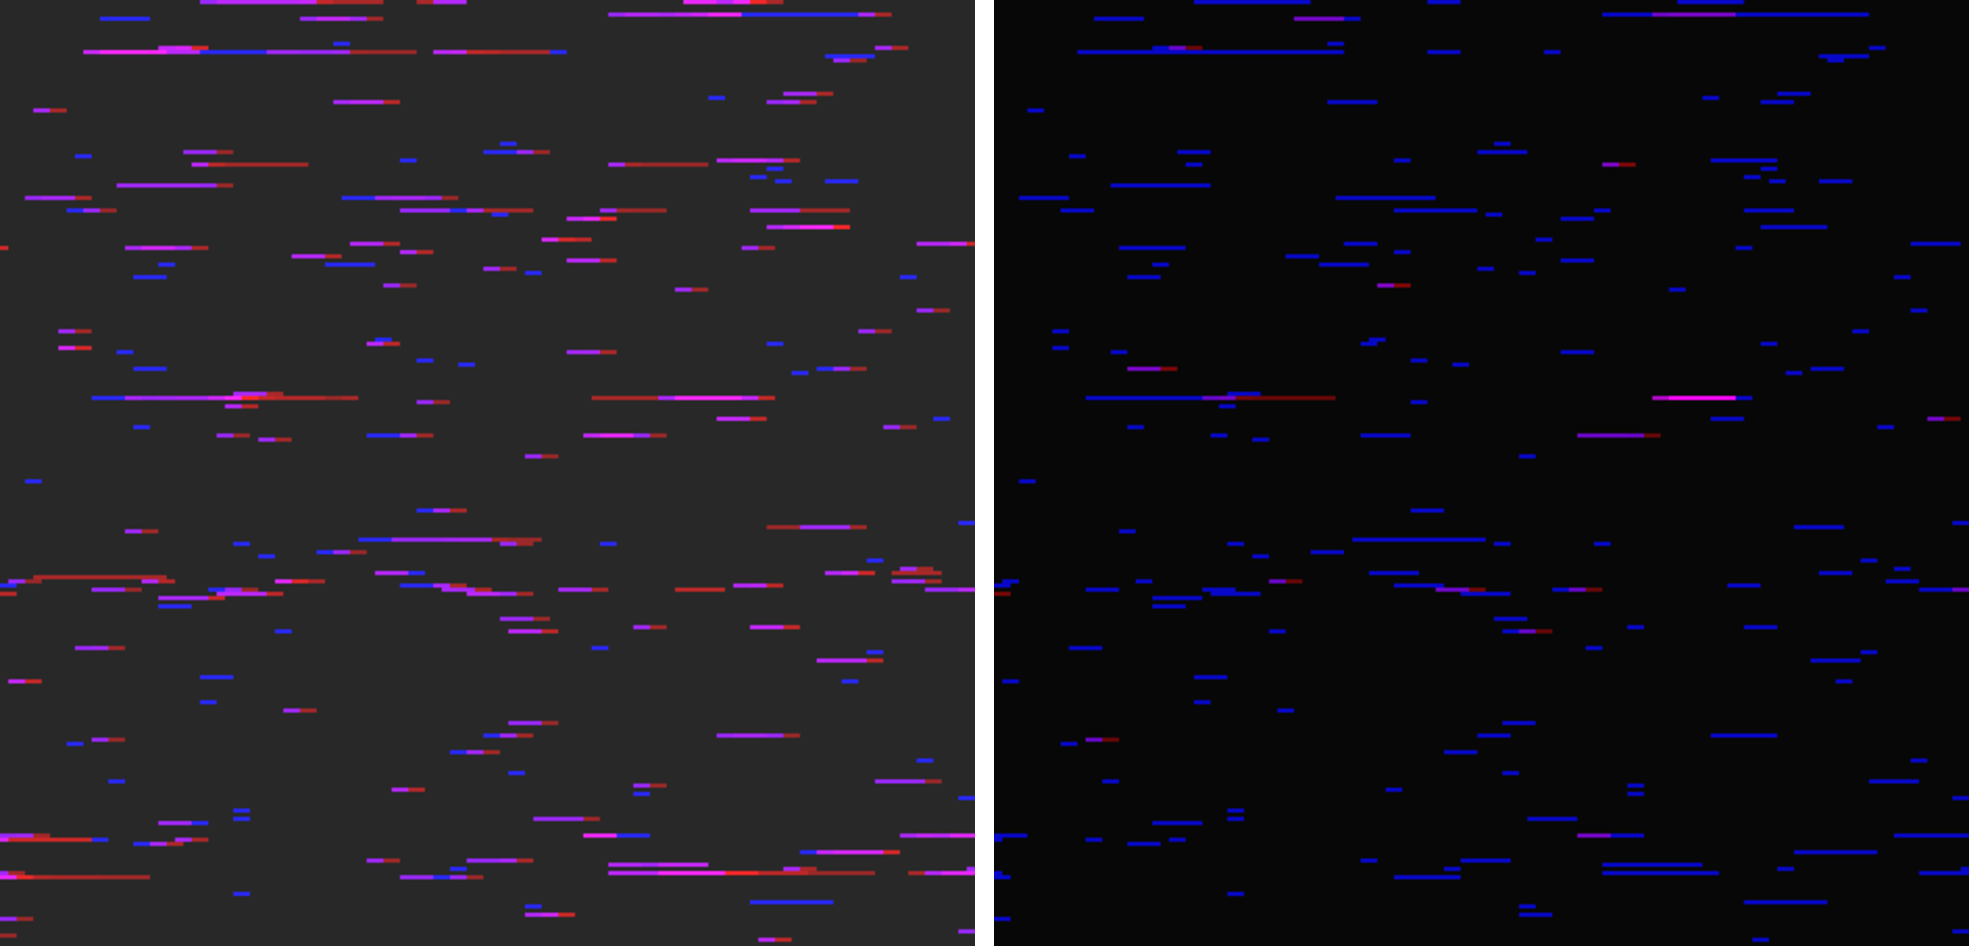
\includegraphics[width=.9\linewidth]{../images/plots/fizwej_S124_heatmap.pdf}
\caption{\label{fig:orged7bf36}
Address visitation heatmap of the \emph{Fizwej} population, at season 4 on the left, and season 124, on the right, showing a dramatic decline in phenotypic diversity. Compare with the \emph{xeqcyv} and \emph{kurlig} heatmaps in figures \ref{fig:org8be3697} and \ref{fig:orgaaeefc2}.}
\end{figure}

The obstacle that we're encountering here is that, owing to the complex structure
of the virtual instruction set that \gls{roper} is working with -- an instruction set
made up of gadgets rather than single machine instructions -- it is possible, perhaps
even common, for a dangerous phenotypic trait to secure its place in the population
when it is genetically united with an advantageous trait. Of course, this isn't just
a problem for \gls{roper}, but for biological organisms as well -- we see something
similar, for example, in the relation between malaria resistance and sickle cell
anemia \cite{haldane49}.

The question of whether or not a particular gadget is malignant is highly
context-sensitive -- since crashes are most often brought about through a
register dereference and a subsequent attempt to either read from, write to, or
execute data at an address for which the requisite permission has not been
granted -- and the pressures borne by selection are sometimes too coarse-grained
to answer it before a selective epidemic occurs. It may be interesting to
attempt to incorporate a more sophisticated semantic analysis routine to inspect
gadgets that trigger a crash, and to determine whether or not they should be
removed from the gene pool -- an idea we will take up further in the discussion
of future directions for this project, in \S \ref{orgca86428}. Incorporating
a gauge of genetic, or low-level phenotypic, diversity into the fitness function
-- scaling fitness by the relative frequency of either the individual's
machine-word composition, or its execution path through process memory -- may
also help mitigate the threat of malignant genetic convergence.

\paragraph{An early encounter with a segfault plague, due to an vulnerability in the crash handling mechanism}
\label{sec:org3d94838}
\label{org9a8c521}

\begin{figure}[htbp]
\centering
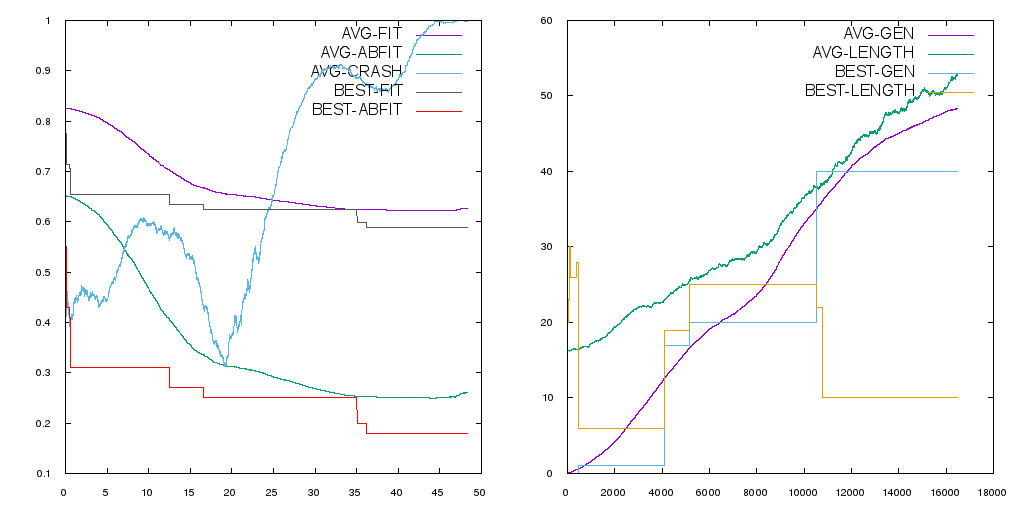
\includegraphics[width=.9\linewidth]{../images/plague.png}
\caption{\label{fig:org088e5df}
A plague of segfaults: the cyan line indicates the crash rate, and the lower left index shows the average genealogical generation, and not the number of iterations, as used in later graphs. The raw data for this experiment has unfortunately been lost, leaving only this artifact as a historical curiosity.}
\end{figure}

This wasn't the first time that I had seen a segfaulting strain rise to
dominance in one of \gls{roper}'s populations. In one, particularly fascinating
and unusually pathological trial with the Iris classification problem (which we
will look at more closely in \S \ref{org79793df}) , which I stumbled
across early in the experimentation, the crash rate skyrocketed, and the \emph{entire
population} fell victim to a congenital plague of segfaults before its
20,000\(^{\text{th}}\) tournament iteration (figure \ref{fig:org088e5df}). Due to the data that
was collected at the time being insufficiently coarse-grained, I cannot say
whether dynamics similar to those described in \S \ref{orgc22774b} played
a role in this occurrence. At least one of the factors leading up to it was
uncovered, however, by reviewing the mean ``ratio run'' metric of the population:
the population had discovered a means of exploiting the sloppy implementation of
the gadget-return counter, which was responsible for tracking how many gadgets
had executed before a crash occurred, that was then in effect. New to the
Unicorn library and the Rust language, and somewhat frustrated with the
complications involved in having a callback to the Unicorn engine soundly pass
data back to the Rust context from which the engine was dispatched, I'd taken a
shortcut and built a counter in what I expected would be an unused region of the
emulator's memory space, and then used a straightforward API to read the counter
from memory after execution had terminated. At the time, I imagined that though
there was some chance the counter could \emph{perhaps} get corrupted, I would be able
to treat that corruption as inconsequential noise. This was a mistake, and the
population wasted no time in exploiting it. A dominant genetic strain had
evolved to hijack the return counter, setting it to an artificially high value
before wantonly crashing. The apparent success of those chains in executing
numerous gadgets before crashing meant had reduced the crash penalty to near
zero, and since enough of this line had managed to perform fairly well on the
classification task -- achieving an 82\% detection rate against Iris -- in
addition to exploiting the experimental framework, they soon wiped out every
single lineage that they ran up against.\footnote{This was a very nice example of
what Lehman et. al have called ``The Surprising Creativity of Digital Evolution''
in \cite{lehman18}.}

This was by no means the norm, however. The bug was fixed, and a secure conduit
for the return counter was implemented, avoiding any in-band communication that
could be hijacked by the population it was meant to assess. As an additional
safeguard, a second factor was incorporated into the crash-penalty gradation:
the penalty would steepen in proportion to the global frequency of crashes in
the population. 

This bolstered the tendency of the crash rate to oscillate, of course, though
the oscillations appear to occur to some degree with or without the global
crash frequency penalty. The global crash rate would generally settle into
a comfortable oscillation between 1 and 20 percent of the population crashing,
at any given time. 

A stricter penalty could easily reduce the crash rate to almost zero, but
this appeared to negatively impact long-term performance. The fitness landscape
inhabited by \gls{roper}'s populations, it seems, is extremely jagged, and
too strict a penalty to crashing would prevent the population from crossing 
from one fitness peak to another. It made more sense to work with the tendency
for crash rates to oscillate than against it, and allow exploration of more
dangerous waters so long as it doesn't threaten to risk the long-term well-being
of the population as a whole. 

In view of the phenomena described in \S \ref{orgc22774b}, however, this approach to regulating the crash rate may warrant revision. 

\paragraph{A proposed method for regulating malignant genes with a TTL field}
\label{sec:org923b21d}
\label{orgb6dff3e}

Another mechanism that we could use to mitigate this dynamic may be to add
a \gls{ttl} field to our \texttt{clump} datatype. With each crossover or cloning event, 
the \gls{ttl} would be decremented, and when it reaches zero, the clump would be
excised from the genome and replaced with a new, randomly generated one, perhaps
with an identical \gls{spd} and immediate component. In the event of a crash, we
could examine the address visitation path tracked by the emulator to find the 
last clump entered before crashing. Once the guilty clump is found, its \gls{ttl}
could be halfed (or some order of magnitude greater than the linear decrement
that occurs in crossover). We could then experiment with the results of different
tunings to the \gls{ttl} field and its methods, and see if this might be a better
way of regulating the crash rate than the current approach, which simply factors
a crash penalty into the same, scalar fitness value that determines reproductive
odds. 


\subsubsection{\emph{Fleurs du malware}: Classification of the Iris data set}
\label{sec:orge894a2d}
\label{org79793df}

The Iris dataset, though relatively simple by contemporary classifier standards, 
is considerably more complex than the ``two simple blobs'' dataset explored in
Section \ref{orgbae8b45}. Its attribute-class mapping is plotted
in figure \ref{fig:org71c6a67}

\begin{figure}[htbp]
\centering
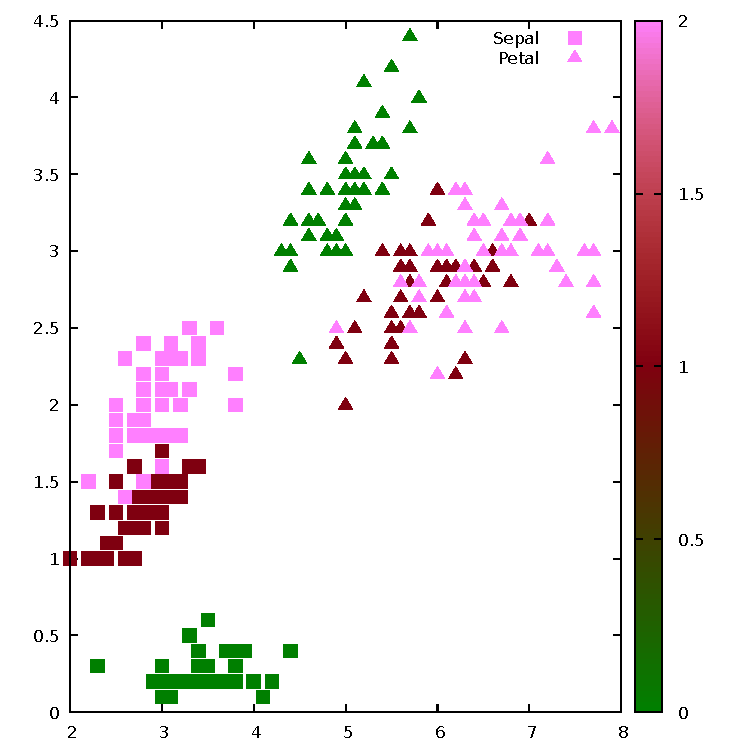
\includegraphics[width=.9\linewidth]{../images/plots/iris_plot.pdf}
\caption{\label{fig:org71c6a67}
Map of the Iris dataset. Triangle points represent petal measurements, and square points represent sepal measurements, with length on the X-axis and width on the Y-axis. Colour maps to species: green for \emph{setosa}, maroon for \emph{versicolor}, and pink for \emph{virginia}.}
\end{figure}


\paragraph{Without fitness sharing}
\label{sec:org992c74a}

The fitness curve of our best specimens \emph{without fitness-sharing} typically took
the form of long, shallow plateaus, against the backdrop of a population swaying,
it seemed, more in response to genetic drift than selective pressure.

An interesting phenomenon seemed to recur in several populations, however, following
a prolonged fitness plateau: long after it had been effectively quelled by selective
pressure, the rate at which individuals crash during execution would begin to rise
again, climbing, in fits and starts, from near zero to up to 40\% of the population.
This is what we see happening in figure \ref{fig:org0b79203}, for example,
which documents one of the early experiments performed with \gls{roper}.

\begin{figure}[htbp]
\centering
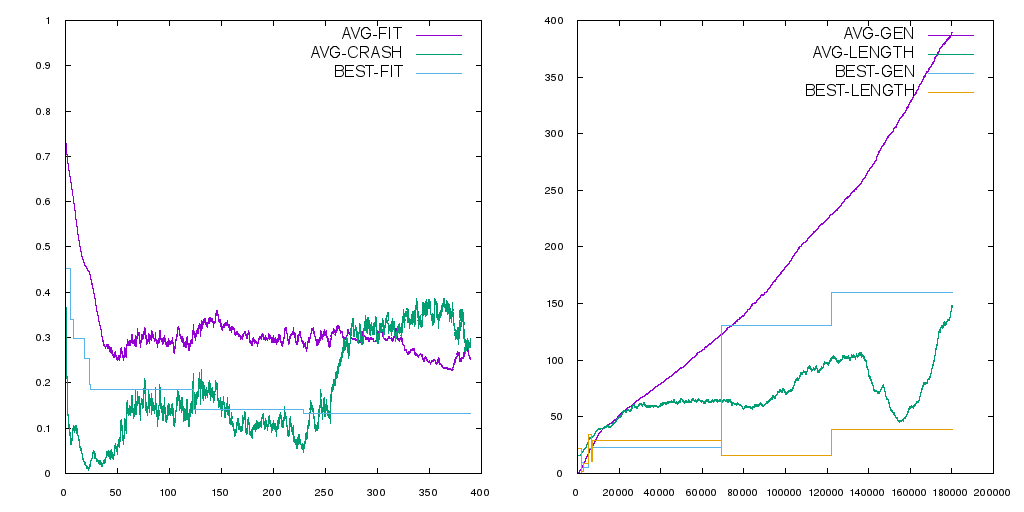
\includegraphics[width=.9\linewidth]{../images/plots/good-nosharing.png}
\caption{\label{fig:org0b79203}
Resurgence of the crash rate during a fitness plateau, in an early run of the Iris classification task, before implementing fitness sharing. The X-axis in the left-hand pane tracks the average generation of individuals, while the X-axis on the right tracks iterations of the main loop. The relation between the two measures is linear, and so these panes can be more or less superimposed.}
\end{figure}

One possible explanation for this strange behaviour is that a second-order selective
pressure encourage intron formation, of which the crash rate may be a symptom,
if the method for forming introns, favoured by this population, involved individuals
altering their own call stacks so as to escape dependency on certain segments of their
genomes -- a strategy that might be viable for one or two generations, but may result
in more fragile chains in in subsequent ones. I explore this possibility in more
depth in section \ref{orgc385372}.

Curiously, the peak in crash rate coincides with a dip in the average length of the
population, which appears contrary to the supposition that the population was undergoing
a strong pressure for intron formation at this point -- code bloat is almost certainly
the \emph{simplest} means of forming introns. This may be an artefact of the fragility
mechanic detailed in \S \ref{org7016026}, however: a sufficiently fragile gene
has a strong likelihood of simply being dropped during crossover, and passed to neither
offspring, and when a crash occurs, the fragility of the last gadget to have been
executed is automatically maximised. We could, therefore, be seeing a \emph{consequence}
of the rising crash rate in the corresponding drop in genome length -- this does, at
least, appear to me to be a likely hypothesis.

Another, non-exclusive possibility is that the fitness plateau we can see,
stretching across the second half of the history documented in figure
\ref{fig:org0b79203} is a symptom of (premature) genetic convergence. 
Perhaps it converged on a fitness peak that was robust enough to survive
a certain number of reproductive cycles -- long enough for it to establish
dominance in the population, and drive out competing phylogenic strains, but 
which was surrounded on all sides by steep ravines. By the time we start to reach
mean generation 220 or so, descendents of that strain may be starting to reach
the edges of that fitness plateau, and \emph{their} descendents begin dropping off the
edge, en masse. This seems incongruous with the mean fitness line continuing to
progress, but this is just the mean, and may be the effect of that strain completing
its ill-fated domination of the gene pool.\footnote{The raw data from this run has unfortunately been lost, and so we're restricted
  to speculating on the basis of its surviving artefacts.}

\paragraph{With fitness sharing}
\label{sec:org1ba4580}
\label{orgf62a73d}

 What would consistently seem to occur in the classification runs performed
 using a static fitness function, keyed to detection rate, was that the
 strains in the population would emerge that could reliably distinguish the
 linearly separable species of iris from the others, but whose competence
 would end there. This is, of course, not a trivial accomplishment in itself
 for a randomly generated \gls{rop} chain, and so this strain would rapidly
 outperform its competitors in almost every tournament in which it was
 represented, soon dominating the gene pool, and bringing about a genetic
 convergence of the population, whose performance would then plateau. If there
 had been any resources in the population that \emph{could} have made some headway
 on distinguishing the two less tractable, and more entangled, species, had
they had time to be tuned by genetic operators, those resources would likely
have been expunged by the gene pool in their carriers' fierce competition with
the ``bottom feeders'' whose high absolute fitness scores represented only a
facility for solving relatively \emph{easy} problems.

\begin{figure}[htbp]
\centering
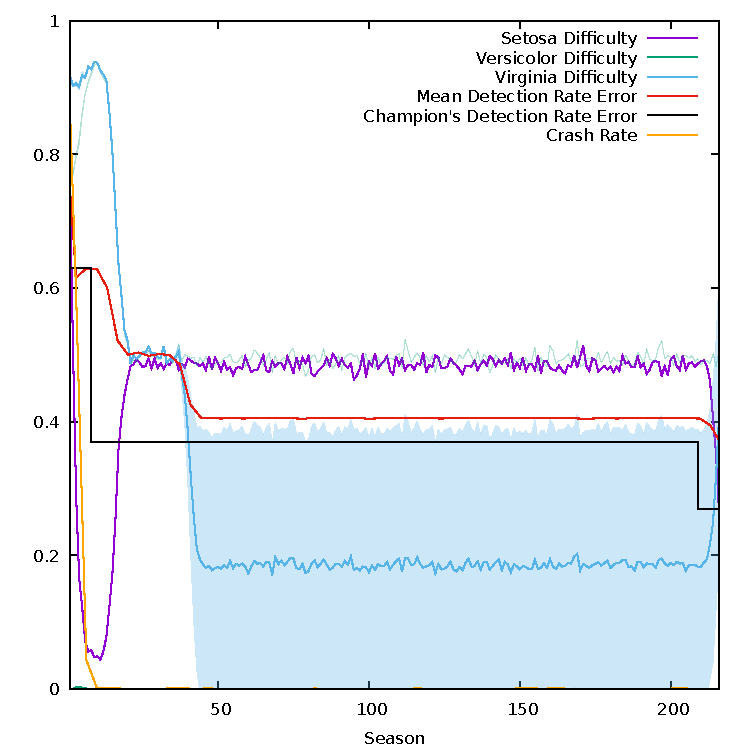
\includegraphics[width=.9\linewidth]{../images/plots/nosharing.pdf}
\caption{\label{fig:orgda24b66}
A trial similar to the one documented in figure \ref{fig:org2277148}, with per-class difficulty recorded, but with the fitness sharing mechanism suspended (\emph{Cazmud} population). The filled curve surrounding each mean difficulty class, here being of visible breadth only in the case of the \emph{iris virginia}, represents the standard deviation of difficulty for each exemplar class.}
\end{figure}

For this reason, I introduced into \gls{roper} the \emph{fitness sharing} mechanism 
that I have outlined in \S \ref{org48435b5}. 
 The result (after some persistence and plenty fine-tuning) was a superb run --
achieving 96.6\% detection rate (0.034 absolute fitness) on the Iris set in
27,724 tournaments, 216 seasons of difficulty rotation, and an average
phylogenic generation of 91.3. Figure \ref{fig:org2277148} shows the course the
evolution took, with the right-hand panel showing the responding environmental
pressures -- the \texttt{difficulty} scores associated with each class, showing both
mean and standard deviation.

\begin{figure}[htbp]
\centering
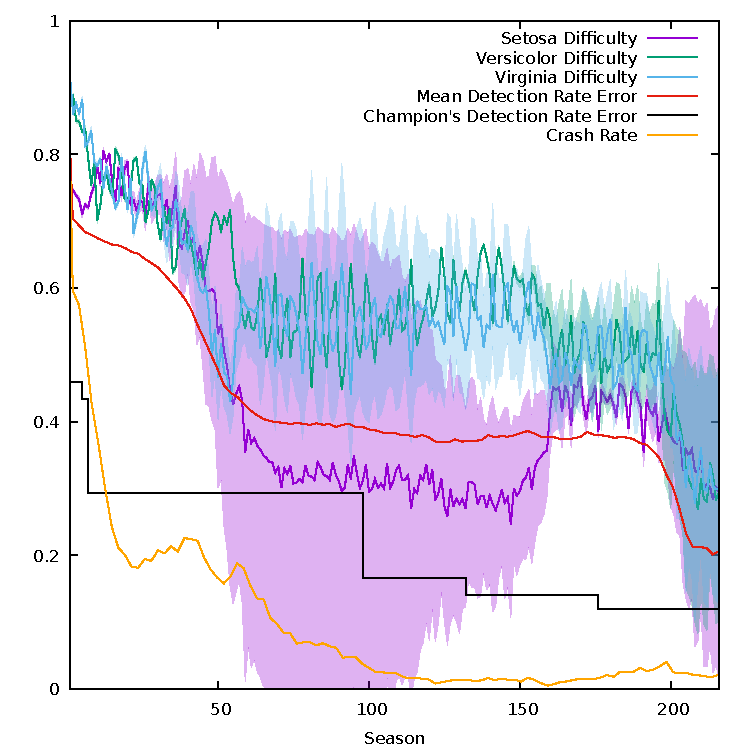
\includegraphics[width=.9\linewidth]{../images/plots/sharing.pdf}
\caption{\label{fig:org2277148}
A very good run on the Iris classification task, employing the fitness sharing algorithm documented in \S \ref{org48435b5} (\emph{Ragweb} population). The filled curve surrounding each mean difficulty line again represents the standard deviation of difficulty for that exemplar class.}
\end{figure}



This run can be informatively compared with the one illustrated in figure
\ref{fig:orgda24b66}. Note the tight interbraiding of problem difficulties in
figure \ref{fig:org2277148}, as compared to their gaping -- but still, slowly,
fluctuating -- disparity in figure \ref{fig:orgda24b66}. The ballooning standard
deviation of difficulty by class in figure \ref{fig:org2277148} also suggests
a dramatic increase in behavioural diversity in the population, which is
precisely what we aim for with the fitness sharing algorithm.


\subsection{Preliminary results of the \emph{Snake} experiments}
\label{sec:org609e67e}
\label{org28ee8f8}

In the final problem class put to \gls{roper}, I wrote a simple \emph{Snake} game
\cite{snakefight} for its populations to play, to see how they may respond to a
dynamically changing environment, with moderate to high degrees of randomness.
The specifications of the game are described above, in \S \ref{orgece58eb}.
To control the degree of randomness, I set up the game control protocol so that
the \gls{roper} engine could pass a random seed to the game in order to initialize
the placement of ``apples'' and ``cacti'' on the game board. Surprisingly, the 
system appeared to perform better when the seeds were randomly generated and
highly unique, rather than drawn from small set of seeds that would remain fixed
for the duration of the evolutionary run. 

Results on this experiment remain largely preliminary and anecdotal in nature,
but evidence of its basic feasibility can be found in the time-lapse recording
of the final champion of the \emph{Misjax} population playing a semi-competent game
of Snake in figure \ref{fig:orgd94fc0f}. 

\begin{figure}[htbp]
\centering
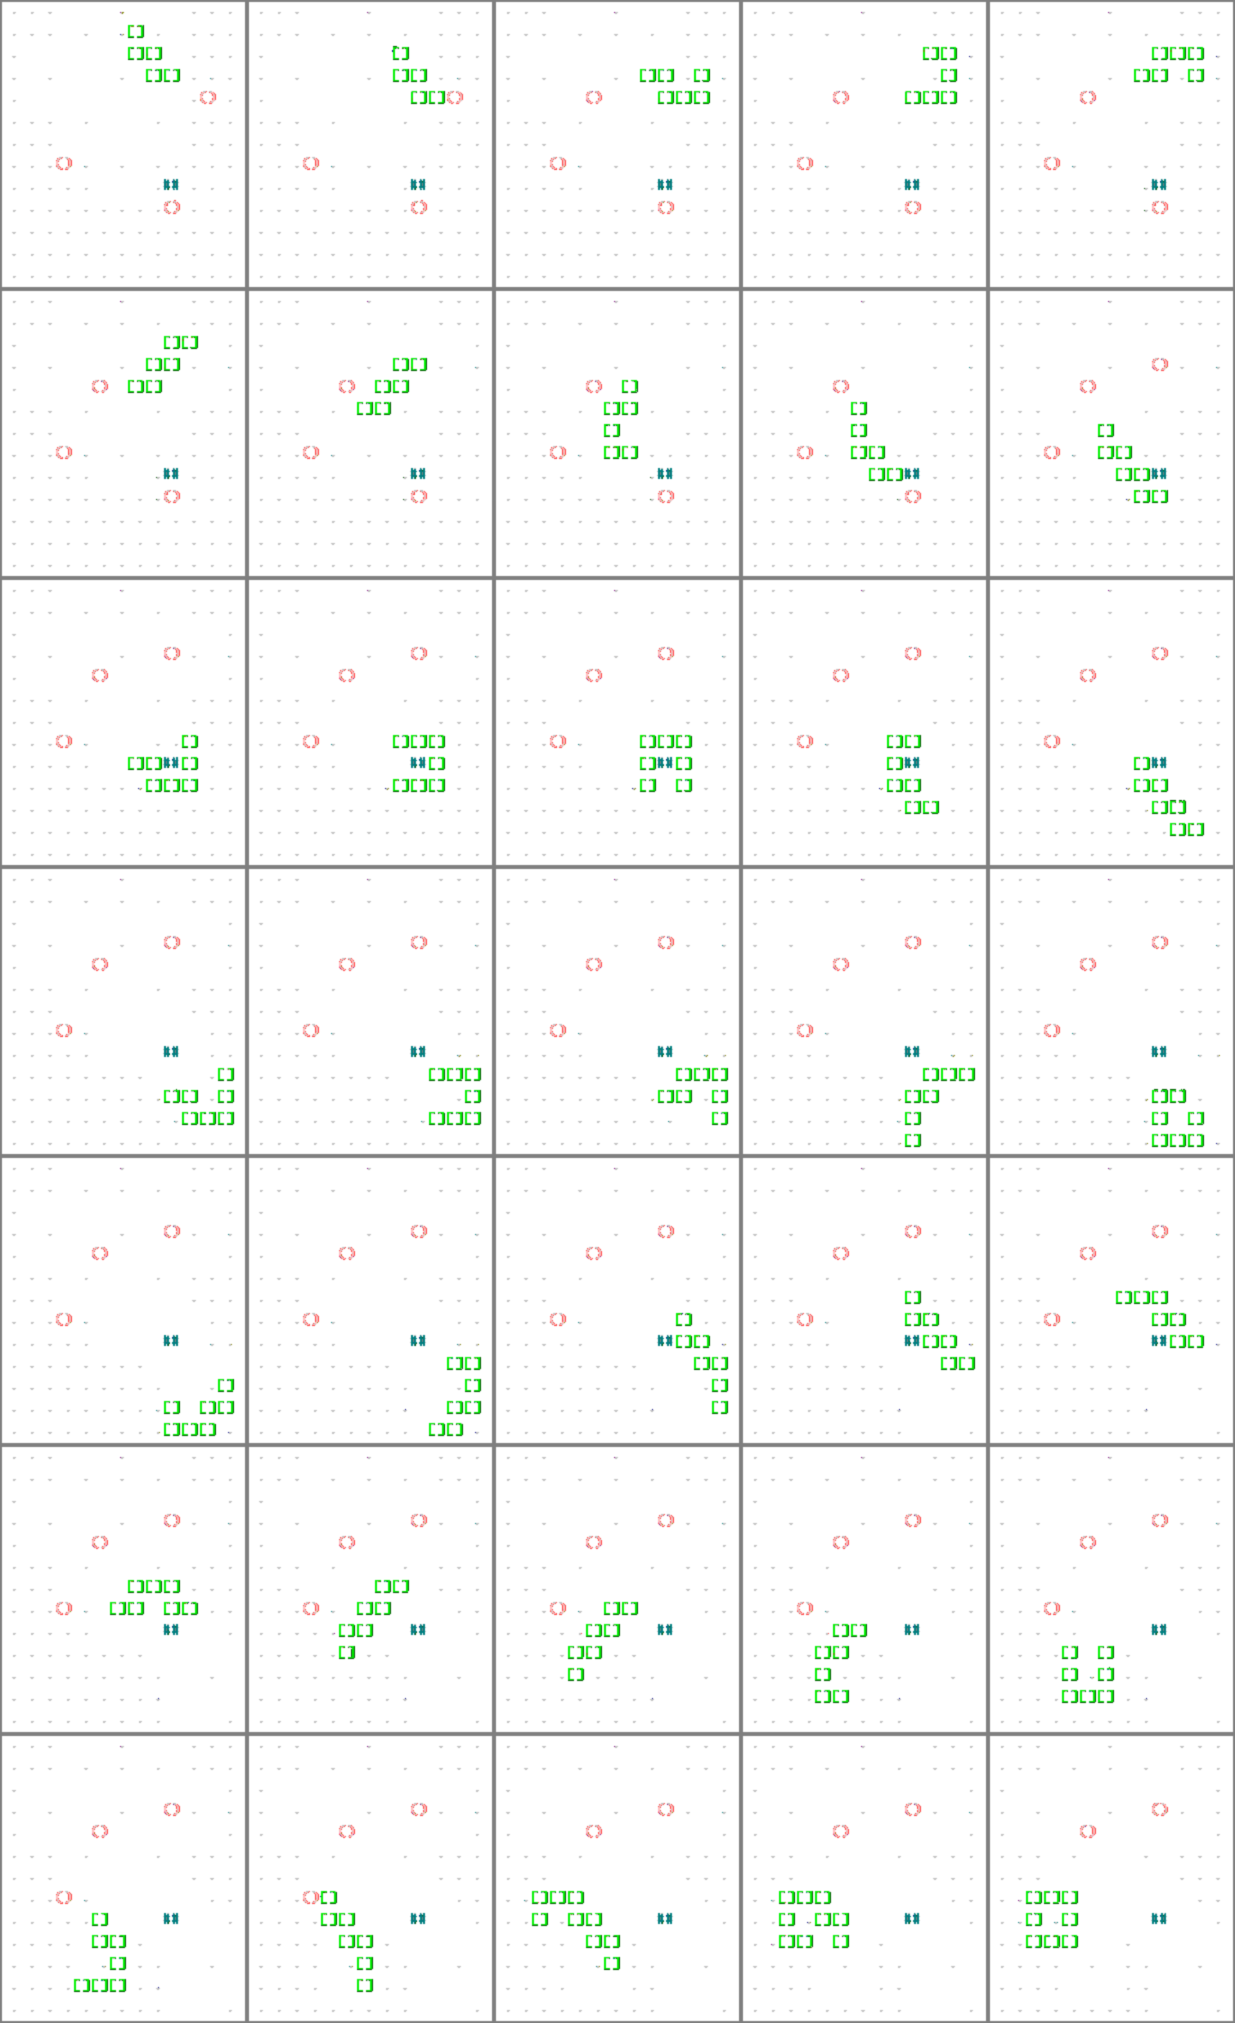
\includegraphics[width=.9\linewidth]{../images/snek_misjax_montage_on_white.png}
\caption{\label{fig:orgd94fc0f}
Time-lapse rendering of one of the fitter specimens encountered in the Snake trials (\emph{Misjax} population). Snake segments: \texttt{[]}, apples: \texttt{()}, cacti: \texttt{\#\#}.}
\end{figure}



\section{Intron Pressure, Self-Modifying Payloads, and Extended Gadgetry}
\label{sec:org6a40aec}
\label{orgd92d702}

In all of the experimental trials performed, a certain number of peculiar,
interrelated phenomena appeared in the dynamic behaviour of the population
as a whole. 

\subsection{Crash Rate Oscillations}
\label{sec:org2534500}
The first has to do with the observed crash rates. In the beginning -- as is to
be expected, since our initial gadget harvest is deliberately roughly hewn
and approximate, with no attempt to formally verify the individual reliability
or usefulness of each gadget or combination thereof -- the vast majority of our
specimens (80 to 90 percent) would crash before completing execution. This would
most often be the result of a segmentation fault, or memory access violation error,
when the specimens would attempt to dereference and invalid pointer, or jump to an
address outside of an executably-mapped segment of memory. Since such violations
carry with them a fairly steep penalty to individual fitness, \emph{and} increase the
likelihood that the genes responsible for exposing the individual to such hazards
are dropped from the gene pool, the rate of crashes would always drop fairly quickly
within the first few thousand tournament iterations. There is nothing unusual or
unexpected about this -- reducing the likelihood of crashing is the simplest way
for any of our individuals to ensure their survival and prospects of reproduction,
and appears to be much easier for our populations to accomplish than the specific
task-oriented components of the fitness function. And whereas the prospect of
crashing ``in the wild'', before having a chance to reproduce, is completely and
utterly fatal to evolving malware strains (see the discussion of this problem
in \S \ref{org48e63d9}), our ``in vitro'' populations have the advantage of a gently
gradated crash penalty: the fitness penalty incurred by a crash is inversely
proportionate to the number of gadgets viably executed before the crash.

What \emph{is} surprising, however, is that the crash rate does not \emph{continue}
to decline or stabilize at the extremely low level that it tends
to reach after its initial dropoff. The curve it traces relative to the
number of iterations doesn't even \emph{approximate} a monotonic reduction.
Instead, it eventually -- but consistently -- begins to rise soon after the
average fitness of the population reaches a plateau, and then starts to
oscillate, until the plateau is broken and the fitness equilibrium is
punctured. 

\subsection{The stray rate and extended phenotypes}
\label{sec:org706b1a8}
\label{orgc385372}

Once a secure conduit had been implemented for passing detailed execution
information from the emulator back to the evolutionary engine (see \S
\ref{org9a8c521},
another rich vein of information had opened up, which helped to provide evidence for a
tendency that, until then, I had only been able to observe by manually
dissecting the disassembly dumps of individual specimens post-mortem\footnote{As discussed in my \gls{gecco} 2017 report on this project \cite{fraser17_gecco},
  and my talk at AtlSecCon 2017 \cite{fraser17_atlseccon}.}: I had noticed a tendency for \gls{roper} populations' best
performers to frequently be those that take strange and enigmatic risks with their own
control flow -- manipulating the program counter and stack pointer directly,
pushing values to their own call stack, branching wildly into unexplored regions
of memory space, and so on. These are behaviours that seem, \emph{prima facie}, destined
for failure in most cases. Their apparent frequency was an enigma. 

Consider, for example, the specimen displayed in 
table \ref{tab:labyrinthine} which
achieved a perfect fitness in trial of the CPU context matching experiment,
where the task was to prepare the register vector for an
\begin{verbatim}
execv("/bin/sh", ["/bin/sh"], 0)
\end{verbatim}
system call -- the sort of task that manually crafted \gls{rop} chains are often
designed for, so that the attacker can spawn a shell with the privileges of the
exploited process.\footnote{See the semantic correction noted in \S \ref{org753cc2a}, which 
  spoils the real-world usability of this \emph{particular} chain, but which
  does not logically impact the analysis and conjectures formed here,
  in relation to it.}


\begin{table}
\label{tab:labyrinthine}
\begin{multicols}{2}
\begin{lstlisting}[basicstyle=\scriptsize\ttfamily]
;; Gadget 0 
000100fc         mov r0,r6 
00010100         ldrb r4,[r6],#1 
00010104         cmp r4,#0
00010108         bne #0xffffffb8 ;; = -0x48
0001010c         rsb r5,r5,r0 
00010110         cmp r5,#0x40
00010114         movgt r0,#0 
00010118         movle r0,#1 
0001011c         pop {r4,r5,r6,pc}

;; Gadget 1 
(*\color{violet}00012780~~~~~~~~~bne \#0x18*)
00012798         mvn r7,#0 
0001279c         mov r0,r7
000127a0         pop {r3,r4,r5,r6,r7,pc}

;; Gadget 2 
00016884         beq #0x1c 
00016888         ldr r0,[r4,#0x1c] 
(*\color{violet} 0001688c~~~~~~~~~bl \#0xfffffff0*) ;; = -0x10 
(*\color{red} 0001687c~~~~~~~~~push {r4,lr}*)
00016880         subs r4,r0,#0 
(*\color{violet}00016884~~~~~~~~~beq \#0x1c*)
000168a0         mov r0,r1 
000168a4         pop {r4,pc}

;; Extended Gadget 0 
00016890         str r0,[r4,#0x1c] 
00016894         mov r0,r4
00016898         pop {r4,lr} 
(*\color{violet}0001689c~~~~~~~~~b \#0xfffffdd8*) ;; = -0x228
(*\color{red}00016674~~~~~~~~~push {r4,lr}*)
00016678         mov r4,r0 
0001667c         ldr r0,[r0,#0x18] 
00016680         ldr r3,[r4,#0x1c]
00016684         cmp r0,#0 
00016688         ldrne r1,[r0,#0x20] 
0001668c         moveq r1,r0
00016690         cmp r3,#0 
00016694         ldrne r2,[r3,#0x20] 
00016698         moveq r2,r3
0001669c         rsb r2,r2,r1 
000166a0         cmn r2,#1 
(*\color{violet}000166a4~~~~~~~~~bge \#0x48*)
000166ec         cmp r2,#1 
000166f0         ble #0x44 
00016734         mov r2,#0 
00016738         cmp r0,r2 
0001673c         str r2,[r4,#0x20] 
(*\color{violet}00016740~~~~~~~~~beq \#0x10*)
00016750         cmp r3,#0 
(*\color{violet}00016754~~~~~~~~~beq \#0x14*)
00016758         ldr r3,[r3,#0x20] 
0001675c         ldr r2,[r4,#0x20] 
00016760         cmp r3,r2
00016764         strgt r3,[r4,#0x20] 
00016768         ldr r3,[r4,#0x20] 
0001676c         mov r0,r4
00016770         add r3,r3,#1 
00016774         str r3,[r4,#0x20] 
00016778         pop {r4,pc} 

;; Extended Gadget 1 
00012780         bne #0x18 
00012784         add r5,r5,r7 
00012788         rsb r4,r7,r4 
0001278c         cmp r4,#0 
00012790         bgt #0xffffffc8 ;; = -0x38
(*\color{violet}00012794~~~~~~~~~b \#8*)
0001279c         mov r0,r7 
000127a0         pop {r3,r4,r5,r6,r7,pc}

;; Extended Gadget 2 
(*\color{violet}000155ec~~~~~~~~~b \#0x1c*)
00015608         add sp,sp,#0x58 
0001560c         pop {r4,r5,r6,pc}

;; Extended Gadget 3 
(*00016918~~~~~~~~~mov r1,r5*) 
0001691c         mov r2,r6 
(*\color{violet}00016920~~~~~~~~~bl \#0xffffff88*) ;; = -0x78
000168a8         push {r4,r5,r6,r7,r8,lr} 
000168ac         subs r4,r0,#0 
000168b0         mov r5,r1 
000168b4         mov r6,r2 
(*\color{violet}000168b8~~~~~~~~~beq \#0x7c*)
000168bc         mov r0,r1 
(*\color{blue}000168c0~~~~~~~~~mov r1,r4*)
000168c4         blx r2
\end{lstlisting}
\end{multicols}
\caption{Execution trace of a chain that generates the register pattern required for a call to \texttt{execv("/bin/sh", ["/bin/sh"], NULL)} in \texttt{tomato-RT-N18U-httpd}, by modifying its own call stack and executing numerous "stray" or "extended" gadgets, in the \emph{Poclux} population. Modifications to the gadget stack are in red, jumps are in violet, and completion of target \gls{cpu} pattern is in blue. Free branches are separated by blank lines. The final instruction jumps to the designated stop address, \texttt{0x00000000}.}
\end{table} 

It's an extaordinarily labyrinthine chain, by human standards, and there's
 little in its genotype to hint at the path it charts through phenospace. Only 3
 of its 32 gadgets execute as expected -- but the third starts writing to its own
 gadget stack by jumping backwards with a \texttt{bl} instruction, which loads the link
 register, and then pushing \texttt{lr} onto the stack, which it will later pop into the
 program counter (in the context of \gls{rop} chains, \texttt{push} instructions tend to work
as a form of primitive polymorphism, since what counts as ``code'' for the \gls{rovm} 
isn't ``whatever \gls{pc} is pointing at'' but ``whatever \gls{sp} is pointing at''). From that point forward, we are off-script. The next four
 'gadgets' appear to have been discovered spontaneously, found in the
 environment, and not inherited as such from the gene pool.\footnote{I've given the name 'extended gadgets' to these units of code, meant to suggest
 analogies with Dawkin's notion of the extended phenotype \cite{dawkins99}, for
 somewhat speculative reasons that will be explained in a moment.}

By tracking every address visited by every chain in
its movement through the host process, I was able to confirm my suspicion
that this bizarre behaviour is not at all uncommon in \gls{roper}'s populations
-- nor is it only to be found in pathological, crash-prone specimens. 


\begin{figure}[htbp]
\centering
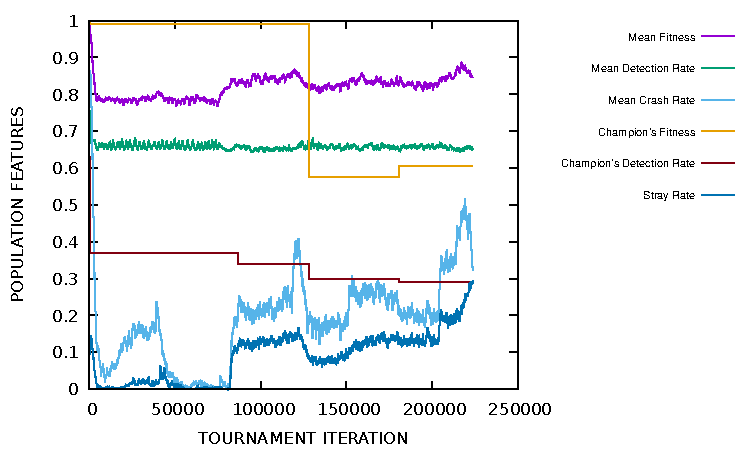
\includegraphics[width=.9\linewidth]{../images/plots/hepfap.pdf}
\caption{\label{fig:org4bc5928}
A run on the Iris classification task, with a high stray rate, by the \emph{Hepfap} population.}
\end{figure}

\begin{figure}[htbp]
\centering
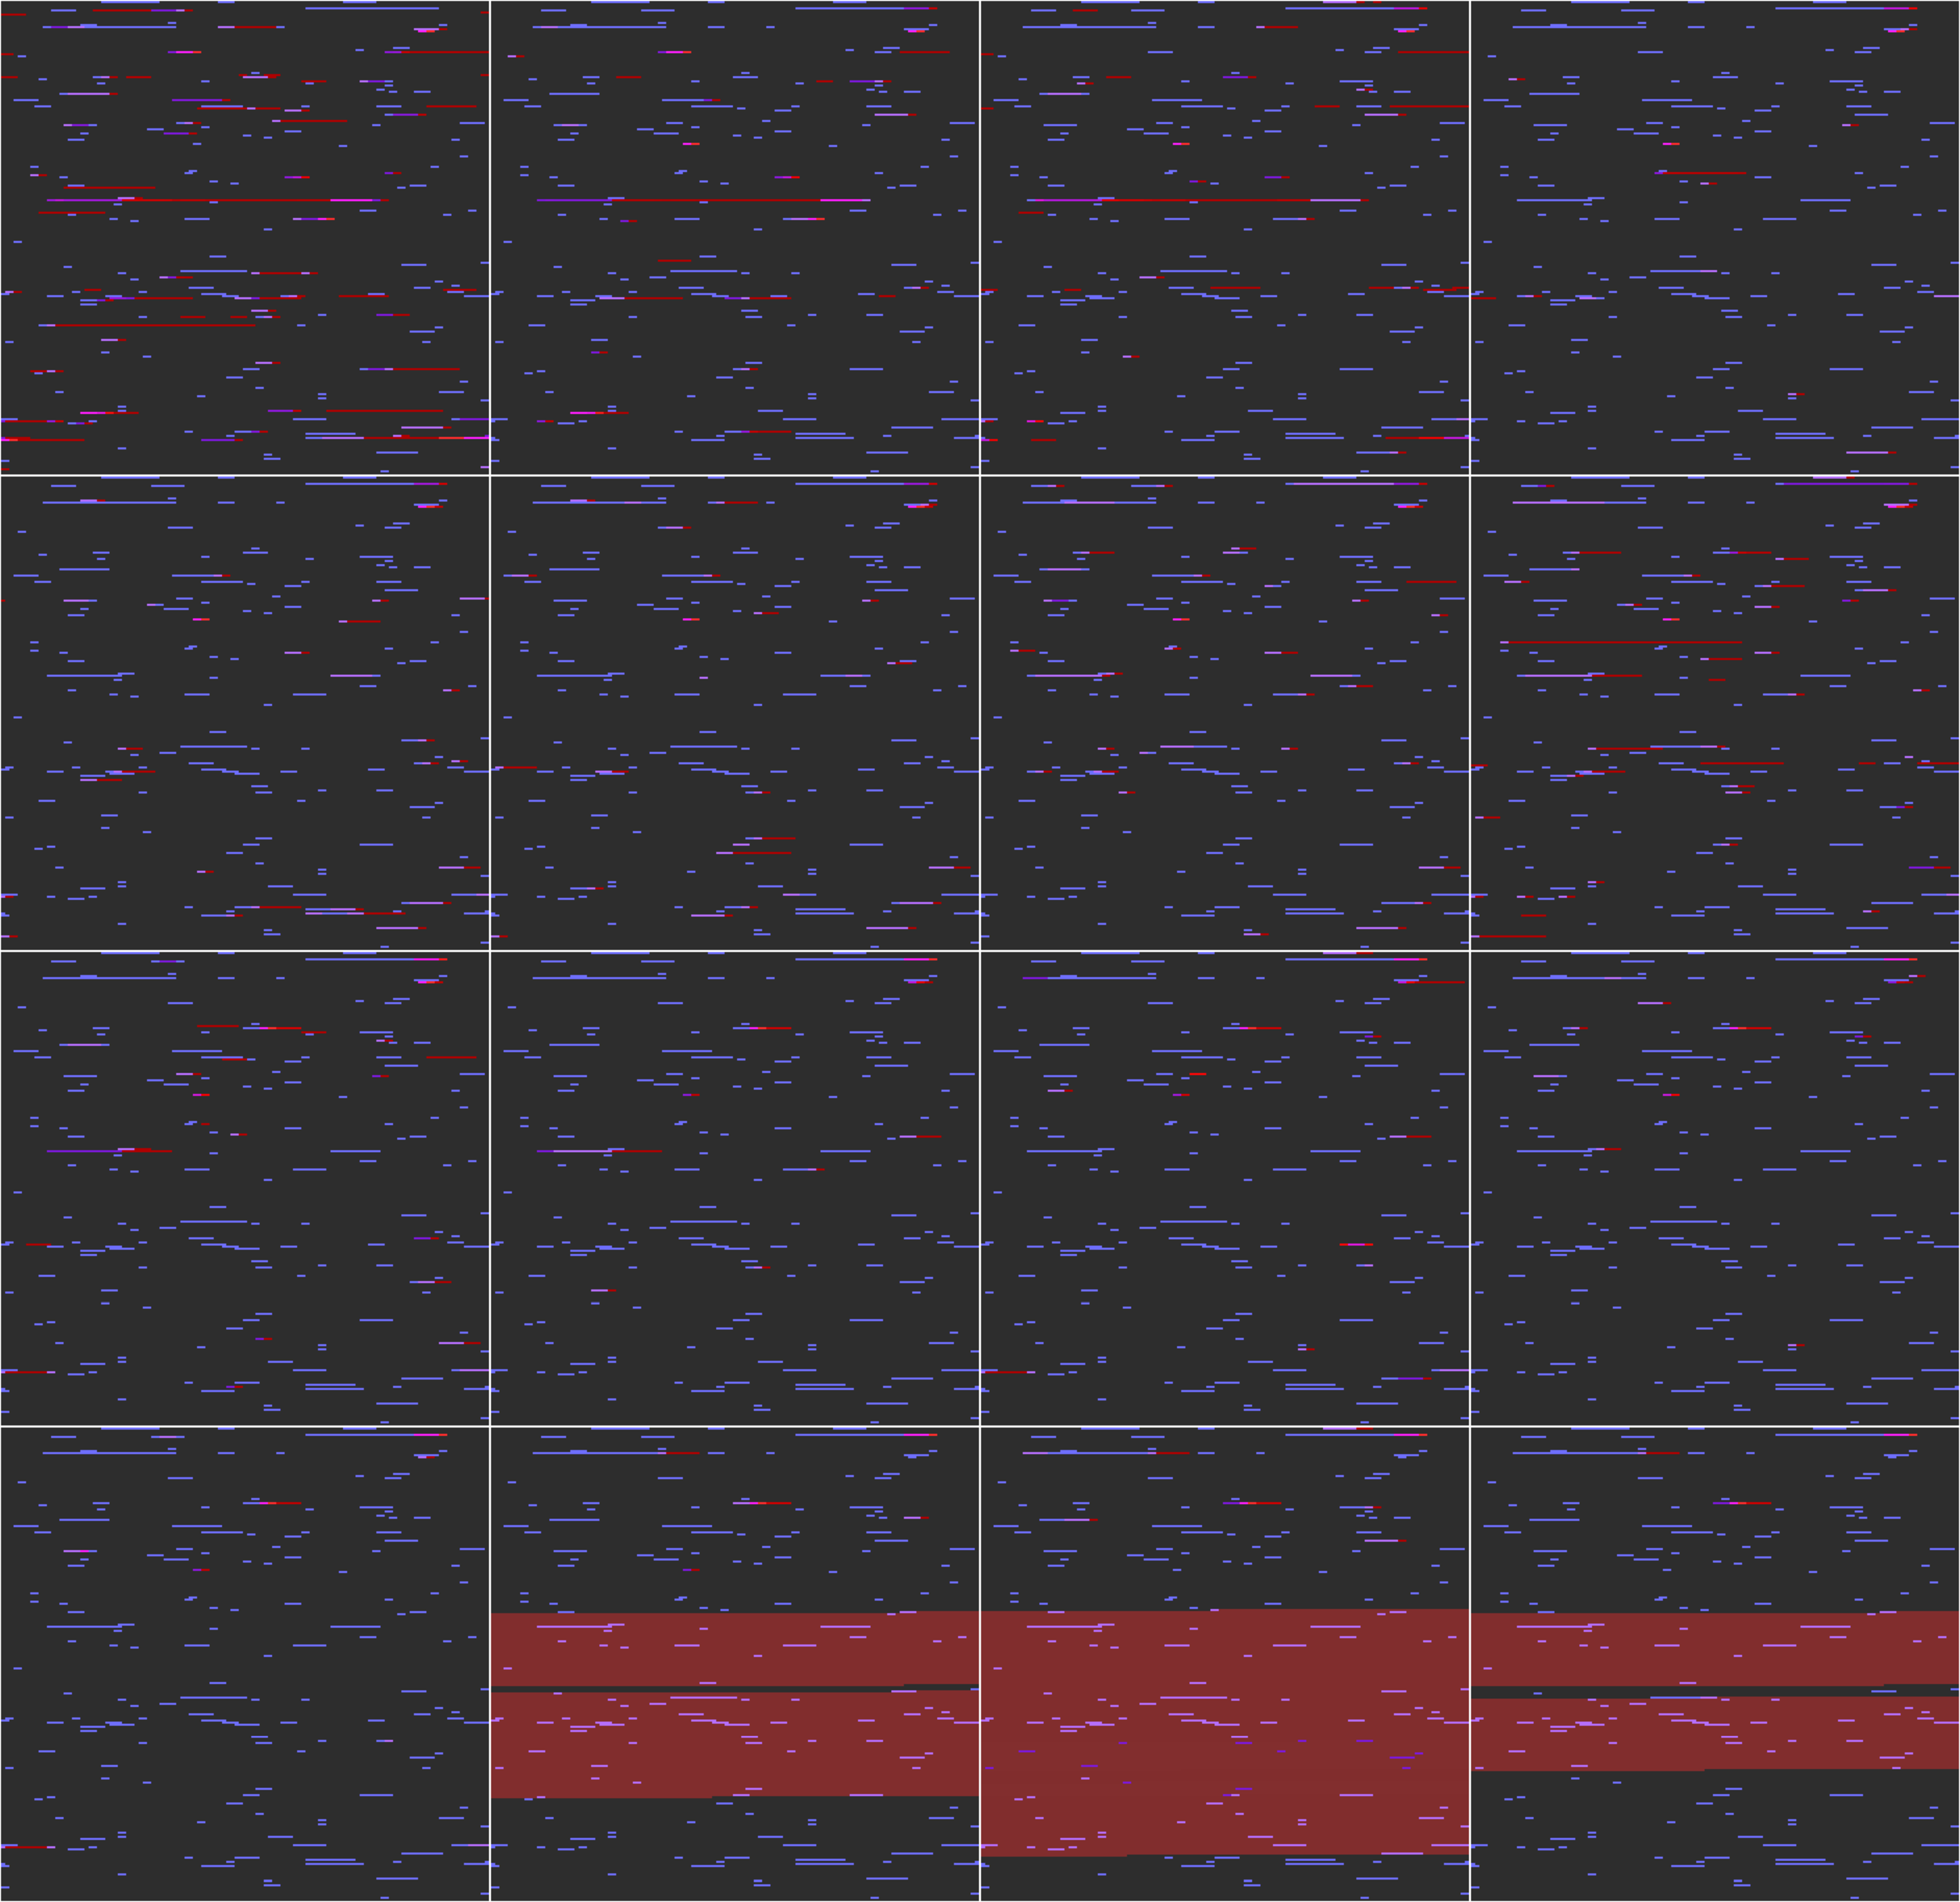
\includegraphics[width=.9\linewidth]{../images/plots/fimjek_heatmap_montage.pdf}
\caption{\label{fig:org7d6dce6}
Heatmap montage over the \emph{Fimjek} population, showing range of addresses executed, in red tint, superimposed on a map of the explicit gadgets that were harvested to form that population's initial gene pool, in blue tint. The intensity of red tint indicates the frequency with which the corresponding address was visited. Magenta and purple cells indicate orthodox gadget traffic, while red swaths with no tint of blue indicate stray activity. From top-left to bottom-right, each cell is a snapshot of the evolving heatmap at intervals of 20 seasons. The underlying gadget map is taken from the tomato-RT-N18U-httpd binary that we used in this experiment.}
\end{figure}

\subsection{A conjectural explanation of stray-rate fluctuations as a result of intron pressure}
\label{sec:org405a40e}
What pressures could possibly be driving the evolution of such strange
specimens? The canonical set of gadgets that the population inherits as its
primordial gene pool is noisy and brittle enough, but at least those gadgets are
selected for stability -- first, prior to each run, by our gadget harvesting
routines, which look for code fragments that are at least \emph{likely} to preserve
control flow, and then, throughout the run, by fitness pressures that penalize
the loss of execution control (chains which crash before completion, or which do
not reach the designated termination address within a fixed number of steps),
and genetic operators that will tendentially drop unreliable gadgets from the
gene pool. And yet we find a tendency for the population to occasionally favour
gadgets that overwrite the individual's own code stack, and branch to uncharted
regions of executable memory that have no direct representation in the set of
gadgets making up the gene pool.

This type of behaviour appears to proliferate at a certain phase of the
evolutionary trajectory, which is no doubt significant: it has a tendency to be
favoured by periods during which the average fitness of the population more or
less plateaus, and its standard deviation narrows.


As Bahnzaf and others have shown \cite{nordin95} \cite{banzhaf98}, these are typically the conditions
under which we should expect to see signs of an accelerating accumulation of
\emph{introns}, or non-coding genes, in the population. The reason for this, Bahnzaf
conjectures, is that as dramatic improvements in the performance of the
specimens, with respect to their explicit fitness function, become increasingly
difficult to attain, and as specimens more and more find themselves competing
against relative equals, the immediate selective pressures imposed by the
fitness function become less decisive in steering the course of the evolution.
The greatest differential threat to our specimens -- or, rather, to their
genetic lineages -- during such plateaus, is no longer the performance of their
immediate rivals, but the destructive potential of the genetic operators
themselves. There is very little, after all, to prevent crossover or even
mutation from mangling the genome beyond repair, and yielding dysfunctional
offspring. Unlike animals, plants, or any advanced life forms familiar to us
from nature, our creatures lack any sophisticated mechanism for ensuring the
homological transfer of genes in sexual reproduction. There is very little to
predispose crossover operations to preserve adaptive groupings of genes, or to
replace the genes of one parent with semantically similar genes from the other.
The only structural constraint that we have explicitly afforded to those
operations is a fairly lighthanded ``fragility'' mechanism, that, over time,
decreases the chance that crossover will break apart adjacent pairs of genes
that have historically (in terms of the individual's own genealogy) performed
well together. But this is a very mild constraint.

The gene lines best protected against such threats are those that are structured
in such a way that crossover is least likely to do damage, or to break apart
genes that are best kept together. A relatively simple way to achieve such
protection is to pad the genome with semantically meaningless, or ``non-coding'',
sequences. So long as the probability that any gene sequence will be affected by
the action of a genetic operator is inversely proportionate to the length of the
genome, increasing the genome's length by adding otherwise ineffectual sequences
makes it less likely for those operators to mangle it in a semantically
meaningful -- and \emph{a fortiori}, semantically maladaptive -- way.

Introns are therefore a valuable resource for the gene pool, and are favoured by
selection as soon as the threat posed by the genetic operators outweighs the
threat posed by immediate rivals. A particularly common form that introns may
take, and which we see in a variety of genetic programming systems, is a NOP
instruction, an instruction that does nothing, or some sequence of instructions
that semantically cancel one another out. In order to exploit that resource,
however, we need both a base language in which NOPs or NOP sequences are
relatively common, and latitude in the maximum length of the individuals, so
that introns can be freely padded onto the genome.

In the context of ROP chains, a NOP is just a gadget that returns without
performing any other operations. If we were dealing with gadgets defined over
the Intel instruction set, we could find these just by taking the address of
\texttt{RET} instructions. When it comes to \gls{arm}, however, such gadgets are
significantly rarer. We rarely find a pop instruction that \emph{only} pops into the
program counter, without tainting the other registers as well. For reasons of
efficiency, most compilers favour multipop instructions. Longer gadgets are even
less likely to execute without inducing side-effects. As we have already noted,
we simply do not have the luxury of a sleek, minimal, more or less orthogonal
instruction set, where each instruction performs a single, well-defined,
semantically atomic operation. Our instruction set will almost always be a noisy
assemblage of irregular odds and ends, in which the sort of introns we typically
encounter in genetic programming systems is rather uncommon.

Gadgets that overwrite or leap out of their own ROP stack, on the other hand,
are relatively easy to come by. Though they pose a tremendous risk to the gene
line, when it comes to first-order fitness, they offer access to an otherwise
scarce resource: they protect against damaging crossover operations, by
rendering the entire, unused sequence of gadgets that will be either overwritten
or avoided, an unbroken sequence of introns. Crossover and mutation can do
whatever they will to the lower regions of these aberrant genome without
inflicting any damage on adaptive clusters of genes.

It is uncertain that \gls{roper} would be able to discover these labyrinthine
passageways through its host if the selection pressure against errors
were more severe. The breaking of a fitness plateau, in most of the populations
observed, was forecasted by a momentary peak in the crash rate. This often
appears hand-in-hand with a periodic increase in genome length, which chimes
with some of Banzhaf's findings regarding the relation between intron bloat
and punctuated equilibrium in evolutionary processes \cite{banzhaf98}.
During such periods, length begins to increase as protective code bloat
and a preponderance of introns is selected for over dramatic improvements in
fitness, since it decreases the odds that valuable gene linkages will be
destroyed by crossover.\footnote{The analysis of code bloat and introns that we are drawing on here is
  largely indebted to the theory of introns from Chapter 7, and \S 7.7 in
  particular \cite{brameier07}}

We see this clearly enough in our champion ROP-chain displayed in
Table \ref{tab:labyrinthine}, where 29 of its 32 gadgets
do not contribute in any way to the chain's fitness -- though they do increase
the odds that its fitness-critical gene linkages will be passed on to its
offspring.

Branching to gadgets unlisted in the chain's own genome can be seen as a
dangerous and error-prone tactic to dramatically increase the proportion of
introns in the genome. Selection for such tactics would certainly explain the
tendency for the crash rate of the population to rise -- and to rise, typically,
a few generations before the population produces a new champion.

\subsection{Testing the Extended Gadgetry Conjecture with Explicitly Defined Introns}
\label{sec:org3bc416c}

The explanation given above for the strange behaviour observed seems to me to
be compelling enough on strictly theoretical grounds, but it still remains
to be seen if it can withstand experimental testing. If, as I have conjectured,
this behaviour appears because it represents a rich, even if risky, source of
introns, which our system has, in various ways, made a rare resource, then we
should expect to see it decrease in frequency as a consequence of introducing a
much safer supply of \textbf{explicit} introns into the gene pool.\footnote{The idea for the technique used here comes largely from Nordin, Francone, and
  Banzhaf's 1995 paper, ``Explicitly Defined Introns and Destructive Crosover in Genetic
  Programming'' \cite{nordin95}, but differs somewhat in implementation. Nordin et al. 
  incorporate into their intron units a mechanism similar to the ``fragility'' device
  I used in \gls{roper}: each has a weight associated with it that influences the likelihood of crossover occurring at that particular link. The \glspl{edi} used in 
\gls{roper} also have this feature, but only in virtue of the fact that each \gls{edi}
is also a normal clump. The ``fragility'' of a clump, in \gls{roper}, is adjusted over
the course of the run, in proportion to the running average its vehicles' fitness,
down genealogical lines, returning to the default fragility value when the link it precedes
is severed by the crossover operator, just like any other clump. 
The fragility of an \gls{edi} in \cite{nordin95}, by contrast, is
randomly perturbed on each inheritance event. In \cite{nordin95}, \glspl{edi} are formally distinct entities as compared to ``exons'', wheras in \gls{roper} \glspl{edi} are just \emph{explicitly disabled} codons
(clumps where \texttt{clump.enabled == false}), a property that is allowed to mutate through the course of the run. The dynamics observed in \gls{roper} as a consequence of introducing \glspl{edi}, however, are quite similar to those reported in \cite{nordin95}.} All we need to do is
to define a type of \texttt{clump} that doesn't code for any gadgets or immediates
in the actual payload, but which can still be manipulated by the genetic
operators. The simplest way to do this is just to attach an \texttt{enabled}
flag with each clump, which can be set to either \texttt{true} or \texttt{false}. When
\texttt{false}, the clump is ignored by the serialization procedure that prepares
the payload, so that it's never sent to the emulation engine. We will also
add a new mutation operator, which is able to toggle the \texttt{enabled} flag during
reproduction. This lets the intron serve the additional, potentially useful
purpose of acting as a repository for genetic information. If the selective
pressure responsible for ``extended'' or ``stray'' gadgets is indeed derivative
of the well-known pressure to generate introns, then these \glspl{edi} should 
be able to undercut their market share.

Patience, and an adaptively disadvantaged experimental setup, was eventually
rewarded with a compelling corroboration of the intron conjecture regarding
the proliferation of stray gadgets. 

Eight populations of \gls{rop} chains over the \texttt{tomato-RT-N18U-httpd} binary were
initialized with identical parameters, with the sole exception of the \gls{edi}
rate: four (\emph{xufmoc}, \emph{simtyn}, \emph{surjes}, and \emph{mycwil}) began with an \gls{edi}
rate of zero, with no further possibility of acquiring \glspl{edi} through
mutation. The other four (\emph{megkek}, \emph{huzqyp}, \emph{rofted}, and \emph{qatjaq}) were
initialized with an approximate 10\% \gls{edi} ratio, and a 5\% per-clump \gls{edi}
mutation rate -- meaning that in the event of a mutation, which occurs in 50\% of
reproduction events, the other 50\% being the result of single-point crossover,
each individual clump has a 5\% chance of being toggled. In the event of
crossover, the \texttt{enabled} flag is simply inherited, along with its clump,
unaltered. This is a fairly aggressive mutation rate, giving us a probability of
$$ \frac{\sum_{n-1} \frac{1}{20} * (1 - \frac{1}{20})^n}{2} $$ that at least one
clump in a chain of length \(n\) will be toggled on or off, in each reproduction
event.

The task component of the fitness function for these trials was to match a
precisely specified \gls{cpu} context, similar to the register-matching task
discussed in \S\S \ref{org86f0f05} and \ref{org753cc2a}, but
with one key difference, incorporating a recent update to the engine: the
population would be responsible for matching not just a series of immediate
register values, but correctly dereferencing pointers as well (but only up to
one degree of indirection). The exact
pattern in question, in \gls{roper}'s (updated) syntax, is:
\begin{verbatim}
0002cb3e,&0002cb3e,000000000,_,_,_,_,0000000b
\end{verbatim}
Corresponding to the preparation of the \gls{cpu} for the system call,
\texttt{execv("/bin/sh", ["/bin/sh"], NULL)}, with \texttt{/bin/sh} at address
\texttt{0x2cb3e}. We will be disregarding the fitness results for these experiments,
however. The populations were deprived of mutation operators, with the exception
of an \gls{edi} toggling mutation in the cases of \emph{xufmoc}, \emph{simtyn}, \emph{surjes}, and
/mycwil. Their task evaluation function was also hobbled, so that it would feed
them very little information regarding the proximity of the registers to a correct match -- nothing but the bitwise hamming distance, for both immediate and indirect register
values. They were designed to either fail indefinitely, or evolve for an extremely
long period of time before converging, the better to study their long-term
dynamics. 

The results, presented in figures \ref{fig:orgf252144} and
\ref{fig:org51b1882}, were found to corroborate the intron hypothesis,
though not as dramatically as anticipated. One of the four \gls{edi} populations
still showed a visible history of stray address visitation, but only one, as
compared to the four \gls{edi} free populations, all of which showed signs of
straying. Though fine-grained genealogical data is not available for these
populations, the relative continuity of the stray line in the \emph{Rofted} population, 
appearing in figure \ref{fig:orgf252144}, suggest that this \emph{may} be the
result of a single bloodline, in contrast to the \gls{edi} free \emph{surjes} and 
\emph{Simtyn} populations, where the incidence of strays appears in fits and starts, 
suggesting multiple genealogical origins. It would be interesting to repeat this
experiment with larger populations, and the collection of genealogical data, 
as time (and memory space for exponentially accumulating data) allow. 

The trajectory of the genome length curve in each population group is consistent
with what we know about introns and genetic bloat (cf. \cite{banzhaf98}), and
it is to be expected that the populations lacking \glspl{edi} would supplement
their absence with an accumulation of ``spare'' genes. But what's surprising is
that those same populations appear to be executing the majority of their
tremendously large genomes -- and doing so with relatively infrequent crashes. 
The non-\gls{edi} populations have an anomalous member in this respect, too:
the \emph{Xufmoc} population exhibits a sharp downwards trajectory in its genome
length, following its 2000\(^{\text{th}}\) season.  

A surprising result is the the non-\gls{edi} populations appear to have a higher
ratio of executed gadgets -- even though this ratio is calculated only with respect
to \emph{enabled} gadgets, excluding \glspl{edi}. The difference on this measure is rather
subtle, however, and may be the effect of noise, or overrepresented and idiosyncratic
bloodlines. 


\begin{figure}[htbp]
\centering
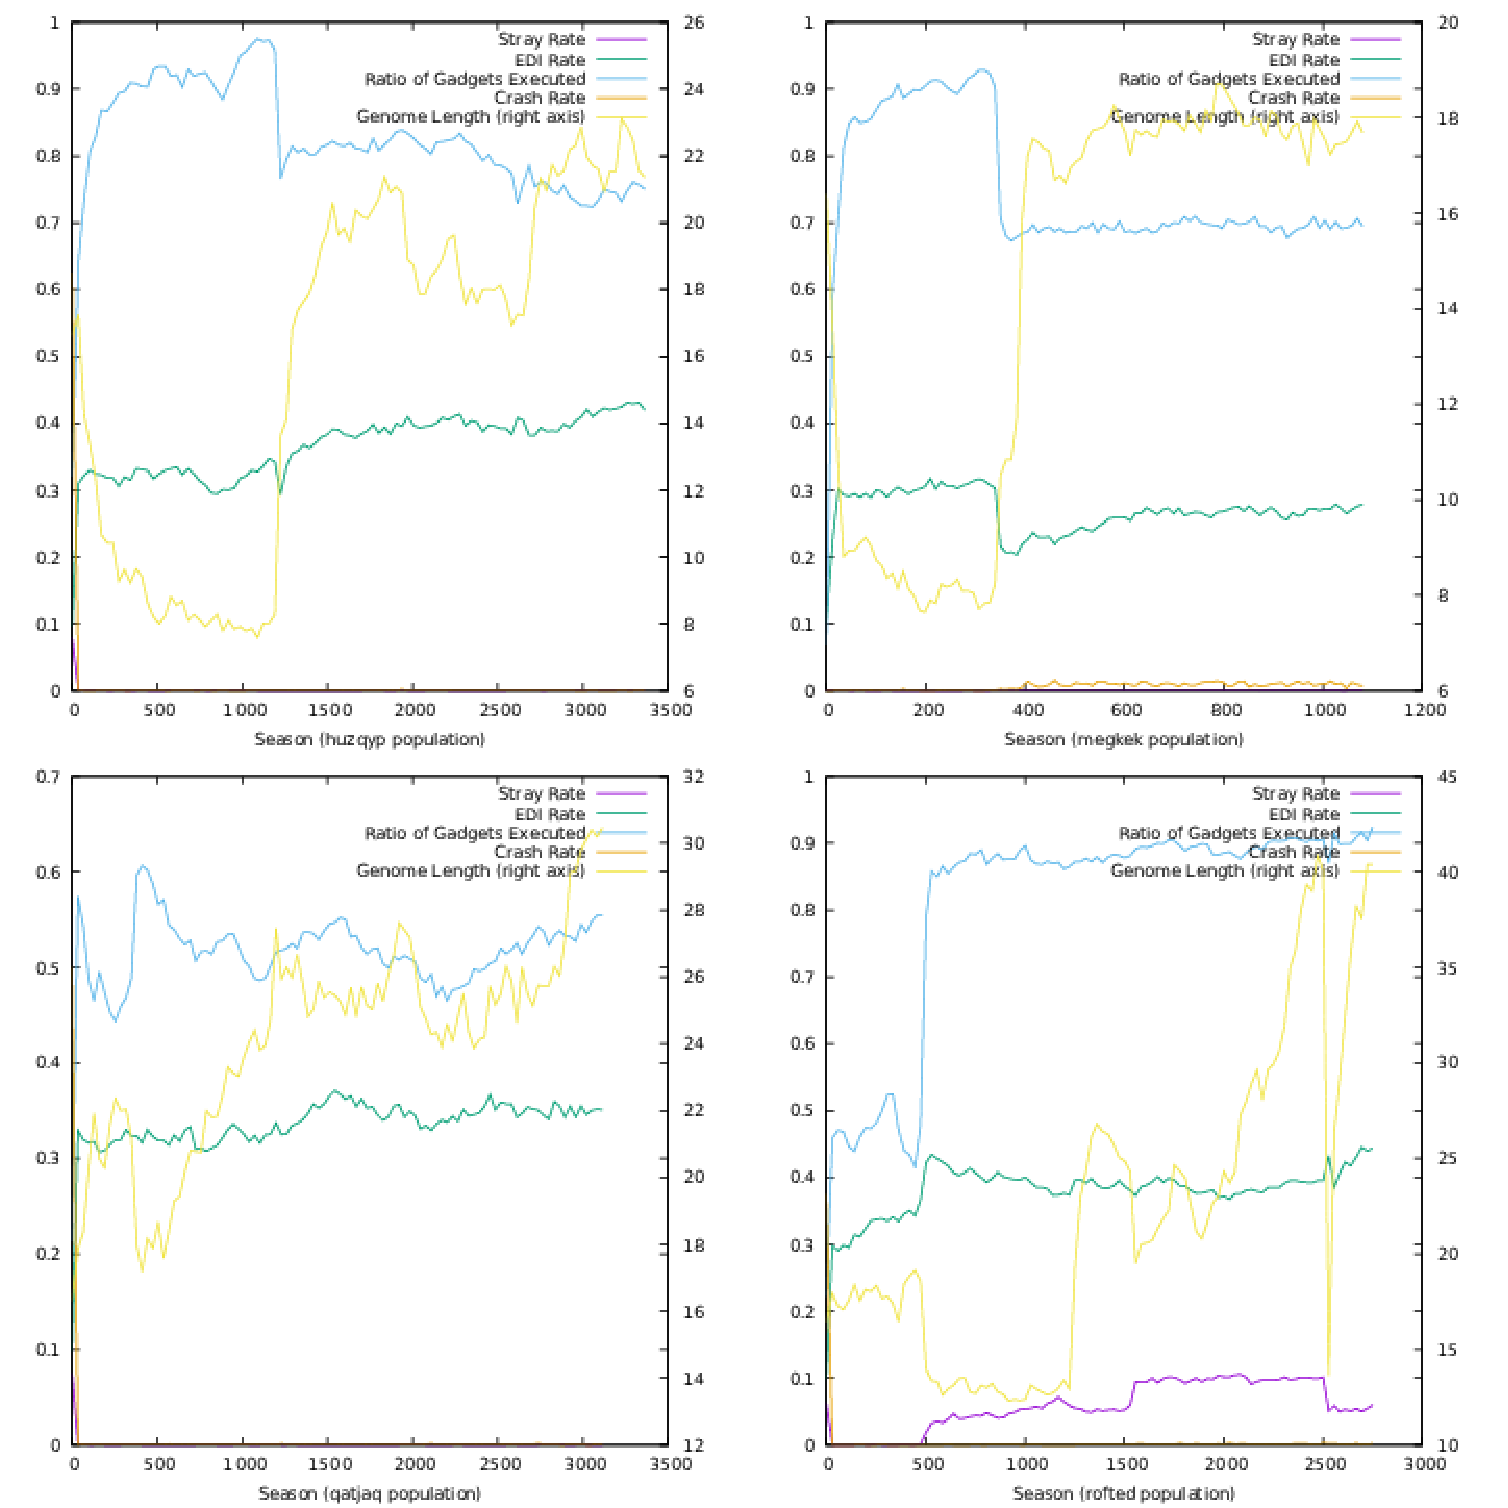
\includegraphics[width=.9\linewidth]{../images/plots/edi_stray_montage.pdf}
\caption{\label{fig:orgf252144}
Plot of EDI frequency to stray rate, crash rate, and the ratio of gadgets run in the \emph{hyzqyp}, \emph{megkek}, \emph{qatjaq} and \emph{Rofted} populations, with non-EDI mutation disabled.}
\end{figure}

\begin{figure}[htbp]
\centering
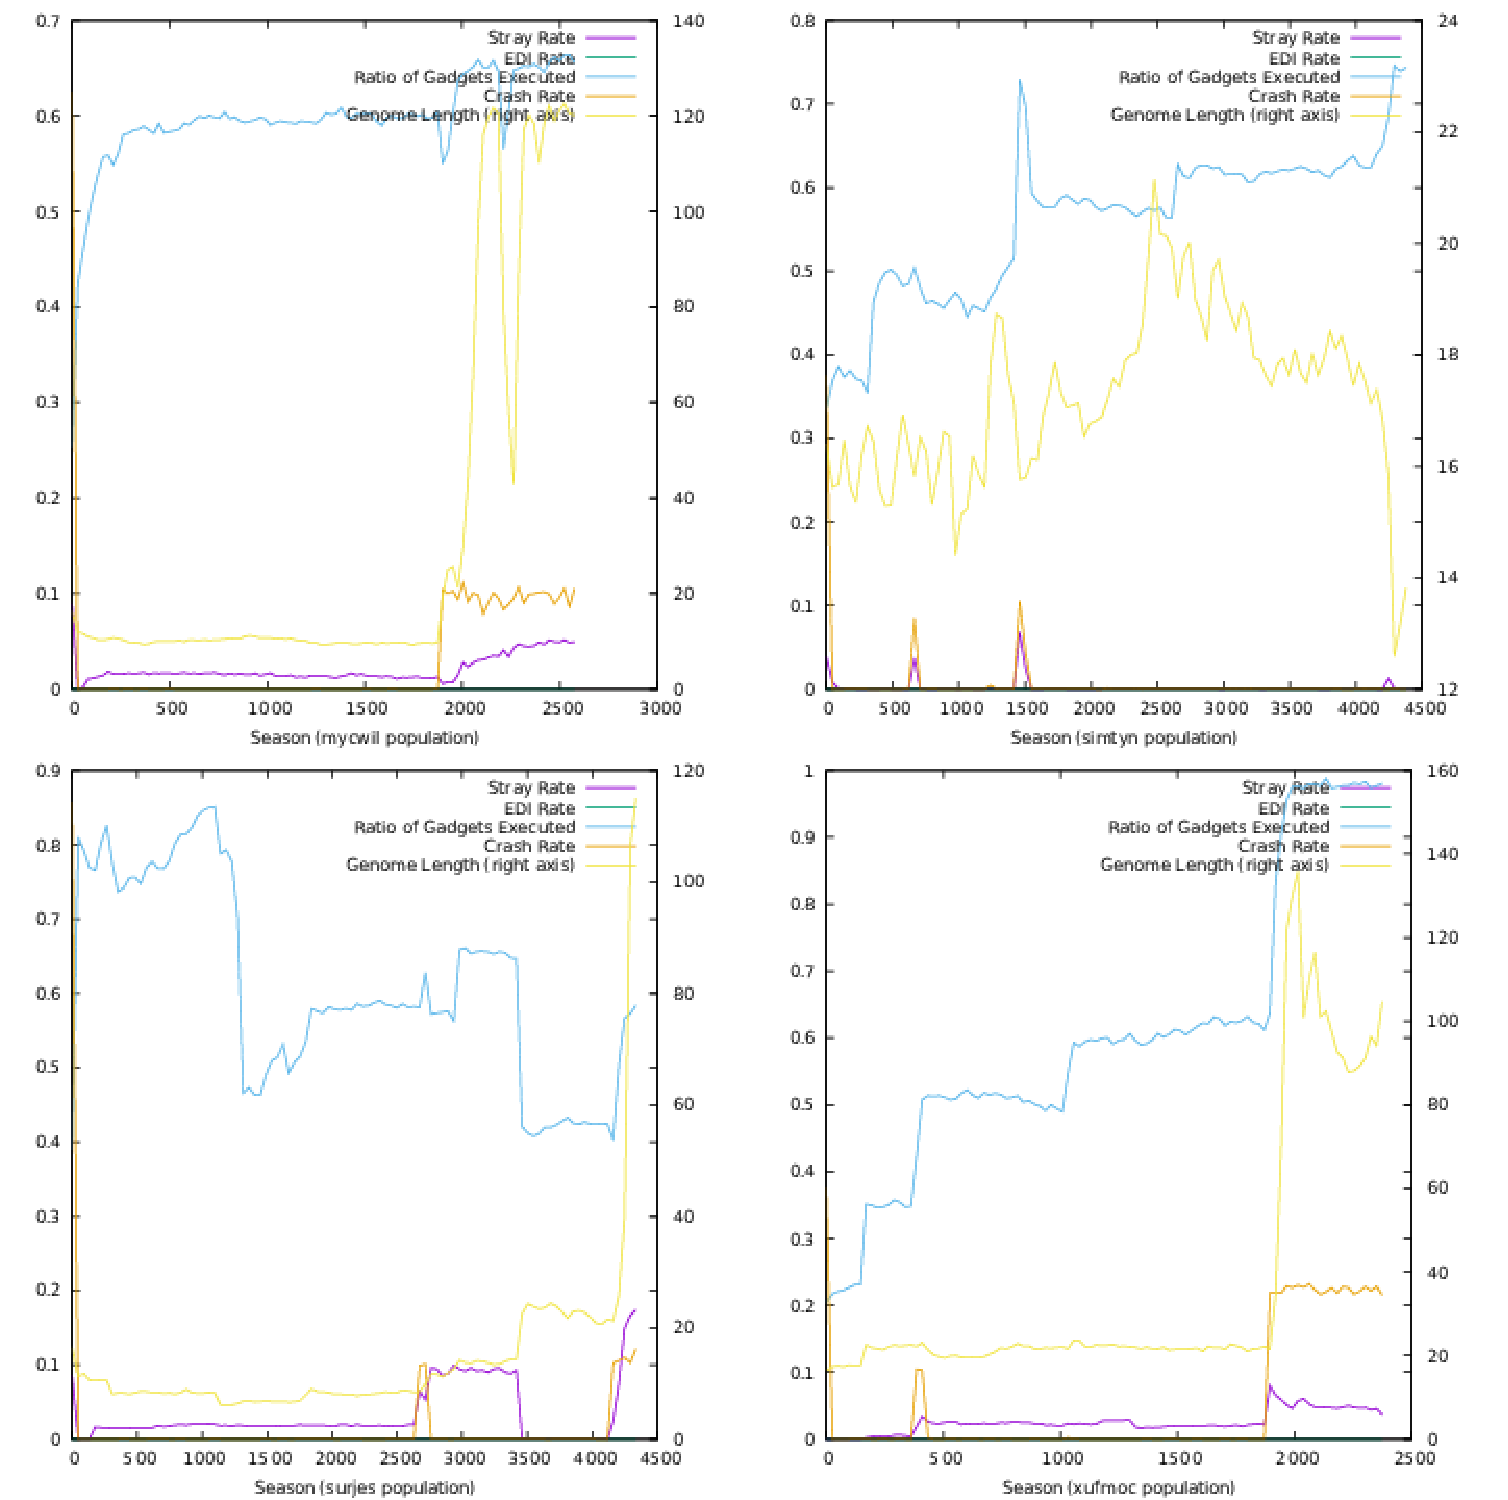
\includegraphics[width=.9\linewidth]{../images/plots/noedi_stray_montage.pdf}
\caption{\label{fig:org51b1882}
Plot of stray rate, crash rate, and the ratio of gadgets run in the \emph{mycwil}, \emph{simtyn}, \emph{surjes} and \emph{Xufmoc} populations, with mutation and EDI toggling disabled, with a base EDI rate of zero.}
\end{figure}

\chapter{Conclusions and Future Work}
\label{sec:org455cafe}
\label{orgca86428}

\section{The devil in the details}
\label{sec:orgcc88fc7}

\Gls{roper} has been explicitly designed as a ``proof of concept'', and not
as a refinement on existing prior art. The experiments documented here,
that is to say, represent the first glimpse we have had of the possibility
of \gls{rop} chain evolution. The application of an existing body of knowledge
and techniques -- here, genetic programming -- to an otherwise familiar
application domain, admittedly, seems to be something somewhat narrower than
a \emph{conceptual} innovation. 

But, on the one hand, the devil's in the details, and this is why I chose to
spend the majority of Chapter \ref{org8167c36} labouring over peculiarities
in individual cases and idiosyncracies in population trends, rather than focus
on accumulating quantitative performance metrics. What we find there, I think,
are challenges \emph{specific} to the domain of evolving populations of programs on
such ``weird machines'' as the \gls{rovm}. It is one thing to design a system that
is optimised and streamlined, from the ground up, for use in machine learning
or evolutionary computation, but it is something quite different to look for
ways to foster evolution in uneven assemblages of found materials. These are
assemblages that supervene on designed and documented machines, but which,
considered at the level of abstraction on which they operate, \emph{no one} has
designed, or documented, strictly speaking. No one \emph{builds} a \gls{rovm}; they
emerge accidentally through leaks in the procedural machine model around which
most software is designed and with an eye to which it is implemented. They
are systems that are \emph{discovered}, more than invented, even as they lie at
the heart of artificial and meticulously crafted systems. They form a sort
of junkyard wilderness at the heart of computational civilization. Their
exploration and study is the art of hackers, but this project began with the
intuition that something more might be learned of this strange terrain if
we approach it from the side of the wilderness, instead of from the side of
the explorer, and see how far we can get in coaxing unexpected structures 
and behaviours from it by applying just a bit of selective pressure, and
letting the system tell us about itself through the constraints it imposes 
on the resulting evolutionary process. 

And \gls{rop} is far from unique or special in this regard. The entire cybernetic
universe of processes and protocols is replete with accidental and supervenient
``weird machines'', unintentionally Turing-complete byproducts of their intentionally
designed substrates. From programmable \gls{elf} headers to javascript engine heap
allocators, the technological environment bristles with computational potential
that no one \emph{intended} to extend to its various, vulnerable interfaces. I believe
that the type of research conducted here, on the evolution of \gls{rop} chains, can
be fruitfully extended to these other strange domains, and many more.\footnote{For an ongoing compendium of ``weird machines'' and their exploitation by the
  hackers who love them, I direct the reader to the pages of \emph{PoC||GTFO}
  \cite{pocorgtfo}.} Very little
is necessary, after all, to create an evolutionary system, and with a bit of care
and craftsmanship, I believe that we can learn a great deal about what strange
forms of computation can be bred in the crevices of our familiar, algorithmic
abstractions. 

Exploring some of this terrain using the techniques employed above, and
extending them, is the first article of on my agenda of ``future work'',
after this project. Even within the framework of \gls{roper}, however, there
are a number of interesting open problems and refinements to be explored,
and I will use the remainder of this chapter to document a few of the most
pressing.


\section{Futher experiments and modifications suggested by above results}
\label{sec:org3d47335}

The reader will have noticed that Chapter \ref{org8167c36} raised at least
as many questions as it answered, and that only a fraction of them were dealt
with directly in that chapter. 

\subsection{Adding a \gls{ttl} field to clumps to contain malignancy and promote novelty}
\label{sec:orgd0524c7}

This was touched on in \S \ref{orgb6dff3e}, in response to an interesting case
of a malignant gene being aggressively promoted by selection, in virtue of the
beneficial trait with which its malignancy was indissociably bound. It's the
sort of problem to which evolution systems whose components are semantically
complex and multivalent are prone. Attempting to regulate it by tinkering with
the weight of a single, scalar fitness value involved tradeoffs whose merit was
difficult to anticipate in advance\footnote{It's possible that using a vectorial fitness value, and applying an algorithm
  like Pareto optimization, may be another way of sidestepping this problem, but
  that too remains to be explored in the context of \gls{roper}.}, and so another approach, orthogonal to the fitness mechanism, might be worth
exploring. It's implementation seems fairly straightforward, and it will be one
of the first experiments I perform with the system when time allows. 

\subsection{Collecting comprehensive genealogical data on the population during runtime}
\label{sec:orgaef0c83}

Frequently, in my analysis of various peculiar behaviours in \gls{roper}'s
populations, in Chapter \ref{org8167c36}, my enquiry was cut short by a simple
lack of data. It would be interesting to know, for example, \emph{just how often} a
fit chain descends from a crashing ancestor -- information that could be used in
calibrating an optimal crashing penalty or \gls{ttl}, for instance, and which would
be very interesting in its own right. There's nothing difficult in principle in
collecting such data, but doing so efficiently will be an interesting optimization
challenge. 

\subsection{Refactoring and optimization}
\label{sec:org7ec1c68}

I have a tendency to take new and ambitious projects as an opportunity to learn
a new language, and in the case of \gls{roper}, this was Rust. Unfortunately, this
means that the entire codebase is \emph{rife} with rookie cruft, and drowning in 
technical debt. The system needs a complete rewrite, and one made with polymorphism,
extensibility, and optimization in mind. This will let future experiments be 
performed faster, and future modifications easier to make, as new ideas present
themselves. The current state of the system has left the code difficult to reason
about, and cumbersome to modify. It is very much a first draft, and a beginner's
project. It was a joy to write, but I think it has long since outgrown its current
form, and very much deserves an overhaul -- one that includes unit tests and
documentation, to boot. 

\subsection{The Snake game, and other interactive problem spaces}
\label{sec:orgb183dd9}

The experiment touched on in \ref{org28ee8f8} remained largely tangential,
and it cries out for completion and more careful study. This, too, is on the agenda. 

\subsection{Testing ROPER's payloads on fully realized systems}
\label{sec:orgfb8251d}

In the experiments discussed above, we never went beyond studying the behaviour
of \gls{roper}'s populations \emph{in vitro}, trapped in their reasonably complete, but
still somewhat simplified and abstract emulated environment. It would be interesting
to see whether \gls{roper} can evolve specimens that can be used in a ``real world''
scenario -- testing them, at the very least, against a full-fledged \gls{qemu} instance
of a router, for example, with an actual \gls{rce} vulnerability as their point of
entry. This would mean \emph{much} slower evolutionary cycles, of course, but perhaps
a pipeline could be set up between the Unicorn ``nursery'' where the chains evolve 
until they reach a certain threshold of fitness, and a more fully realized \gls{vm}
where their \emph{in vivo} viability is put to the test. 


\section{Broader strokes}
\label{sec:org7de5ad3}

On the back burner, at present, sits a side project where I had begun to rewrite
\gls{roper} from scratch, before realizing that this was perhaps a bit too
ambitious, given the time constraints of the thesis. This overhaul was initiated
with an eye to what I took to be a handful of serious limitations in \gls{roper}'s
design (some of which are, at the same time, items of interest peculiar to \gls{roper}):


\begin{enumerate}
\item the programming interface that it exposes to the evolutionary
algorithm is brittle and uneven, and in no way optimized for evolvability;

\item the evolutionary process has little means of gaining traction
on the genotypes' program semantics -- in themselves, the genotypes are
little more than vectors of integers, and there is no way of acquiring any
information of how those vectors will behave, except for executing them --
and this is something at which each individual only ever gets a single
attempt;

\item the reproduction algorithms are fixed, and, as we have seen,
most frequently destructive. There is nothing inherent in crossover, or in
our mutation operations, that makes them well suited to the problem of
recombining ROP chains, or exploring the uneven, and largely uncharted,
semantic space that the execution of those chains represents. We may not
\emph{know} a better algorithm, but perhaps we could at least let \gls{roper}
explore other possibilities, itself, and expose the reproduction algorithms
themselves to evolutionary pressure.
\end{enumerate}

\subsection{``ROPUSH'' or ``ROPER II''}
\label{sec:org5fa6058}

A design idea for the second iteration of \gls{roper} was spurred by an
interesting suggestion made by Lee Spector, in a discussion of some of my
preliminary results and challenges at GECCO 2017 (where I presented \cite{fraser17_gecco}). Spector suggested that the
opacity and brittleness that I was grappling with in ``\gls{roper} I'' might become
more tractable if, instead of having the individuals of my population be more or
less direct representations of ROP-chain payloads, I instead evolved populations
of ROP-chain \emph{builders} -- programs that would compose ROP-chains from the
available materials, but which may, themselves, have a very different structure.

The ontogenetic map from genotype to phenotype would then consist of two phases,
rather than just one:

\begin{enumerate}
\item a mapping from the builder's code to a constructed payload, implemented
by executing the builder,

\item the mapping we're already familiar with, from \gls{roper}, which maps the
constructed payload (ROP chain) to the behaviour of the attack in the
emulated host.names
\end{enumerate}

The language in which the builders are defined could then be tailored to fit the
situation as well as possible -- pursuing a strategy similar to the one that
SPTH used in the design of Evolis and Evoris.

I decided to experiment with style of language that Spector had, himself,
introduced into genetic programming, and write a dialect of PUSH for this
purpose -- a statically typed, FORTH-like language that is designed with an eye
towards evolutionary methods rather than use by human programmers. Unhandled
exceptions, for instance, are effectively absent from the language, optimizing
it for mutational robustness rather than debugging and predictability.

At present, an initial implementation of a PUSH-style virtual machine, designed
for building \gls{rop} chains, that would then run on the Unicorn emulator -- for
which I wrote a basic library of Common Lisp bindings -- sits, like I said, on
the back burner of the current \gls{roper} git repository. It would be interesting
to see this through to completion, when time allows. 

\subsection{A return to Q, through the Binary Analysis Platform}
\label{sec:org2e769f6}

I've also become increasingly interested, lately, with the domain of semantic
binary analysis, and have been giving some though to switching from Unicorn
to \gls{bap} as my \gls{rop} chain evaluation framework. Here, I would be following
in the footsteps of \emph{Q} \cite{schwartz11}, one of the projects that had first
inspired me to work in this problem space. I'm interested in seeing where a 
marriage between \emph{Q}'s semantic-analysis driven compiler of programs for the
\gls{rovm}, and \gls{roper}'s evolutionary approach could take things. Having a
richer source of precise, semantic information to nudge the evolutionary process
through local hill-climbing searches, and a meaningful type system for gadgets
that could be used in fostering homologous crossovers and saner mutations, could
be an extraordinarily rich vein to mine. If \gls{roper} II ever sees the light of
day, it will probably try to move in this direction as well, using \gls{bap} to
extract type information and mediate evolutionary synthesis with intelligent
semantic analysis, with a highly flexible and evolvable, type-aware ROPUSH
abstraction layer coordinating those activities. 


Until then, I will tend to my \glspl{rop}.


\appendix
\chapter{Appendix: Recent Tweaks and Experiments}
\label{sec:org91594ee}
\section{Adjusting the classification task function for better environmental compatibility}
\label{sec:org7a3622d}
\subsection{Disadvantages of the bid-based algorithm in ROPER}
\label{sec:org5401e6a}
As we can see in figure \ref{fig:orgd9bb420}, the distribution of register use
in a fairly typical \gls{arm} \gls{elf} program is hardly even. This places a tremendous skew
on the relative likelihood of register use by an arbitrary individual in \gls{roper}'s
populations. And since the entire set of registers is initialized to the same, constant
set of values for each one, the ability of an individual to use the distribution of weights
in each register as a discriminant for a task is hamstrung from the outset. We are already
cutting the execution environment against the grain when we try to configure our
fitness functions in this way.
\subsection{Using R0 to decide}
\label{sec:orgb22d873}
\label{orgb366dd8}
The \gls{arm} \gls{abi} \cite{arm_abi} already gives us some useful hints here, which we can try to adhere to, to
make our fitness functions more harmonious with their environment. Like the x86, the \gls{arm}
\gls{abi} designates a particular register for the purposes of carrying a return value:
\begin{quote}
The manner in which a result is returned from a function is determined by the type of that
result [\ldots{}] A Fundamental Data Type that is smaller than 4 bytes is zero- or sign-extended
to a word and returned in r0.
\end{quote}
Though larger values can enlist other registers as vehicles -- ``a 128-bit containerized vector
is returned in r0-r3'', for example -- the sole use of r0 is by far the most common case, which
explains why we see it being given so great a preference in figure \ref{fig:orgd9bb420}. 

``Cutting with the grain,'' here, would mean adjusting our fitness function so that it hews a bit
closer to the expected behaviour of procedures in its host. We can try, in particular, to base
an individual's classification decisions (for the purposes of a classification task -- this doesn't
impact the syscall preparation task at all) on the contents of \texttt{R0}, alone. 

There are several ways we might do this: we could assign different integer ranges to each
class, and then choose the class whose range in which the value in \texttt{R0} falls. Deciding on 
a fair choice of ranges is a nontrivial problem, however, and will largely depend on the
vicissitudes of the binary under attack. 

We could allocate bit mask ranges to each class, and then the class for which \texttt{make\_mask(class) \& R0} 
has the most high bits. This remains close to the bid-based approach, but uses bit slices of a single
register to provide the ``ballot boxes'', rather than separate registers. As before, we could refuse
to assign points in the event of a tie: \texttt{0xffffffff} and \texttt{0x00000000}, for example,
should not designate any particular class, but be seen as a failure to choose -- which helps us
filter out quite a bit of noise and trivial decisions.  

Some experimentation showed, however, that slicing the 32-bit range into equal, contiguous
masks still results in a fairly significant skew in the early results, before selection has
gone to work: the lower 8 bits, for example, are consistently favoured, as are the top 8, since
they are set whenever the value in \texttt{R0} represents a negative integer. 

To balance the playing field, and ensure a bit of variety between runs, I used a simple algorithm
to allocate non-colliding, randomized masks to each class in the configuration stage of each run
(it's a crude, trial-and-error based, expensive algorithm, but negligibly so,
since it only needs to be performed once per run), such that the masks each contain an equal number
of ones, and have a boolean sum that has \(n\) ones, where \(n = 32 \mod |\text{classes}|\).

This method tends to give a more or less equal probability, it seems, to the base likelihood
of each class being chose, at least within one order of magnitude -- which is
sufficient, since we can let the fitness sharing mechanism sort out the
remaining disparities.

Results so far have been encouraging. A solution to the trivial classification problem, involving
two linearly separable blobs, was solved within minutes with a perfect detection rate, and a
more algorithmically interesting solution than we saw when using the register-bid approach
(which, I believe, encourages relatively trivial solutions that do not generalize well at all, in
the context of \gls{roper}, since the only way to properly weight the registers is often by simply
moving the attribute values back and forth between output registers, with minor tweaking --
resources for subtly manipulating values in the mid-range registers are just too scarce a resource
in \gls{roper}'s environment). See tables \ref{tab:xysxim-champ-red} and \ref{tab:xysxim-champ-blue},
for execution traces of the champion classifier, operating on exemplars of the red and blue classes,
respectively. What we see here is something we saw only rarely when using the register-bid algorithm,
and almost never in the champions produced by that algorithm -- even when we try to encourage it
by incorporating a per-case performance diversity metric into the fitness
function: a difference in control flow, where \gls{arm}'s own conditional
operators are used to decide on the course of action, given readings from a
particular exemplar. The decision point in these specimens is the \texttt{popeq}
instruction at address \texttt{0x0000cdd4}, which pops the stack if and only if the
\texttt{zero} flag had been set by the previous flag-setting instruction (here, \texttt{subs
 r4, r0, \#0}, at \texttt{0x0000cdd0}).

\begin{table}
\begin{lstlisting}
IN:  a3 fffffd6f
0000b4b4       | pop {r4, r5, r6, r7, r8, pc}
0000d9a8       | cmp r0, #0
0000d9ac       | moveq r0, r3
0000d9b0       | pop {r3, pc}
0001010c       | rsb r5, r5, r0
00010110       | cmp r5, #0x40
00010114       | movgt r0, #0
00010118       | movle r0, #1
0001011c       | pop {r4, r5, r6, pc}
0000cdd0       | subs r4, r0, #0
0000cdd4       | popeq {r4, r5, r6, pc}
0000cdd8 stray | ldr r1, [pc, #0x1c]
0000cddc stray | mov r2, r4
0000cde0 stray | mov r0, #0
0000cde4 stray | bl #0x59e0
000127c4 stray | push {r1, r2, r3}
000127c8 stray | push {r0, r1, r2, r4, r5, r6, r7, r8, lr}
000127cc stray | mov r6, r0
000127d0 stray | mov r5, #0x400
000127d4 stray | add r7, sp, #0x28
000127d8 stray | ldr r8, [sp, #0x24]
000127dc stray | mov r0, r5
000127e0 stray | bl #4294933396
0000a374 stray | add ip, pc, #0
0000a378 stray | add ip, ip, #0x1e000
0000a37c stray | ldr pc, [ip, #0x5a8]!
0000a138 stray | str lr, [sp, #-4]!
0000a13c stray | ldr lr, [pc, #4]
0000a140 stray | add lr, pc, lr
0000a144 stray | ldr pc, [lr, #8]!

R0 (bin): 00000000000000000000010000000000
\end{lstlisting}
\caption{Behaviour of the champion of the \emph{Xysxim} population, for a member of the red class. Input registers are \texttt{r2} and \texttt{r3}.}
\label{tab:xysxim-champ-red}
\end{table}

\begin{table}
\begin{lstlisting}
IN:  ffffff98 d
0000b4b4       | pop {r4, r5, r6, r7, r8, pc}
0000d9a8       | cmp r0, #0
0000d9ac       | moveq r0, r3
0000d9b0       | pop {r3, pc}
0001010c       | rsb r5, r5, r0
00010110       | cmp r5, #0x40
00010114       | movgt r0, #0
00010118       | movle r0, #1
0001011c       | pop {r4, r5, r6, pc}
0000cdd0       | subs r4, r0, #0
0000cdd4       | popeq {r4, r5, r6, pc}
0000d9ac       | moveq r0, r3
0000d9b0       | pop {r3, pc}
00016168       | add r0, r4, r0
0001616c       | pop {r3, r4, r5, pc}
0000ad94       | mov r0, r3
0000ad98       | pop {r4, pc}
0001228c       | add sp, sp, #0x364
00012290       | add sp, sp, #0x400
00012294       | pop {r4, r5, r6, r7, r8, sb, sl, fp, pc}

R0 (bin): 00000000000000000000000011101010
\end{lstlisting}
\caption{Behaviour of the champion of the \emph{Xysxim} population, for a member of the blue class. Input registers are \texttt{r2} and \texttt{r3}.}
\label{tab:xysxim-champ-blue}
\end{table}

\begin{figure}[htbp]
\centering
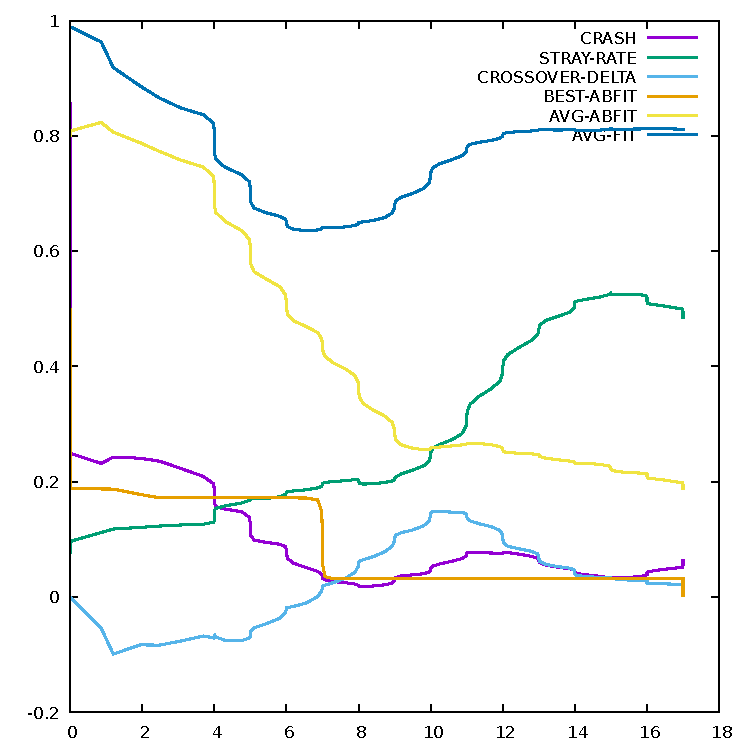
\includegraphics[width=.9\linewidth]{../images/plots/xysxim.pdf}
\caption{\label{fig:org8065e03}
Performance of the \emph{Xysxim} population on the simple, linearly separable dataset first encountered in \S \ref{orgbae8b45}.}
\end{figure}

This still leaves the matter of input registers, however. One mitigation of the uneven use of
input registers that has already been implemented in \gls{roper} is the possible use of the
stack to pass input parameters for each problem. This is done by associating with each
clump an \texttt{input\_slots} field, which tells the execution procedure to replace the values at
certain, specified stack indexes in the \gls{rop} payload with the available input values, which
offers much more flexibility, and adaptability, to the way the population handles input. 

\section{Homologous crossover}
\label{sec:org0d71cc5}
\label{org70e6edb}
\subsection{The trouble with crossover}
\label{sec:org3f0c1ad}
The trouble with crossover as it is currently implemented in \gls{roper}, and with
the way it is canonically specified in most standard forms of \gls{gp},
is that it is, as Nordin and others put it \cite{nordin99}, ``too \emph{brutal}'', and
insensitive to genomic context. The genome can be sliced more or less at random --
in \gls{roper}, tempered only slightly by the gentle weighting of splice-point probabilities
through the \emph{fragility} mechanism discussed in \ref{org7016026} -- combining and substituting
genes without any regard to their form or function.

\begin{figure}[htbp]
\centering
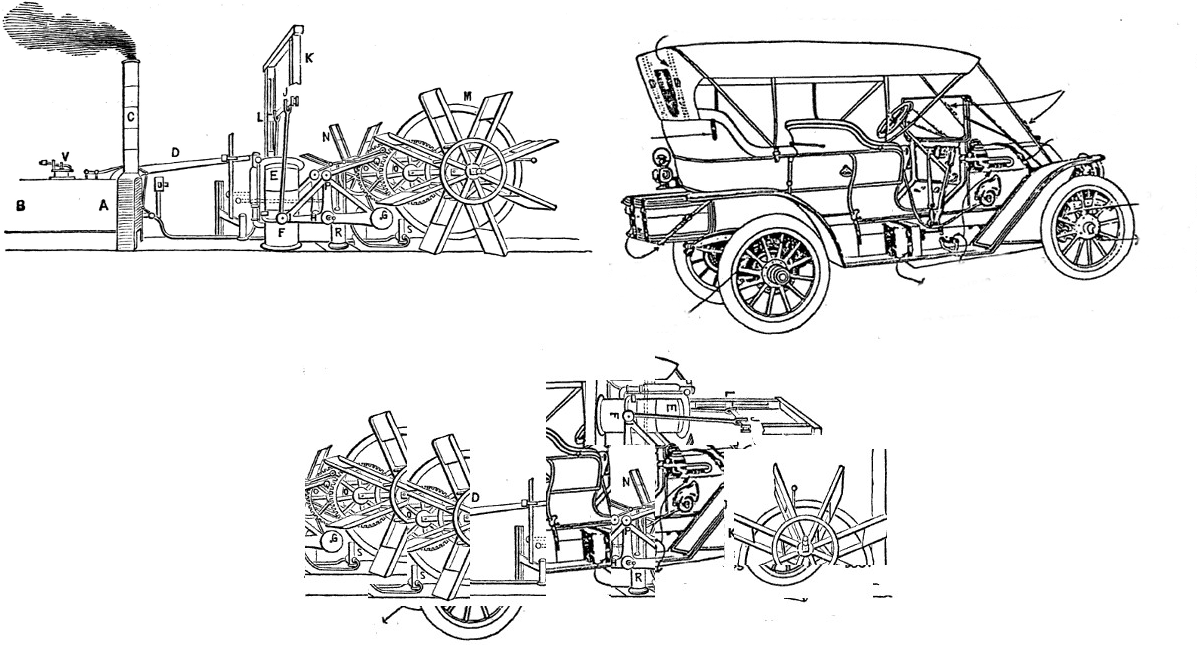
\includegraphics[width=.9\linewidth]{../images/carboat-montage.png}
\caption{\label{fig:org32569b8}
Unconstrained crossover in action}
\end{figure}

\subsection{One way of implementing (quasi-)homologous crossover in ROPER}
\label{sec:org4793a14}
In natural organisms, crossover is a highly constrained and sophisticated mechanism. 
Under ordinary circumstances, only those genes sharing the same loci in their respective
chromosomes are candidates for sexual recombination. This particular notion of ``loci'', 
however, has no genuine parallel in a canonical \gls{gp} system. It would be a mistake to
translate it, simply, as ``index'', since the ordering of a genome, at least at the beginning
of a run, has little structural significance with respect to function. A semantically richer
notion of structural position is desirable, here. Perhaps something like the \emph{return address}
of the gadget correlated with a clump can provide an indirect proxy for loci. This should at
least correlate, noisily, with phenotypic behaviour patterns, and can be
assessed in unit time (since it is already stored in the clump's metadata)
adding no further overhead to our crossover algorithm. 




Semantically meaningful organic structure tends to be extraordinarily scarce at the
beginning of a run, and there's no reason why we should trust a poorly
performing genome on having gotten anything ``right'' in the order of its genes.
We don't want to \emph{prematurely} constrain the possibilities of crossover, by enforcing
quasi-homological gene alignment on chains that may have very little interesting
organization in the first place. A sensible course of action would be to apply quasi-homological
constraints \emph{probabilistically}, where the probability of application is proportionate to
at least one parent's fitness. Algorithm \ref{alg:crossover-homo} shows one way
this could be done. 

\begin{algorithm}
\caption{Quasi-homologous Crossver, using Return Address Alignment}
\label{alg:crossover-homo}
\begin{algorithmic}[1]

\REQUIRE $(\vec{\mu}, \vec{\varphi})$: ([\![ \textbf{clump} ]\!], [\![\textbf{clump} ]\!]), the parental genotypes 
\REQUIRE \emph{fragility}: [\![\textbf{clump} ]\!] $\times$ [\![ \textbf{clump} ]\!] $\times$ lineage $\to \mathbb{F}$ 
\REQUIRE $(\mathfrak{R}, s)$: a PRNG and seed 
\REQUIRE $n$: $\mathbb{N}$, brood size


\STATE {$\mathfrak{R} \gets \textit{seed}(\mathfrak{R}, s)$} 

\STATE
{$t \gets \sum_{\mu \in \vec{\mu}} 1.0 - \text{fragilty}(\mu)$}

\STATE {$p, \mathfrak{R} \gets \text{random-float}(\mathfrak{R}, t)$} \COMMENT
{$p$ is more likely to fall on a highly fragile link} 
\STATE {$x \gets 0$}

\STATE {$\mu_i \gets 0$} 
\WHILE {$x < p$} 
  \STATE {$x \gets x + \text{fragility}(\mu_i)$} 
  \STATE {$\mu_i \gets \mu_i + 1$} 
\ENDWHILE 

\COMMENT {We now have the "mother's" splice point, $\mu_i$. With a probability proportionate to her fitness, look for a homolog in the "father".}
\STATE {$x, \mathfrak{R} \gets \text{random-float}(\mathfrak{R},1.0)$}
\IF {$x > \mu_{\text{fitness}}$ \AND $(n,\mu_{i_{\text{ret}}}) \in \{(c_{\text{index}}, c_\text{ret}) | c \in \phi\}$}

   \STATE {$\phi_i \gets n$}
\ELSE 
   \STATE {$\phi_i \gets $ a random index, using the algorithm above}
\ENDIF

\STATE {$\mu^a, \mu^b \gets $ split $\mu$ at $\mu_i$}
\STATE {$\phi^a, \phi^b \gets $ split $\phi$ at $\phi_i$}
\STATE {$\chi^a \gets \mu^a \cup \varphi^a$} \COMMENT {with metadata reinitialized and updated}
\STATE {\textbf{For $\chi^b$, repeat with sexes reversed}}
\RETURN {$\chi^a, \chi^b$} \COMMENT {the offspring}
\end{algorithmic} 
\end{algorithm}

The fecundity of this approach is the subject of ongoing experimental trials. 

\subsection{Alternative approaches to the problem}
\label{sec:org15d520e}

A more nuanced implementation of homologous crossover may be possible, using
runtime information gleaned from the execution of the parents -- we could
attempt to align clumps on the basis of a fuzzy match of their register states
at the moment of execution of their return instructions, perhaps. This would
capture the intuition of letting the paternal segment of the offspring \emph{pick up
where the maternal segment left off}, semantically speaking.


\section{Selecting for behavioural diversity}
\label{sec:org4ac972a}
\label{org204263f}

Fitness sharing, as currently implemented in \gls{roper}, skews the selective process
so as to favour diversity, on a problem-by-problem basis. I explain the algorithm
used in \S \ref{org48435b5}, and demonstrate its impact on classification tasks in 
Section \ref{orgf62a73d}. Its applicability, as we have seen, relies
on a discretely decomposable and repeating problem space, which is a serious limitation
when it comes to problem spaces where the variation is fine-grained or nonexistent:
neither the syscall preparation task (cf. \S \ref{org753cc2a}), which uses a
singleton problem set, nor the
Snake experiment (cf. \S \ref{org28ee8f8}), which uses a continuously
varying problem set, currently benefit from this approach. We might also wonder if
a more fine-grained favouring of diversity might be useful, even in problem spaces
where fitness sharing can be made to apply -- a metric that would reward diversity
even \emph{before} a problem is solved, and which would nudge the population towards
evolving a diversity of solutions to each problem, given that some approaches may
generalize better than others, in unforeseen ways. A more robust selection for
diversity in behaviour may also strengthen \gls{roper}'s potential to evolve 
obfuscated and ``heuristic-breaking'' payloads -- though, at this point, this remains
a speculative consideration, since we haven't yet built an apparatus that could
put this to the test. 

\Gls{roper} already has a wealth of generated data at is disposal, that could be
pressed into service, in this capacity: we are already tracking the execution
paths that each individual traces through the host process, for instance, but,
until now, we have only used this data for analytical purposes -- as seen,
throughout Chapter \ref{org8167c36}, in the analysis of heatmap data. 

I recently modified \gls{roper} so that the heatmap data collected can be threaded
through to the function responsible for fitness evaluation. This function now
scans the heatmap and normalizes the number of hits each address has received
into a float between 0.0 and 1.0 -- 1.0 indicating that the address is among
the most frequently visited, and 0.0 (or, rather, the absence of a value) 
indicating that it hasn't been visited at all. I then scan through the map of
addresses visited by a particular chain, on its most recent evaluation, and 
transform each into a weight by looking it up in the hashtable that represents
the normalized heatmap. These values are reduced to a mean, which indicates 
just how well-trodden that chain's path through the host is: a low value 
indicates that the chain took a path less travelled by, intersecting fewer
addresses visited before the
current tournament (or any running parallel to it), while a high value (closer
to 1.0) indicates that the chain took a more well-trodden path. This value
is then multiplied by a constant parameter \(v\) (which is tuneable, and currently
set to 0.2, on a whim), and summed with the existing fitness value times the
complement of \(v\): 
$$ \text{fitness} \gets (\text{novelty} * v) + (\text{fitness} * (1.0 - v))$$


\section{The clump TTL mechanism and the ecological role of extinction events}
\label{sec:org1397c3f}

Shortly after writing the conclusion to this thesis and submitting the examination
draft, I began experimenting with the \gls{ttl} mechanism on which I had pinned my
hopes for combating crash-prone but otherwise highly fit genes, which had shown a
tendency to spread malignantly through the population if left unchecked, under
the then-current configuration of \gls{roper}. 

During the initial chain spawning, each clump was assigned a \gls{ttl} field, set,
somewhat arbitrarily, to 16 (informed somewhat by observations on the generation
of well-performing chains, in various tasks -- but this was left tuneable). 

I adjusted the case evaluation algorithm, so that at the end of each chain's emulation,
it would store not only whether or not the chain had crashed, but the probable indices
of the clumps responsible for the crash, in one of its metadata fields. Those indices
were calculated on the basis of the return counter, which increments each time a return
address explicitly specified in the chain is visited. If the chain crashed with a
counter of \(n\), then it would be \emph{likely} (but not certain, due to straying) that
the \(n^{th}\) clump had at least a share in responsibility for the crash. 

In the crossover function, clumps with an index matching an entry in the crash log
would have their \gls{ttl} shifted one bit to the right. If this resulted in zero, the
clump would be dropped, and a new one generated on the spot, using the initial pool
of addresses for its first word, and constants recycled -- potentially repeatedly -- from
the dead clump. 

The result was far more disruptive to \gls{roper}'s ecologies than I had foreseen. 
Due to the relatively steadiness of the crash rate in most evolutions, over the
long term, the average \gls{ttl} values of each chain would tend to decline 
linearly, at first, until reaching a crisis point where numerous clumps would begin
to expire in unison. 
This is likely due, in part, to the irreversible heritability
of the \gls{ttl} field: it is passed intact by the crossover operator from parents to 
offspring, so that the crashes that decrement it need not be genealogically
contiguous. This would cause low \gls{ttl} counts to disseminate through the
population with surprising breadth, so that the final penalty of clump expiration
could be visited upon descendants quite distant from the highly crash-prone
ancestors responsible for diminishing the \gls{ttl}. 
This would lead, in turn, to mass extinction events in the population, as indexed in
the \emph{astronomically poor} turn taken by the crossover fitness delta metric in 
figure \ref{fig:org0c828d1} -- whose evolutionary run bore the same configuration as the population
in which the malignant gene problem was first diagnosed (see \S \ref{orgc22774b}).  

\begin{figure}[htbp]
\centering
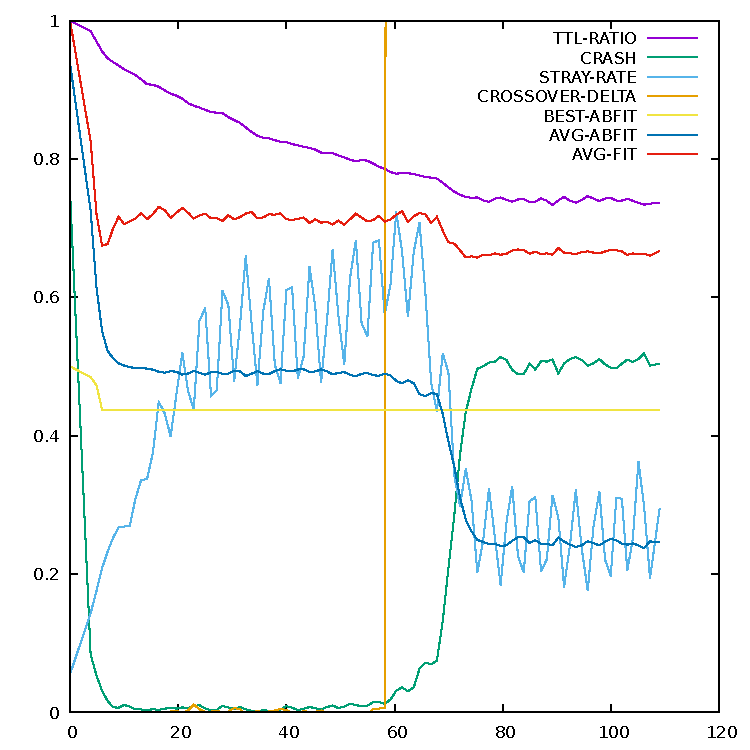
\includegraphics[width=.9\linewidth]{../images/plots/xilvyb.pdf}
\caption{\label{fig:org0c828d1}
Ecologically disruptive effects on the \emph{Xilvyb} population caused by the \gls{ttl} mechanism, causing a mass extinction of clump lines during a simple linear classification task, using register bid-bin classification.}
\end{figure}


The next experiment was conducted using the syscall preparation task. 
At the cost of an unusually slow convergence -- which may, perhaps, be
ameliorated by tuning some of our newly-introduced parameters -- the combination
of placing an expiration date on the last clump to execute in a crashing chain,
and introducing a selective incentive for behavioural diversity (see \S \ref{org204263f}) appears to yield
quite good results, so far as maintaining diversity is concerned. One such outcome
shows a distribution of address visitations that has no precedent in the populations
studied so far in this thesis: a run that terminated with \emph{greater} address visitation
diversity than it began with, while nevertheless, eventually, converging on a perfect
absolute fitness score. This occurred in the \emph{Soghuf} population, in the course of
completing the syscall preparation task, outlined in \S \ref{org86f0f05}.

The relatively low but nevertheless
steady rate of crashes in the population, which had settled into an equilibrium between
0.002 and 0.01 for most of the run, resulted in a sawtooth oscillation in the
mean \gls{ttl} rate, correlated, naturally, with massive, simultaneous clump die-offs at
repeating intervals. 

This had a strong impact on the fitness delta measurements for
the crossover operations, and a surprisingly large impact, it seems, on the stray
rate. To the extent that the \gls{ttl} mechanism serves an ecological function in
\gls{roper}, it appears to do so in a fashion comparable to forest fires, in the wild:
a periodic catastrophe, which keeps tendencies towards \emph{premature} convergence and
stagnation in check, but which nevertheless menaces even the fitter bloodlines in
the population with extinction. 

A modification could be made that lets a clump's \gls{ttl} be reset when
it appears in a non-crashing chain, or a non-crashing chain whose parents, too, were
free of crashes, and this may mitigate its ecological
impact somewhat. As currently implemented, the \gls{ttl} mechanic appears to be of
minor utility in problem spaces like those determined by the syscall preparation
task, but may be more useful when it comes to spaces in which premature
convergence is a problem that needs to be kept actively in check.



\begin{figure}[htbp]
\centering
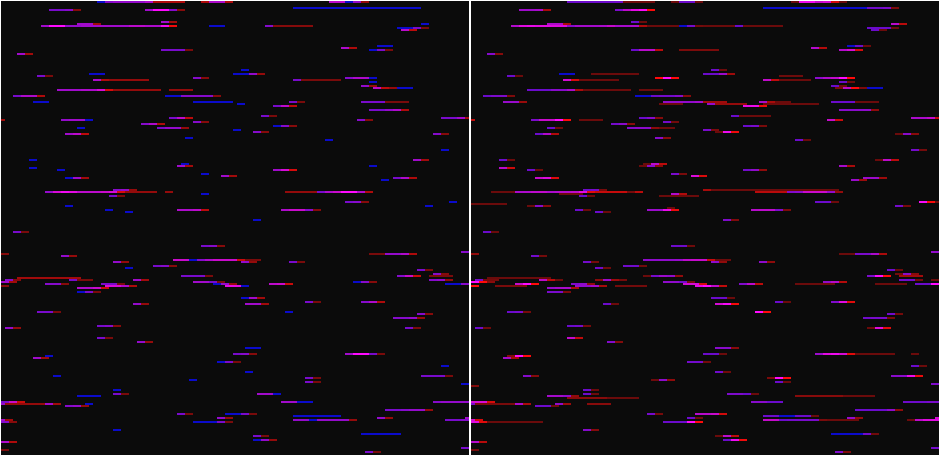
\includegraphics[width=.9\linewidth]{../images/plots/soghuf_heatmap_4_608.png}
\caption{\label{fig:orgb25a47d}
The effects of visitation novelty pressure on the \emph{Soghuf} population, with the additional influence of a \gls{ttl} field set to 4 and decremented on crash-prone clumps during crossover. The homologous crossover mechanism was not used for this run.}
\end{figure}

\begin{figure}[htbp]
\centering
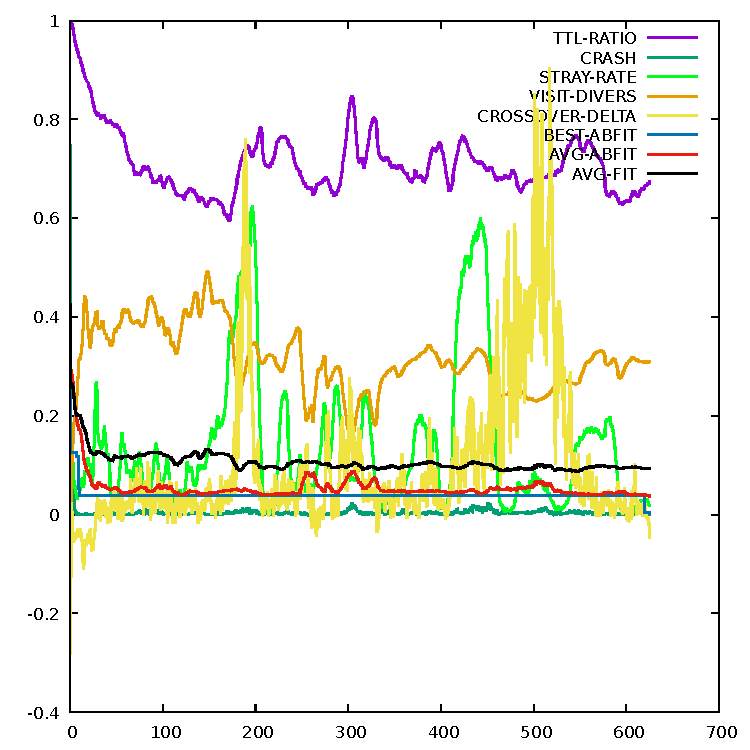
\includegraphics[width=.9\linewidth]{../images/plots/soghuf.pdf}
\caption{\label{fig:org57e618f}
Performance metrics over the \emph{Soghuf} population. Note mass extinction events around seasons 190, 300, and 400-500.}
\end{figure}



\section{Iris, Revisited}
\label{sec:orgff0e265}
Simple though it may be for systems engineered with no other task but classification in mind, the Iris dataset has 
proved to be a continual source of challenges for \gls{roper}. The superb run plotted in
\ref{fig:org2277148} was never equaled in subsequent trials. 

I recently revisited the dataset after implementing the modifications above, and, with
the exception of the \gls{ttl} mechanism, enabled them for a run on the Iris set. There
has not yet been time to complete a trial as lengthy as the one that gave us figure
\ref{fig:org2277148}, but the results so far have shown an extraordinary improvement over
their predecessors. The performance curves for this run are shown in figure \ref{fig:org2c028fc}. 



\begin{figure}[htbp]
\centering
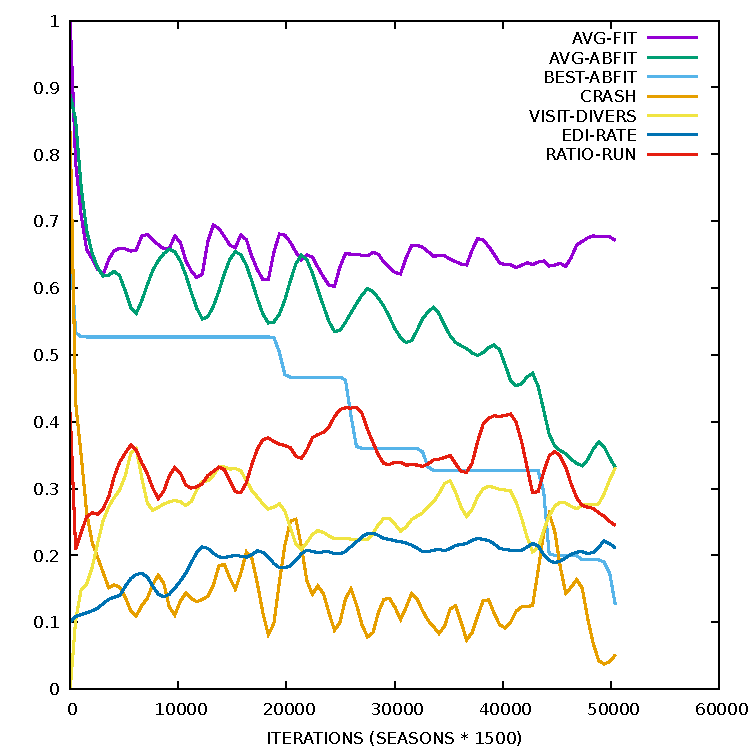
\includegraphics[width=.9\linewidth]{../images/plots/luxxyn.pdf}
\caption{\label{fig:org2c028fc}
Performance of the \emph{Luxxyn} population of 4096, over time.}
\end{figure}

\begin{figure}[htbp]
\centering
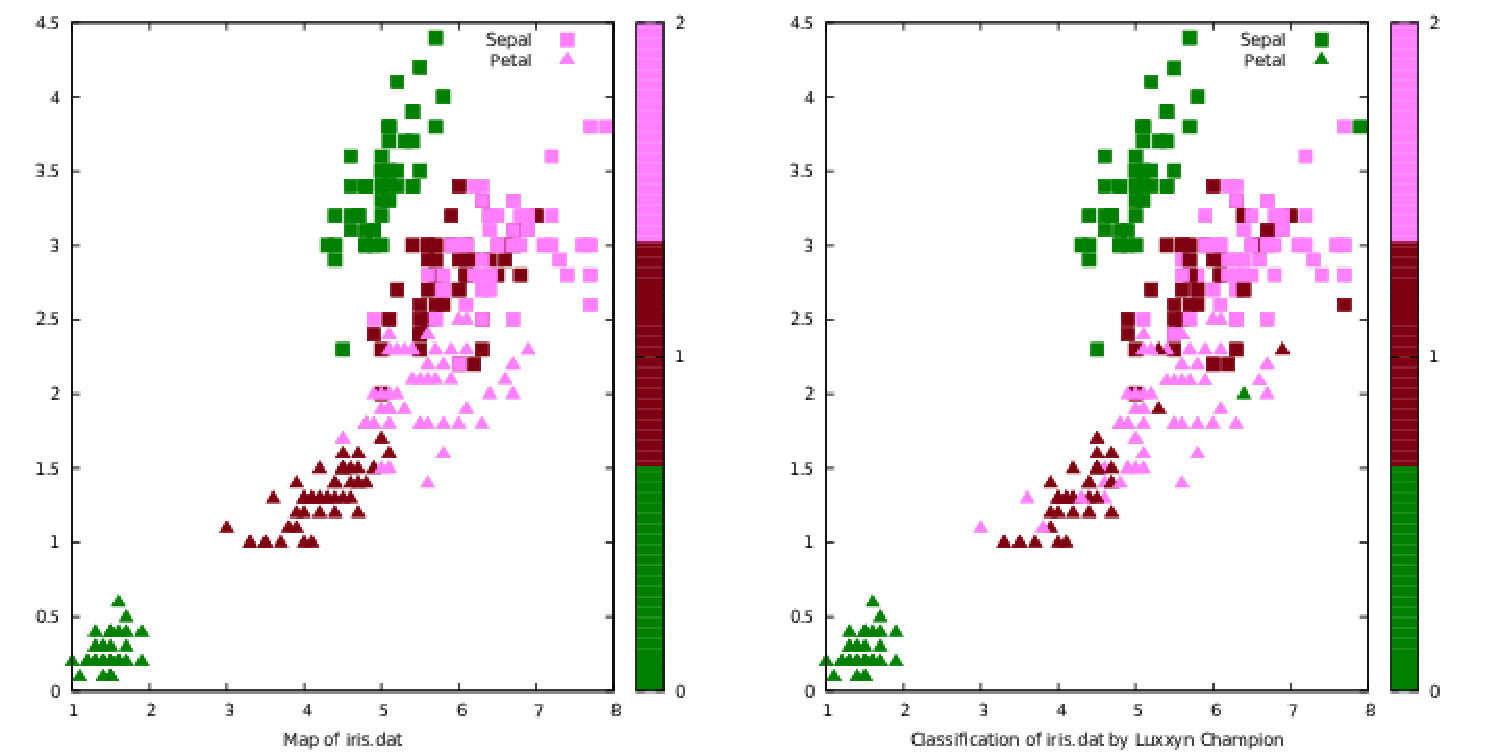
\includegraphics[width=.9\linewidth]{../images/plots/iris_with_luxxyn.pdf}
\caption{\label{fig:org6421f2a}
Comparison of the Iris dataset map with the classification performed by the \emph{Luxxyn} population's champion, after only 30 seasons.}
\end{figure}

As we can see in figure \ref{fig:org6421f2a}, \emph{even the linearly inseparable} 
regions of the Iris set were handled intelligently by the champion of this population
(the \emph{Luxxyn} population, the last we'll be considering in this thesis). 



\chapter{Appendix: Population Parameters}
\label{sec:org044f2ba}

\section{Note}
\label{sec:orgcde0005}
Here, the reader can find a series of tables documenting the critical parameters
used for each of the populations referred to by name in this thesis. The best source of
information on how, exactly, these parameters were implemented is the project's
(admittedly rather hairy) source code, at
\url{https://github.com/oblivia-simplex/roper}. The mutation rate, in each case,
is just the complement of ``crossover rate'', since each reproduction event
consisted in \emph{either} mating with crossover, or cloning with mutation. (This
does not hold for the 2017 populations, \emph{Poclux}, \emph{Cazmud} and \emph{Ragweb},
however. In those runs, crossover was used in every reproduction event, and
mutation was applied with the probability specified in ``mutation rate''. Numerous
differences in implementation also separate those experiments from the ones
conducted more recently. For details, please consult the git repository.)

The MD5 hash of the \texttt{tomato-RT-N18U-httpd} binary used in this series of
experiments is \texttt{16d38a233b45bab5b57476c11b066cfa}.

\section{Parameter Tables}
\label{sec:org1b346fd}
\begin{table}[htbp]
\caption{Parameters of the \emph{Cazmud} population, 2017/03/26.}
\centering
\begin{tabular}{lr}
binary & tomato-RT-N18U-httpd\\
brood size & 2\\
fitness goal & 0.1\\
fitness sharing & false\\
headless chicken rate & 0.15\\
input registers & [0, 1, 2, 3]\\
maximum length & 256\\
maximum start length & 32\\
migration & 0.05\\
minimum start length & 2\\
mutation rate & 0.9\\
number of demes & 4\\
output registers & [4, 5, 6]\\
population size & 2048\\
threads & 8\\
tournament size & 4\\
use fragility & false\\
use return counter & false\\
\end{tabular}
\end{table}

\begin{table}[htbp]
\caption{Parameters of the \emph{Fimjek} population, 2018/04/02.}
\centering
\begin{tabular}{lr}
binary & tomato-RT-N18U-httpd\\
brood size & 2\\
crossover rate & 0.2\\
edi toggle rate & 0\\
fitness goal & 0.1\\
fitness sharing & true\\
headless chicken rate & 0.15\\
initial edi rate & 0\\
input registers & [0, 1, 2, 3]\\
maximum length & 256\\
maximum start length & 32\\
migration & 0.05\\
minimum start length & 2\\
number of demes & 4\\
output registers & [4, 5, 6]\\
population size & 2048\\
threads & 4\\
tournament size & 4\\
use dynamic crash penalty & true\\
use fragility & false\\
\end{tabular}
\end{table}

\begin{table}[htbp]
\caption{Parameters of the \emph{Fizwej} population, 2018/04/09.}
\centering
\begin{tabular}{lr}
binary & tomato-RT-N18U-httpd\\
brood size & 2\\
crash penalty & 0.5\\
crossover rate & 0.5\\
edi toggle rate & 0\\
fitness goal & 0\\
fitness sharing & false\\
headless chicken rate & 0.15\\
initial edi rate & 0\\
input registers & [2, 3]\\
maximum length & 256\\
maximum start length & 32\\
migration & 0.05\\
minimum start length & 2\\
number of demes & 4\\
output registers & [0, 1]\\
population size & 2048\\
threads & 4\\
tournament size & 4\\
use dynamic crash penalty & false\\
use fragility & true\\
\end{tabular}
\end{table}

\begin{table}[htbp]
\caption{Parameters of the \emph{Hepfap} population, 2018/04/01.}
\centering
\begin{tabular}{lr}
binary & tomato-RT-N18U-httpd\\
brood size & 2\\
crossover rate & 0.2\\
edi toggle rate & 0\\
fitness goal & 0.1\\
fitness sharing & true\\
headless chicken rate & 0.15\\
initial edi rate & 0\\
input registers & [0, 1, 2, 3]\\
maximum length & 256\\
maximum start length & 32\\
migration & 0.05\\
minimum start length & 2\\
number of demes & 4\\
output registers & [4, 5, 6]\\
population size & 2048\\
threads & 4\\
tournament size & 4\\
use dynamic crash penalty & true\\
use fragility & false\\
\end{tabular}
\end{table}

\begin{table}[htbp]
\caption{Parameters of the \emph{Kathot} population, 2018/04/09.}
\centering
\begin{tabular}{lr}
population size & 2048\\
crossover rate & 0.5\\
tournament size & 4\\
brood size & 2\\
minimum start length & 2\\
maximum start length & 32\\
maximum length & 256\\
fitness goal & 0\\
headless chicken rate & 0.15\\
threads & 4\\
number of demes & 1\\
migration & 0.05\\
use fragility & true\\
output registers & [2, 3]\\
input registers & [0, 1]\\
binary & tomato-RT-N18U-httpd\\
fitness sharing & true\\
edi toggle rate & 0\\
initial edi rate & 0\\
crash penalty & 0.75\\
use dynamic crash penalty & false\\
\end{tabular}
\end{table}

\begin{table}[htbp]
\caption{Parameters of the \emph{Kurlig} population, 2018/04/10.}
\centering
\begin{tabular}{lr}
binary & tomato-RT-N18U-httpd\\
brood size & 2\\
crash penalty & 0\\
crossover rate & 0.5\\
edi toggle rate & 0\\
fitness goal & 0\\
fitness sharing & false\\
headless chicken rate & 0.15\\
initial edi rate & 0\\
maximum length & 256\\
maximum start length & 32\\
migration & 0.05\\
minimum start length & 2\\
number of demes & 4\\
population size & 2048\\
threads & 4\\
tournament size & 4\\
use dynamic crash penalty & false\\
use fragility & true\\
\end{tabular}
\end{table}

\begin{table}[htbp]
\caption{Parameters of the \emph{Luxxyn} population, 2018/04/16.}
\centering
\begin{tabular}{lr}
binary & tomato-RT-N18U-httpd\\
brood size & 2\\
class masks & 98694840:0 2282b112:1 0514062d:2\\
crash penalty & 0.5\\
crossover rate & 0.5\\
edi toggle rate & 0.3\\
fitness goal & 0.15\\
fitness sharing & true\\
headless chicken rate & 0.15\\
homologous crossover & true\\
initial edi rate & 0.1\\
input registers & [3, 4, 5, 6]\\
maximum length & 256\\
maximum start length & 32\\
migration & 0.05\\
minimum start length & 2\\
number of demes & 4\\
output registers & [0]\\
population size & 2048\\
threads & 6\\
tournament size & 4\\
ttl & 64000\\
\end{tabular}
\end{table}


\begin{table}[htbp]
\caption{Parameters of the \emph{Misjax} population, 2017/04/20.}
\centering
\begin{tabular}{lr}
binary path & tomato-RT-N18U-httpd\\
crossover rate & 0.3\\
population size & 4096\\
threads & 1\\
tournament size & 5\\
number of demes & 4\\
migration & 0.05\\
game seeds & randomized and unique\\
game board radius & 9\\
initial snake length & 5\\
number of apples & 2\\
number of cacti & 2\\
\end{tabular}
\end{table}


\begin{table}[htbp]
\caption{Parameters of the \emph{Poclux} population, 2017/03/22.}
\centering
\begin{tabular}{lr}
binary path & tomato-RT-N18U-httpd\\
brood size & 2\\
fitness goal & 0\\
headless chicken rate & 0.15\\
maximum length & 256\\
maximum start length & 32\\
migration & 0.1\\
minimum start length & 2\\
mutation rate & 0.45\\
number of demes & 4\\
population size & 1024\\
threads & 8\\
tournament size & 4\\
use fragility & true\\
\end{tabular}
\end{table}

\begin{table}[htbp]
\caption{Parameters of the \emph{Ragweb} population, 2017/03/26.}
\centering
\begin{tabular}{lr}
binary & tomato-RT-N18U-httpd\\
brood size & 2\\
fatal crash & false\\
fitness goal & 0.1\\
fitness sharing & true\\
headless chicken rate & 0.15\\
input registers & [0, 1, 2, 3]\\
maximum length & 256\\
maximum start length & 32\\
migration & 0.05\\
minimum start length & 2\\
mutation rate & 0.45\\
number of demes & 1\\
output registers & [4, 5, 6]\\
population size & 2048\\
threads & 4\\
tournament size & 4\\
use fragility & true\\
use return counter & false\\
\end{tabular}
\end{table}



\begin{table}[htbp]
\caption{Parameters of the \emph{Rofted} population, 2018/04/04.}
\centering
\begin{tabular}{lr}
binary & tomato-RT-N18U-httpd\\
brood size & 2\\
crossover rate & 0.2\\
edi toggle rate & 0.05\\
fitness goal & 0\\
fitness sharing & false\\
headless chicken rate & 0.15\\
initial edi rate & 0.1\\
input registers & [1, 2, 3, 4]\\
maximum length & 256\\
maximum start length & 32\\
migration & 0.05\\
minimum start length & 2\\
number of demes & 4\\
population size & 2048\\
threads & 4\\
tournament size & 4\\
use fragility & true\\
\end{tabular}
\end{table}

\begin{table}[htbp]
\caption{Parameters of the \emph{Simtyn} population, 2018/04/04.}
\centering
\begin{tabular}{lr}
binary & tomato-RT-N18U-httpd\\
brood size & 2\\
crossover rate & 0.2\\
edi toggle rate & 0\\
fitness goal & 0\\
fitness sharing & false\\
headless chicken rate & 0.15\\
initial edi rate & 0\\
input registers & [1, 2, 3, 4]\\
maximum length & 256\\
maximum start length & 32\\
migration & 0.05\\
minimum start length & 2\\
number of demes & 4\\
population size & 2048\\
threads & 4\\
tournament size & 4\\
use dynamic crash penalty & true\\
use fragility & true\\
\end{tabular}
\end{table}

\begin{table}[htbp]
\caption{Parameters of the \emph{Soghuf} population, 2018/04/05.}
\centering
\begin{tabular}{lr}
binary & tomato-RT-N18U-httpd\\
brood size & 2\\
crash penalty & 0.2\\
crossover rate & 0.5\\
headless chicken rate & 0.15\\
edi toggle rate & 0.3\\
fitness goal & 0\\
fitness sharing & true\\
homologous crossover & false\\
initial edi rate & 0.1\\
input registers & [1, 2, 3, 4]\\
maximum length & 256\\
maximum start length & 32\\
migration & 0.05\\
minimum start length & 2\\
number of demes & 4\\
population size & 2048\\
tournament size & 4\\
ttl & 16\\
threads & 4\\
use dynamic crash penalty & true\\
use fragility & true\\
\end{tabular}
\end{table}

\begin{table}[htbp]
\caption{Parameters of the \emph{Wiwzuh} population, 2018/04/07.}
\centering
\begin{tabular}{lr}
binary & tomato-RT-N18U-httpd\\
brood size & 2\\
crossover rate & 0.2\\
edi toggle rate & 0\\
fitness goal & 0\\
fitness sharing & false\\
headless chicken rate & 0.15\\
initial edi rate & 0\\
input registers & [1, 2, 3, 4]\\
maximum length & 256\\
maximum start length & 32\\
migration & 0.05\\
minimum start length & 2\\
number of demes & 4\\
population size & 2048\\
threads & 4\\
tournament size & 4\\
use fragility & true\\
use dynamic crash penalty & true\\
\end{tabular}
\end{table}

\begin{table}[htbp]
\caption{Parameters of the \emph{Xeqcyv} population, 2018/04/10.}
\centering
\begin{tabular}{lr}
binary & tomato-RT-N18U-httpd\\
brood size & 2\\
crash penalty & 0.2\\
crossover rate & 0.5\\
edi toggle rate & 0\\
fitness goal & 0\\
fitness sharing & true\\
headless chicken rate & 0.15\\
initial edi rate & 0\\
maximum length & 256\\
maximum start length & 32\\
migration & 0.05\\
minimum start length & 2\\
number of demes & 4\\
population size & 2048\\
threads & 1\\
tournament size & 4\\
use dynamic crash penalty & false\\
use fragility & true\\
\end{tabular}
\end{table}

\begin{table}[htbp]
\caption{Parameters of the \emph{Xilvyb} population, 2018/04/16.}
\centering
\begin{tabular}{lr}
binary & tomato-RT-N18U-httpd\\
brood size & 2\\
crash penalty & 1\\
crossover rate & 0.5\\
headless chicken rate & 0.15\\
edi toggle rate & 0.3\\
fitness goal & 0\\
fitness sharing & true\\
homologous crossover & false\\
initial edi rate & 0.1\\
input registers & [2, 3]\\
maximum length & 256\\
maximum start length & 32\\
migration & 0.05\\
minimum start length & 2\\
number of demes & 4\\
output registers & [0, 1]\\
population size & 2048\\
tournament size & 4\\
ttl & 16\\
threads & 4\\
use dynamic crash penalty & true\\
use fragility & true\\
\end{tabular}
\end{table}

\begin{table}[htbp]
\caption{Parameters of the \emph{Xufmoc} population, 2018/04/03.}
\centering
\begin{tabular}{lr}
binary & tomato-RT-N18U-httpd\\
brood size & 2\\
crossover rate & 0.2\\
edi toggle rate & 0\\
fitness goal & 0\\
fitness sharing & false\\
headless chicken rate & 0.15\\
initial edi rate & 0\\
input registers & [1, 2, 3, 4]\\
maximum length & 256\\
maximum start length & 32\\
migration & 0.05\\
minimum start length & 2\\
number of demes & 4\\
population size & 2048\\
threads & 4\\
tournament size & 4\\
use dynamic crash penalty & true\\
use fragility & true\\
\end{tabular}
\end{table}

\begin{table}[htbp]
\caption{Parameters of the \emph{Xysxim} population, 2018/04/13.}
\centering
\begin{tabular}{lr}
binary & tomato-RT-N18U-httpd\\
brood size & 2\\
class masks & (random; data lost)\\
crash penalty & 1\\
crossover rate & 0.5\\
edi toggle rate & 0\\
fitness goal & 0\\
fitness sharing & true\\
headless chicken rate & 0.15\\
initial edi rate & 0\\
input registers & [2, 3]\\
maximum length & 256\\
maximum start length & 32\\
migration & 0.05\\
minimum start length & 2\\
number of demes & 4\\
output registers & [0]\\
population size & 2048\\
threads & 4\\
tournament size & 4\\
use dynamic crash penalty & false\\
use fragility & true\\
\end{tabular}
\end{table}



\bibliographystyle{ieeetr}
\bibliography{thesis}
\end{document}